\chapter{Математичне моделювання та статистичний експеримент}
\label{chap:testing}

\section{Пошук у синтетичному сигналі}
    В цьому підрозділі розглянемо пошук шаблону в сигналі, що був згенерований як певна композиція неперервних
    функцій.

    Для початку порівняємо методи пошуку шаблонів використовуючи сигнал із шаблоном, котрий був доданий без
    будь"=яких видозмінень (окрім адитивного шуму/трансформації).

    В рамках експерименту на проміжку ${[0; 10]}$ із частотою дискретизації 10~КГц будувався сигнал, що складався
    з 8--16 гаусіан нормального розподілу $\dfrac{1}{\sigma\sqrt{2\pi}}
    e^{\frac{{\left(x-\mu\right)}^2}{2\sigma^2}}$
    (кількість гаусіан і їх параметри обиралися випадковим чином).
    До цього сигналу (бази) у випадкову позицію додавався шаблон виду $\sin{\alpha x^2}$.
    Приклад такого сигналу наведений на рисунку~\ref{fig:signal}.

    Результати статистичного експерименту наведено в таблиці~\ref{tab:simple-signal-results} на
    сторінці~\pageref{tab:simple-signal-results}.

    На рисунку~\ref{fig:simple-signal} на сторінці~\pageref{fig:simple-signal} наведені відповідні ефектограми
    нормалізованої взаємокореляції, нормалізованої суми квадратів відстаней та методу на основі поліномів Кунченко.
    Як видно з цих ефектограм, всі розглянуті методи досить точно знаходять шаблон у штучному сигналі.
    Але, як видно з таблиці результатів, середній час роботи методу поліномів Кунченка значно більший за час роботи
    існуючих методів.

    На рисунку~\ref{fig:simple-signal-kun-p} на сторінці~\pageref{fig:simple-signal-kun-p} наведені проміжні
    ефектограми поліномів Кунченка при застосуванні пірамідального пошуку для прискорення роботи алгоритму з трьома
    проміжними шарами: 100, 1000 та 10\,000 Гц відповідно.

    На прикладі, що зображений на цьому рисунку видно, що на першому шарі було знайдено 4 екстремуми, що були більшими
    за поріг 0,3.
    Околи отриманих екстремумів були розглянуті на наступному шарі, де було знайдено лише один екстремум, більший за
    поріг 0,01
    На наступному кроці в околі цього екстремум було уточнене значення ефектограми.

    Таким чином, результати статистичного експерименту показали, що якщо використовувати штучні сигнали для оцінки, то
    метод поліномів Кунченка має приблизно таку ж саму точність пошуку, що й розглянуті існуючі методи, а використання
    пірамідального пошуку дозволяє отримувати той самий результат навіть швидше за них.

    \stepcounter{tablecount}
    \begin{table}
        {|p{0.2\textwidth}|p{0.2\textwidth}|p{0.27\textwidth}|p{0.15\textwidth}|}
        {Результати пошуку шаблону без модифікації}
        {tab:simple-signal-results}
        {\hline
            & Час, с & Абсолютна похибка & Екстремум\\
            \hline}
        Kunchenko & 120,01 & -0,02 & 0,05\\
        NCC       & 5,95   & -0,02 & 0,24\\
        NSSD      & 5,78   & -0,02 & 1.52\\
        Kunchenko + Пирамідальний пошук & 0,81 & -0,02 & 0,05\\
    \end{table}

    \stepcounter{figurecount}
    \begin{figure}[h]
        \centering
        \subfloat[Без шуму]{%
            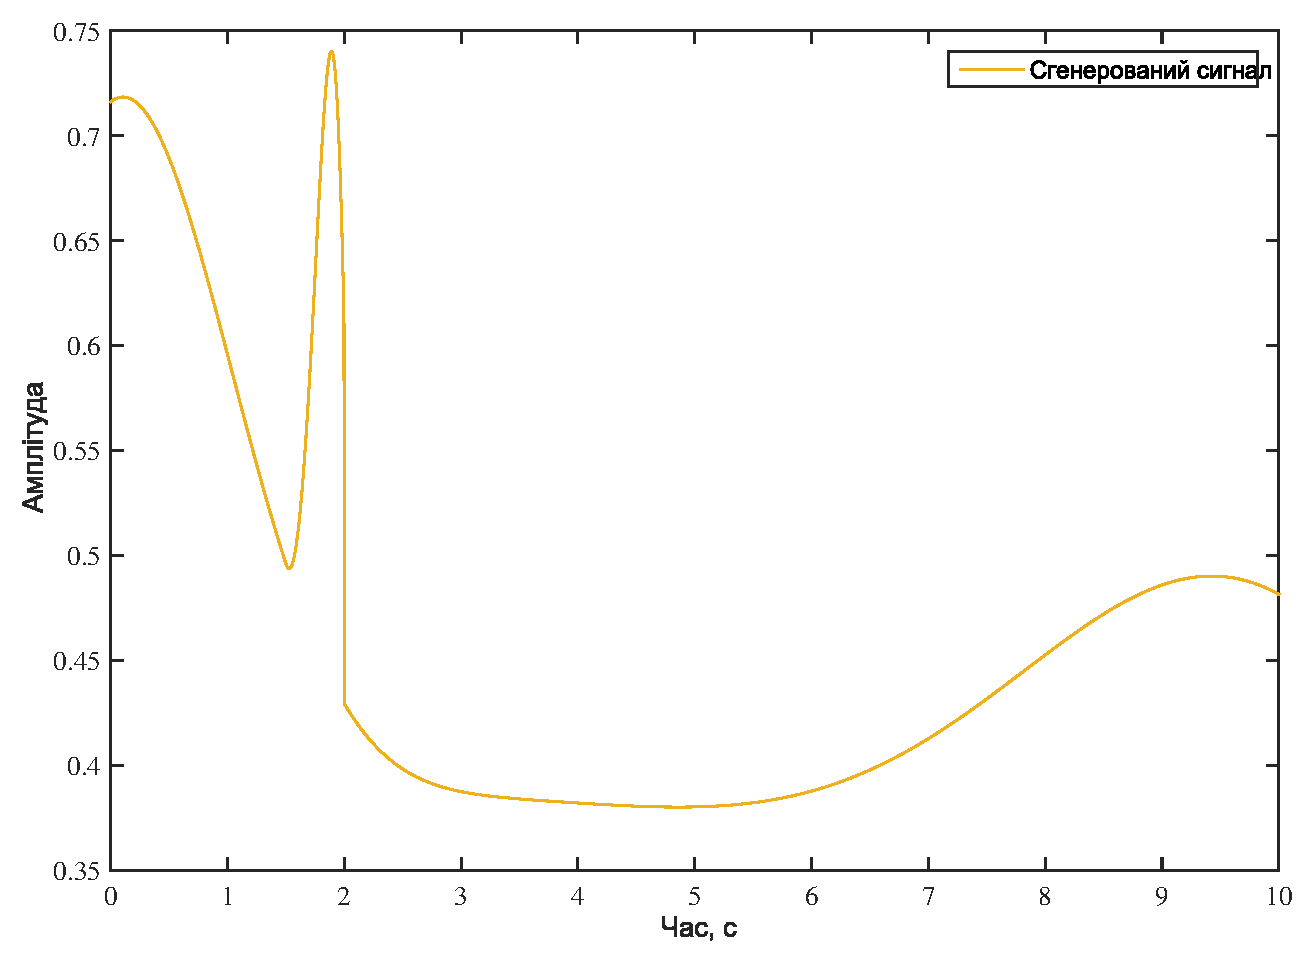
\includegraphics[width=0.8\textwidth]{signal-without-noise.eps}
        }

        \subfloat[Із шумом]{%
            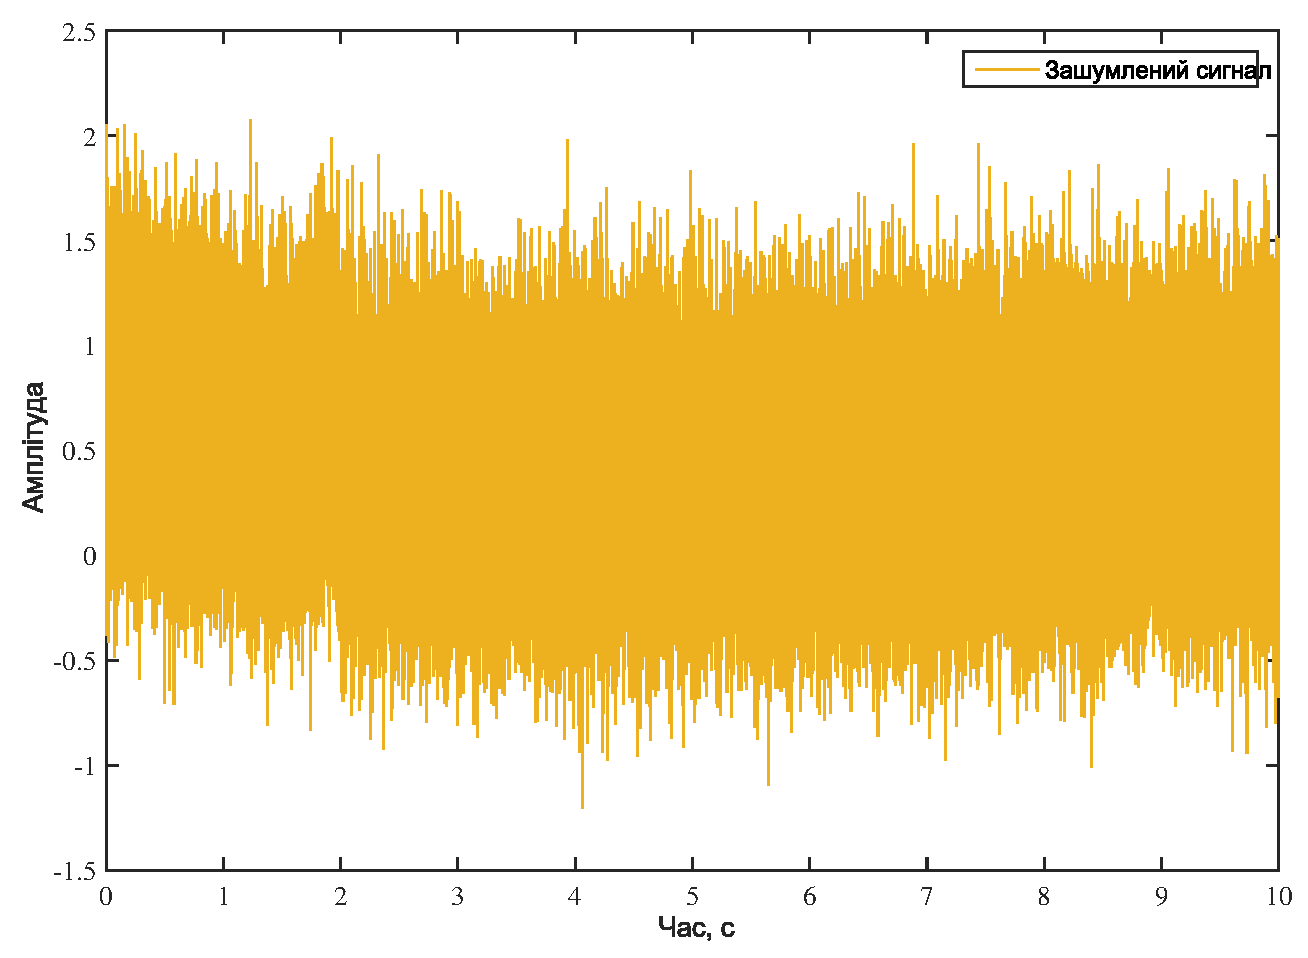
\includegraphics[width=0.8\textwidth]{signal-with-noise.eps}
        }
        \caption{Приклад сигналу із шаблоном без модифікації}
        \label{fig:signal}
    \end{figure}

    \stepcounter{figurecount}
    \begin{figure}[h]
        \centering
        \subfloat[NCC]{%
            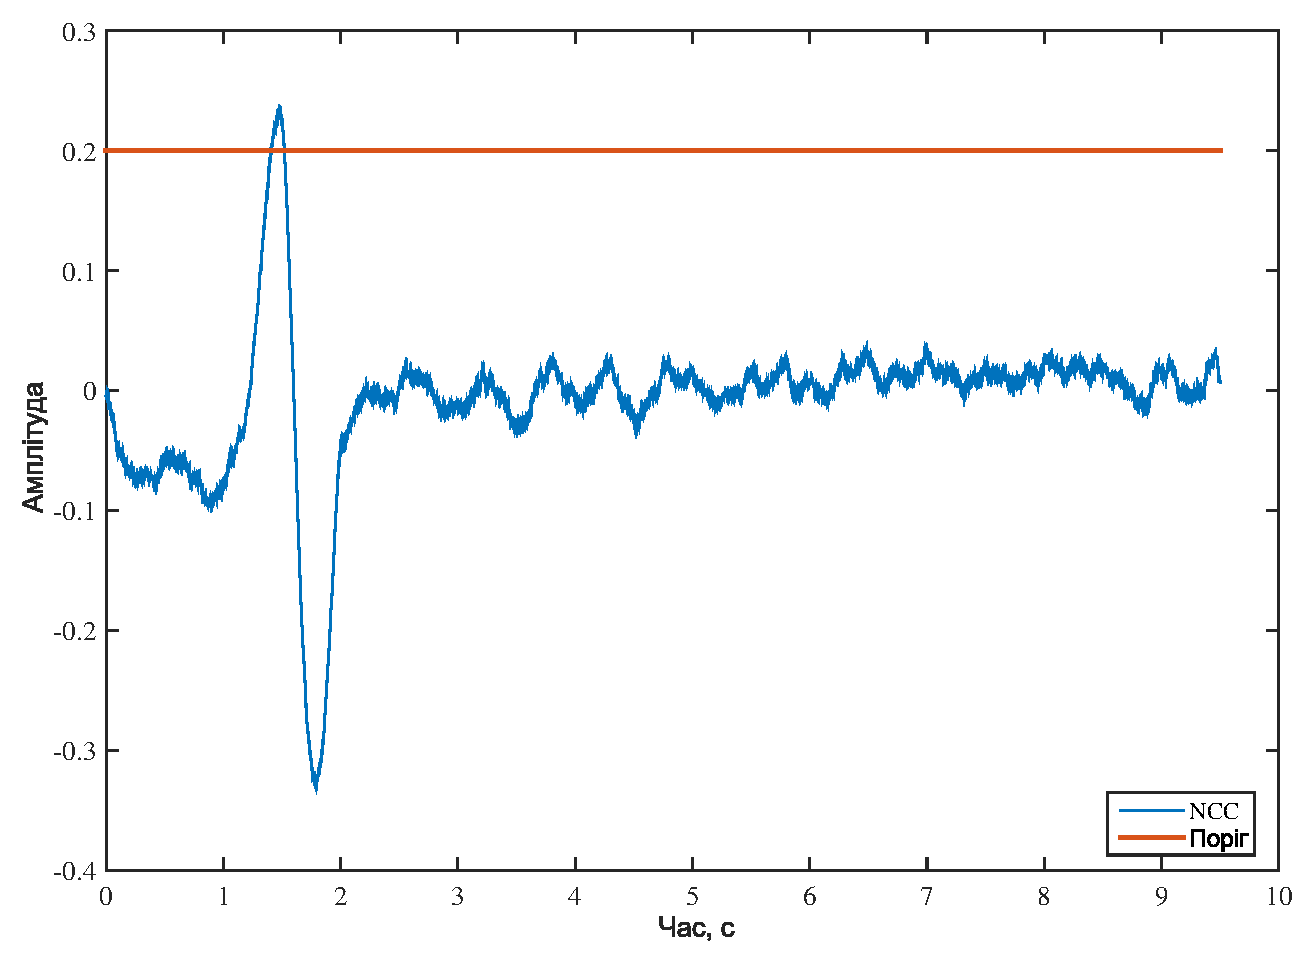
\includegraphics[height=0.28\textheight]{signal-ncc.eps}
        }

        \subfloat[NSSD]{%
            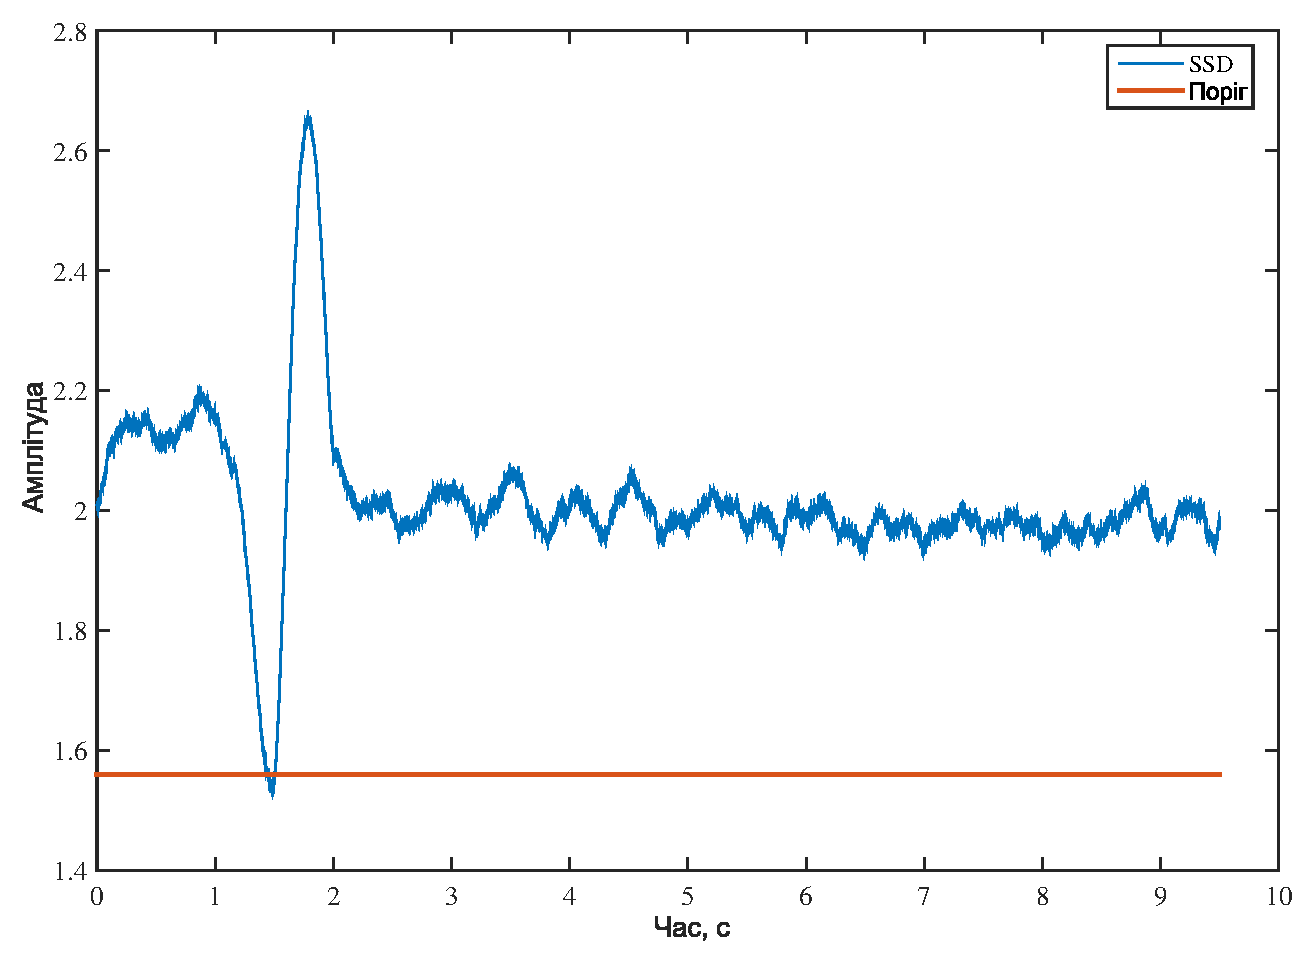
\includegraphics[height=0.28\textheight]{signal-ssd.eps}
        }

        \subfloat[Kunchenko]{%
            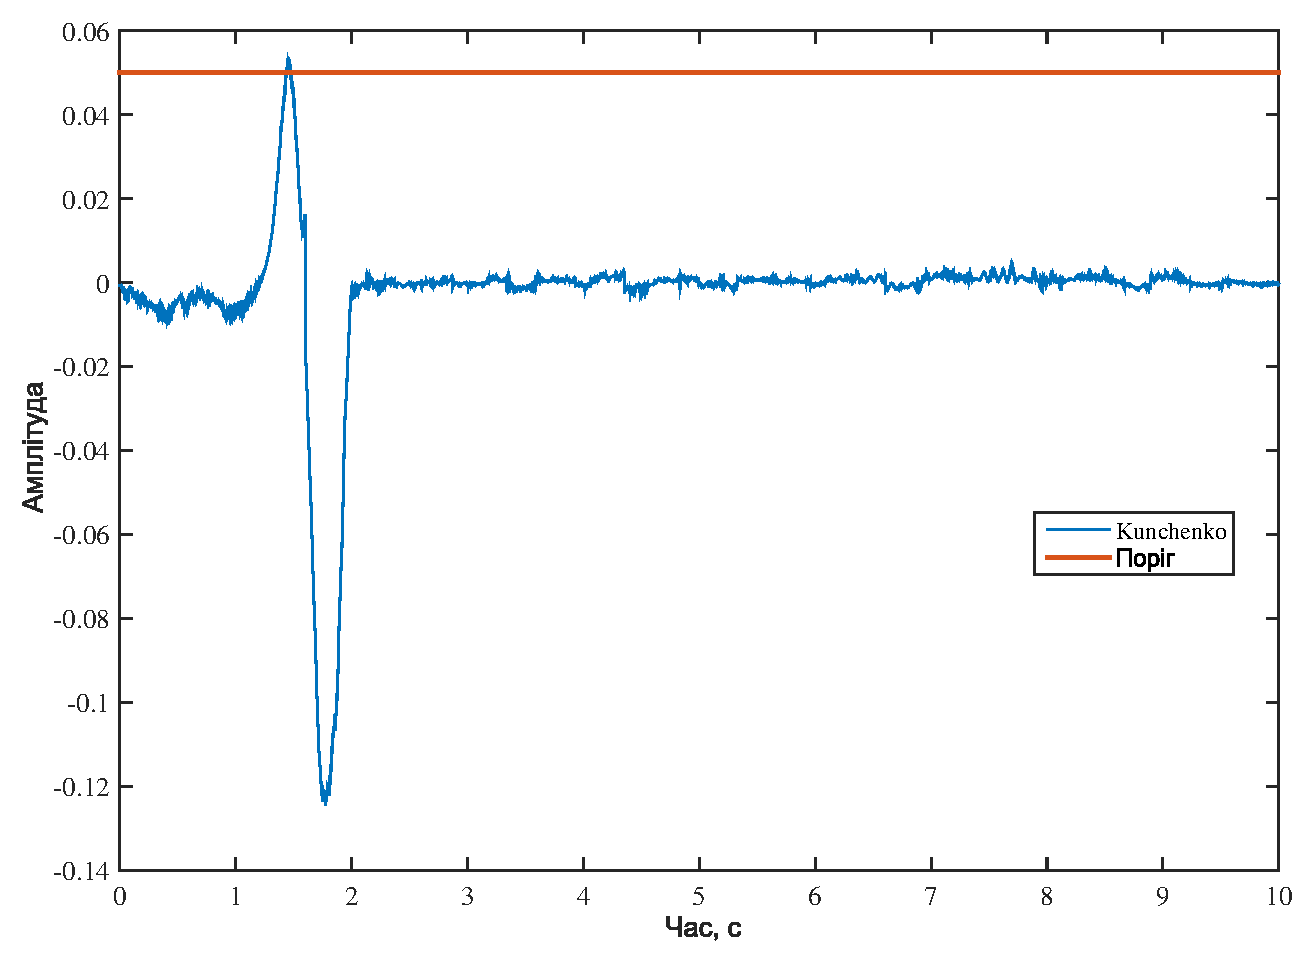
\includegraphics[height=0.28\textheight]{signal-kun.eps}
        }

        \caption{Пошук шаблона без модифікацій в синтетичному сигналі}
        \label{fig:simple-signal}
    \end{figure}

    \stepcounter{figurecount}
    \begin{figure}[h]
        \centering
        \subfloat[Крок 0,01]{%
            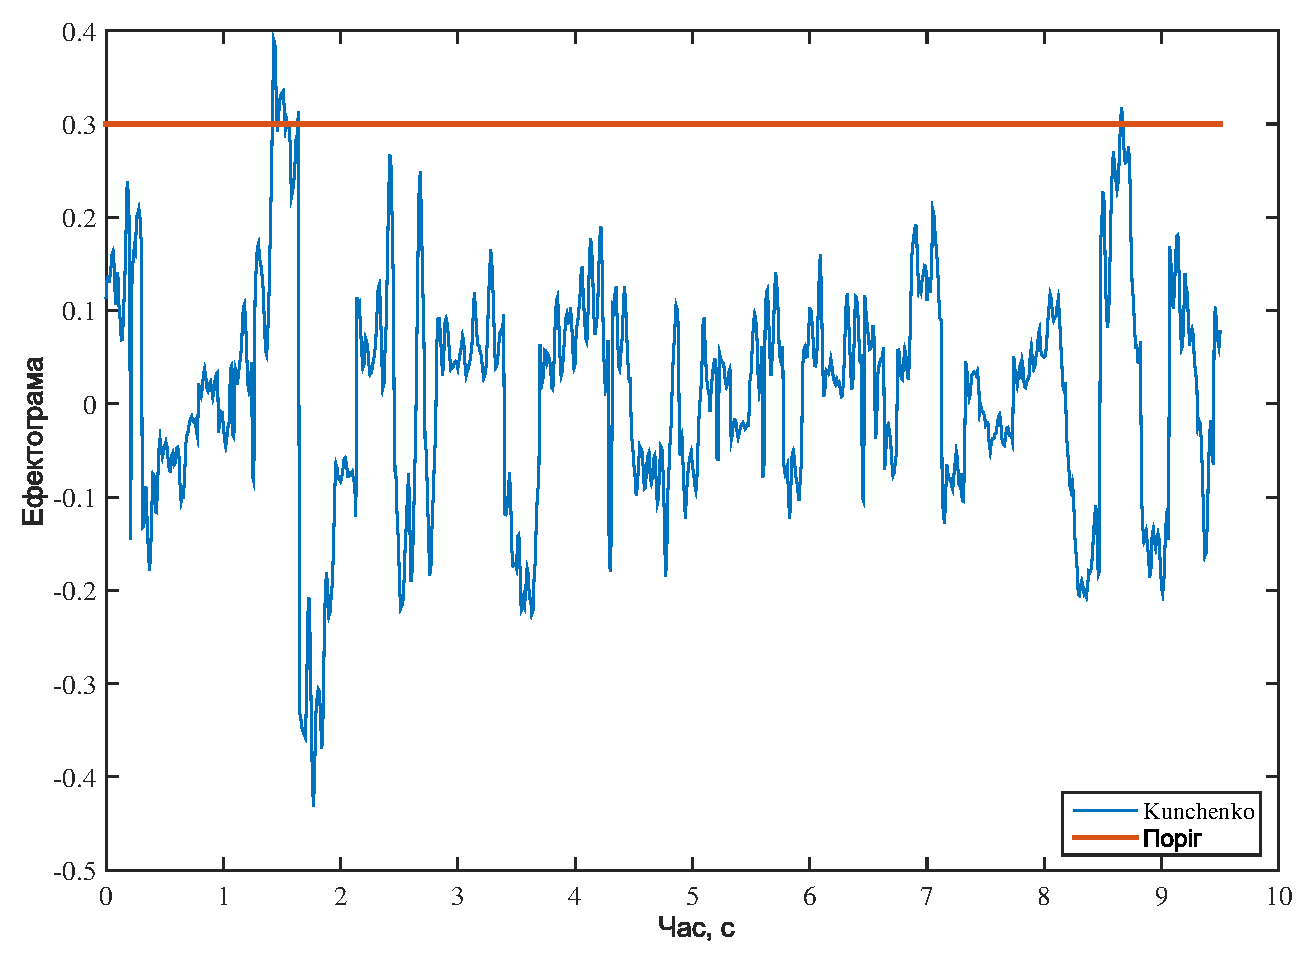
\includegraphics[height=0.28\textheight]{signal-kun-10.eps}
        }

        \subfloat[Крок 0,001]{%
            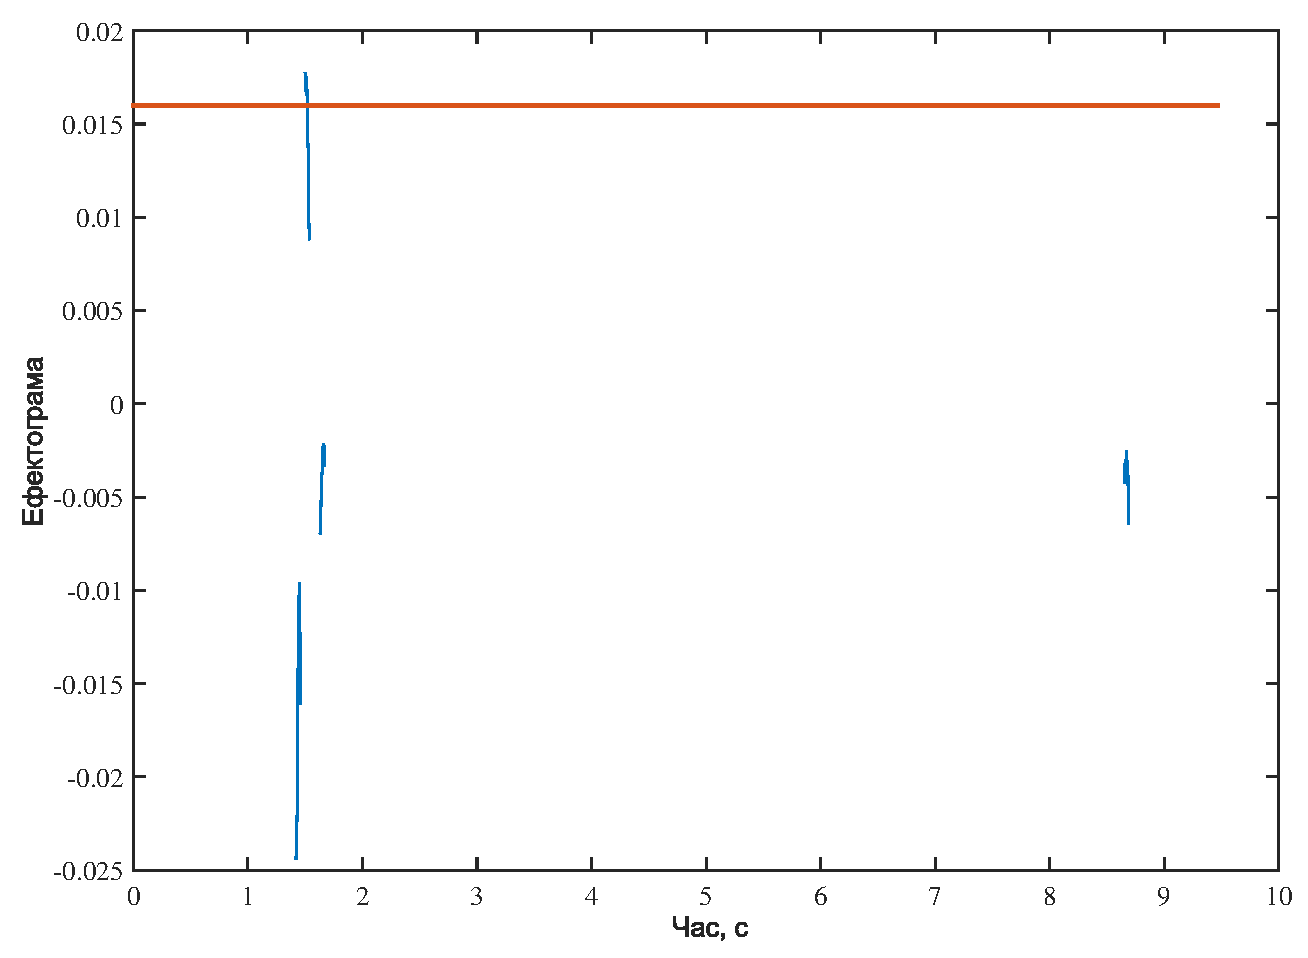
\includegraphics[height=0.28\textheight]{signal-kun-100.eps}
        }

        \subfloat[Крок 0,0001]{%
            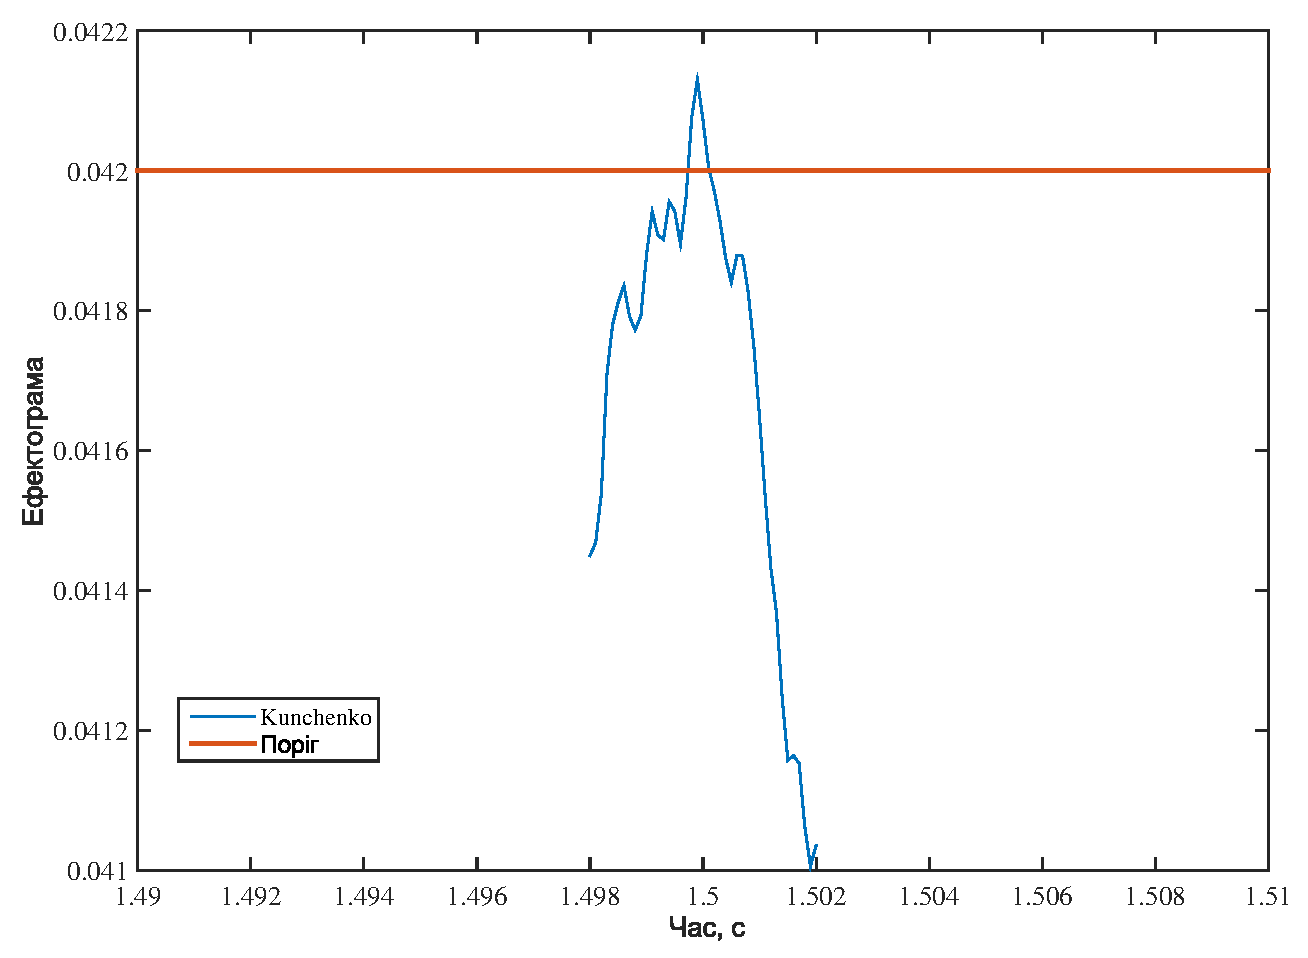
\includegraphics[height=0.28\textheight]{signal-kun-1000.eps}
        }

        \caption{Застосування пірамідального пошуку}
        \label{fig:simple-signal-kun-p}
    \end{figure}
    \clearpage

\section{Пошук шаблону у мовленнєвому сигналі}
    Протестуємо метод Кунченко для пошуку шаблону в мовленнєвому сигналі.

    В якості тестових даних було використано заздалегідь підготовлений акустичний файли, що містили запис озвучення
    ряду цифр.
    В якості шаблонів використовувався записаний аналогічно файл, що містив записи озвучення окремих цифр.

    Таким чином, пошук шаблону повинен був виявити моменту часу в вхідних даних, коли було озвучено ту ж саму цифру,
    що й в шаблоні.

    Як було розглянуто в розділі~\ref{chap:selected}, при обробці мовленнєвих сигналів було запропоновано
    використовувати коротко"=часову енергію.

    При обчисленні коротко"=часової енергії отримане значення буде залежати від довжини вікна, віконної функції та
    кроку між вікнами.
    В експериментах довжина вікна була обрана статичним чином як 20 мілісекунд.

    В експерименті буде проаналізовано залежність ефективності пошуку шаблону розглянутими методами від
    \begin{itemize}
        \item обраного представлення сигналу та шаблону (акустичний сигнал чи коротко"=часова енергія);
            для коротко"=часової енергії ще будуть розглянуті наступні параметри:
            \begin{itemize}
                \item віконна функція, що використовується при обрахунку енергії;
                \item крок між вікнами (мінімальний чи половина вікна);
            \end{itemize}
        \item віконної функції, що використовується у методі ковзного вікна.
    \end{itemize}

    Розглянемо результати тестування для сигналу, що містить озвученим наступний ряд: $1;2;3;4;5;6;1;2;3;1;2;3$.
    В якості шаблону розглядатимемо аудіозапис, що містить озвученої цифру 1.
    В сигналі, що розглядається, цифра 1 вимовляється приблизно на 0,5, 5 та 7 секундах.

    \subsection{Пошук шаблону в аудіосигналі}
        На рисунку~\ref{fig:audio} на сторінці~\pageref{fig:audio} наведено вигляд аудіосигналів.

        На рисунках~\ref{fig:audio-plain-rect},~\ref{fig:audio-plain-hamming} та~\ref{fig:audio-plain-hanning} на
        сторінках~\pageref{fig:audio-plain-rect},~\pageref{fig:audio-plain-hamming}
        та~\pageref{fig:audio-plain-hanning} відповідно, зображено результати пошуку шаблону в аудіосигналі.

        З цих результатів видно, що використання жодного з методів не дозволило знайти усі входження шаблонів в
        сигналі.
        З цих результатів можна зробити наступні спостереження:
        \begin{itemize}
            \item Екстремуми, що відповідають коректним позиціям шаблону в сигналі, при використанні методу поліномів
                Кунченка, як правило, є більш вираженими ніж у інших методів.
            \item Використання вікон, відмінних від прямокутного значно зменшує амплітуду ефектограм в зонах, що не
                містять шаблону.
                В цих зонах все ще є певні екстремуми, але вони стають більш вираженими.
            \item Метод сум квадратів відстаней при використанні вікон, відмінних від прямокутних, має тільки один
                коректний екстремум, менший за поріг.
        \end{itemize}

        \stepcounter{figurecount}
        \begin{figure}[h]
            \centering
            \subfloat[Сигнал]{%
                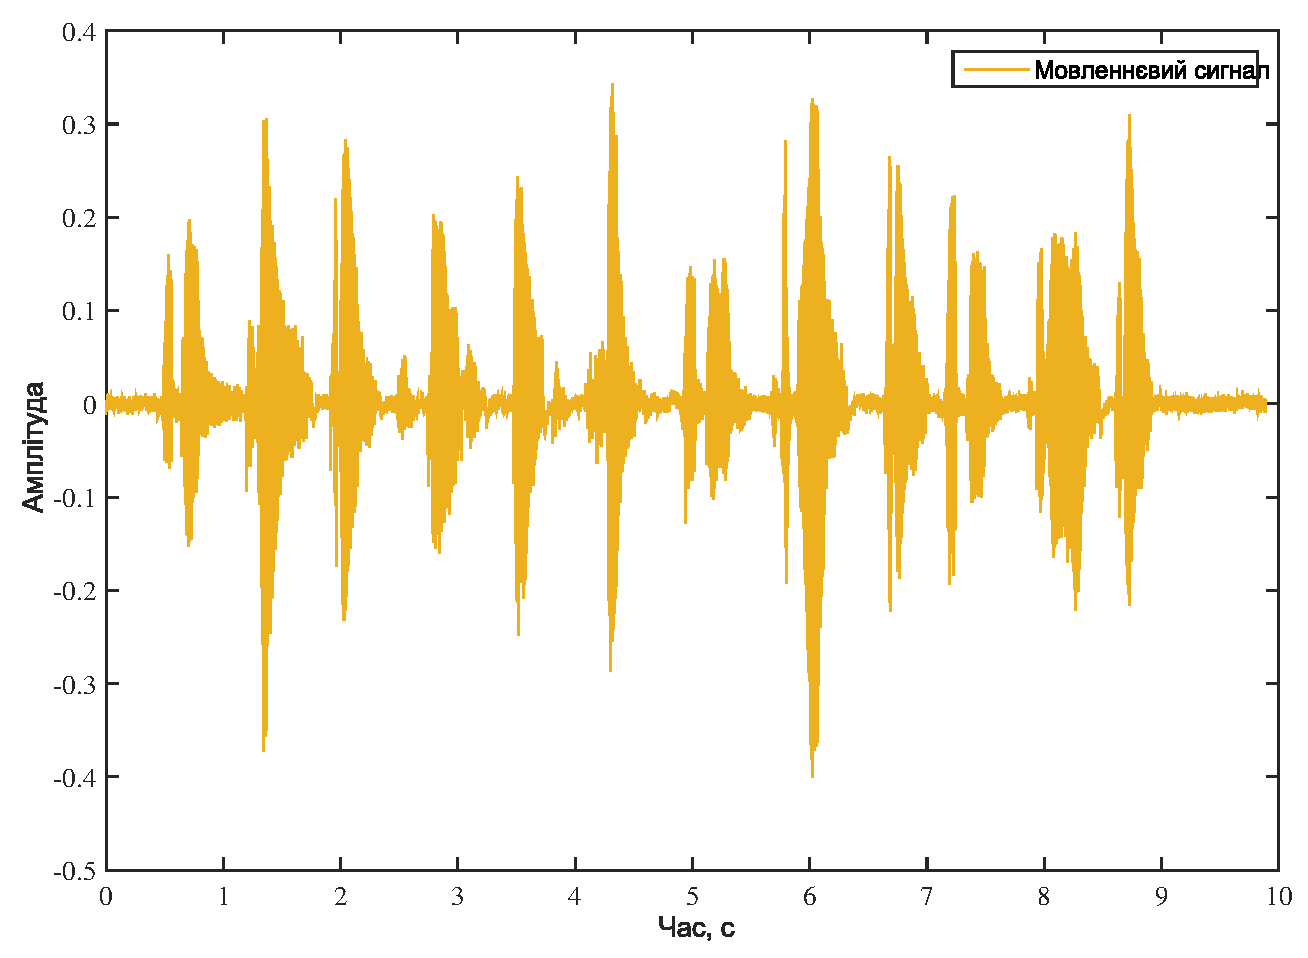
\includegraphics[width=0.8\textwidth]{audio.eps}
            }

            \subfloat[Зразок]{%
                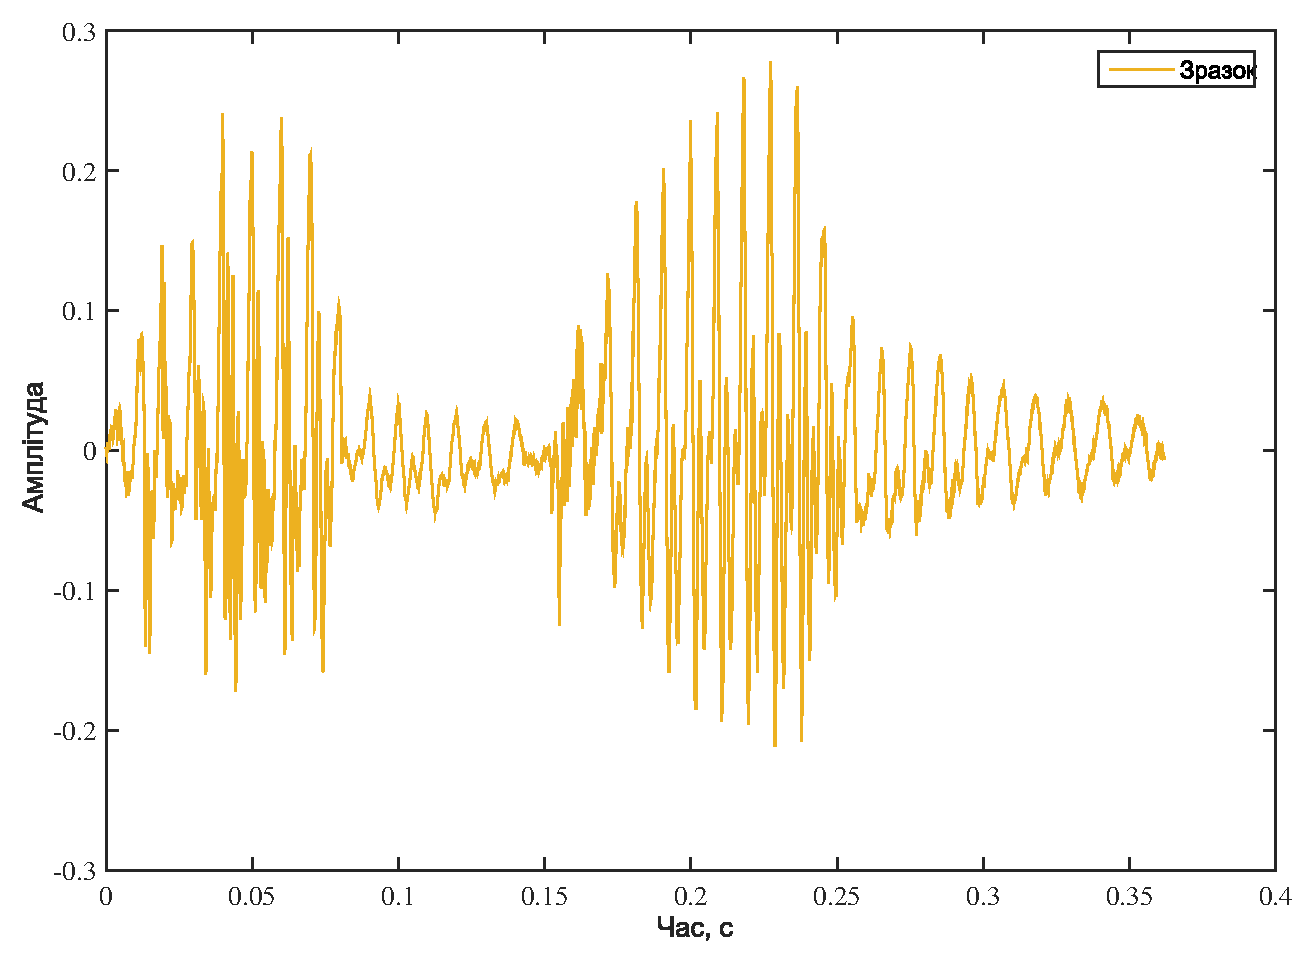
\includegraphics[width=0.8\textwidth]{audio_template.eps}
            }
            \caption{Запис мовлення й шаблон для пошуку}
            \label{fig:audio}
        \end{figure}

        \stepcounter{figurecount}
        \begin{figure}[h]
            \centering
            \subfloat[NCC]{%
                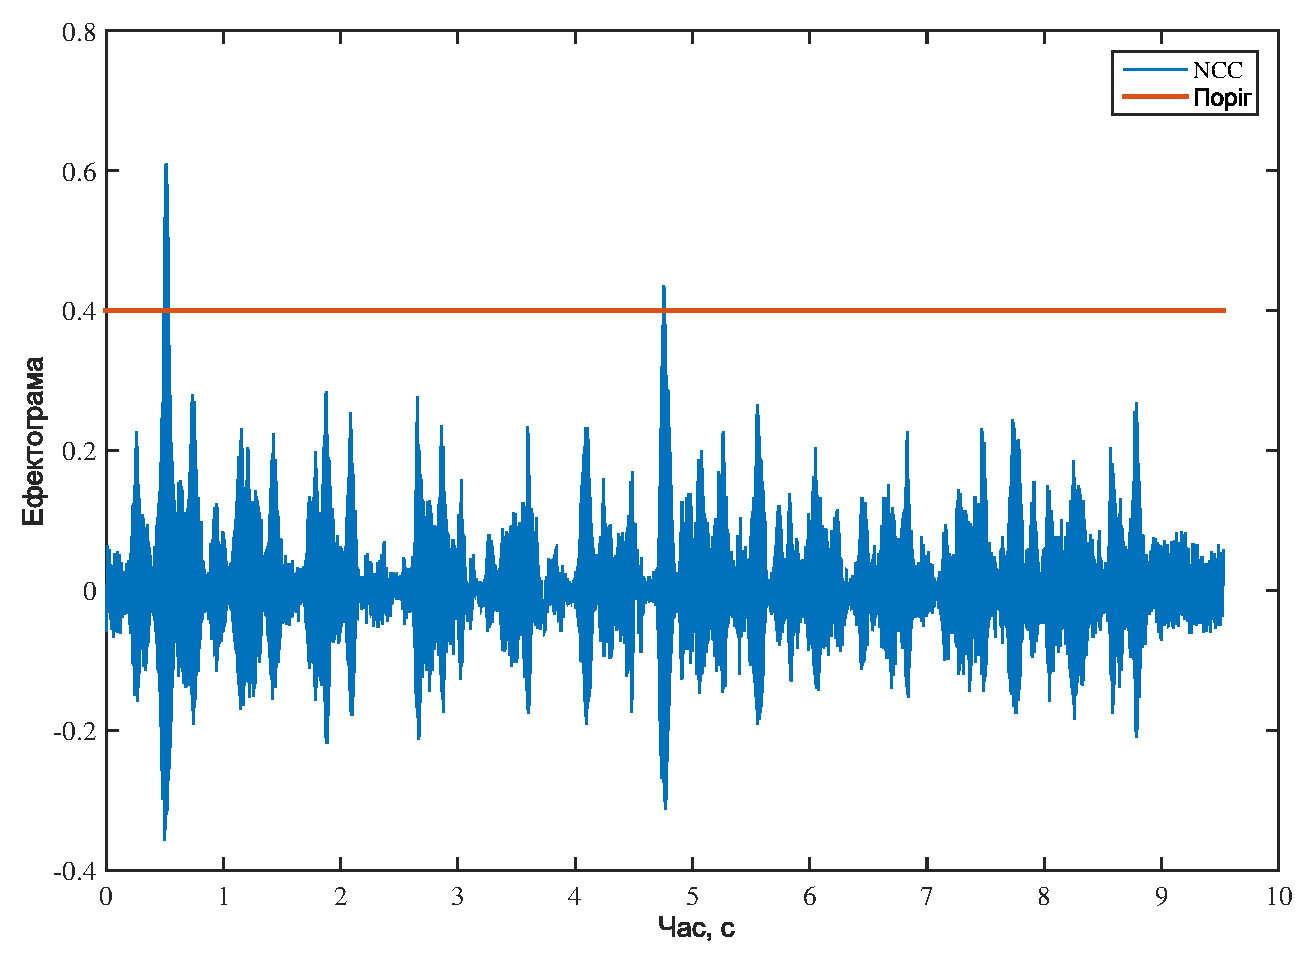
\includegraphics[height=0.28\textheight]{audio-plain-ncc-rect.eps}
            }
            % Час: 2.95

            \subfloat[NSSD]{%
                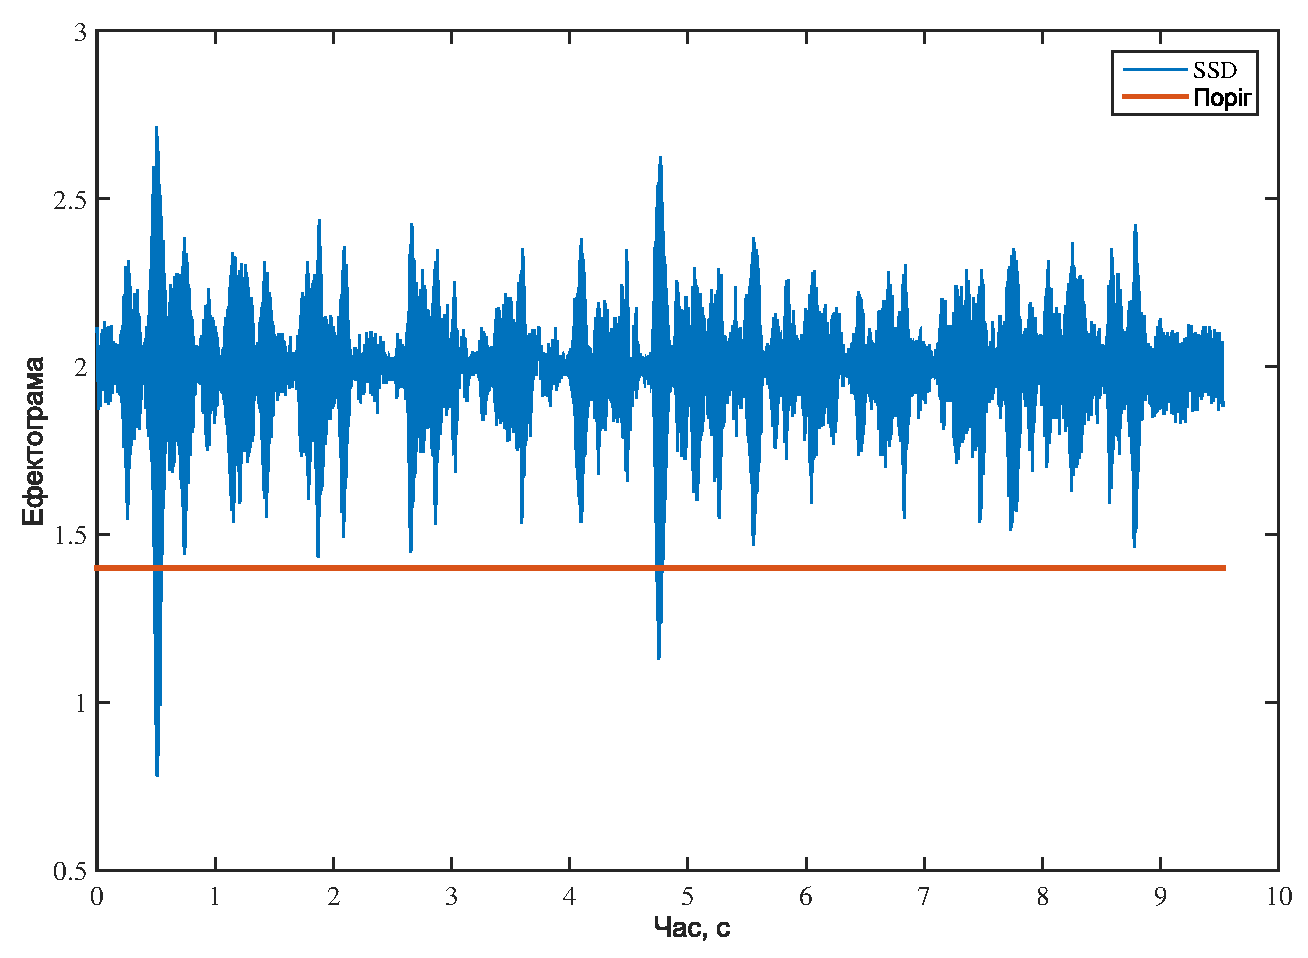
\includegraphics[height=0.28\textheight]{audio-plain-ssd-rect.eps}
            }
            % Час: 2.69

            \subfloat[Kunchenko]{%
                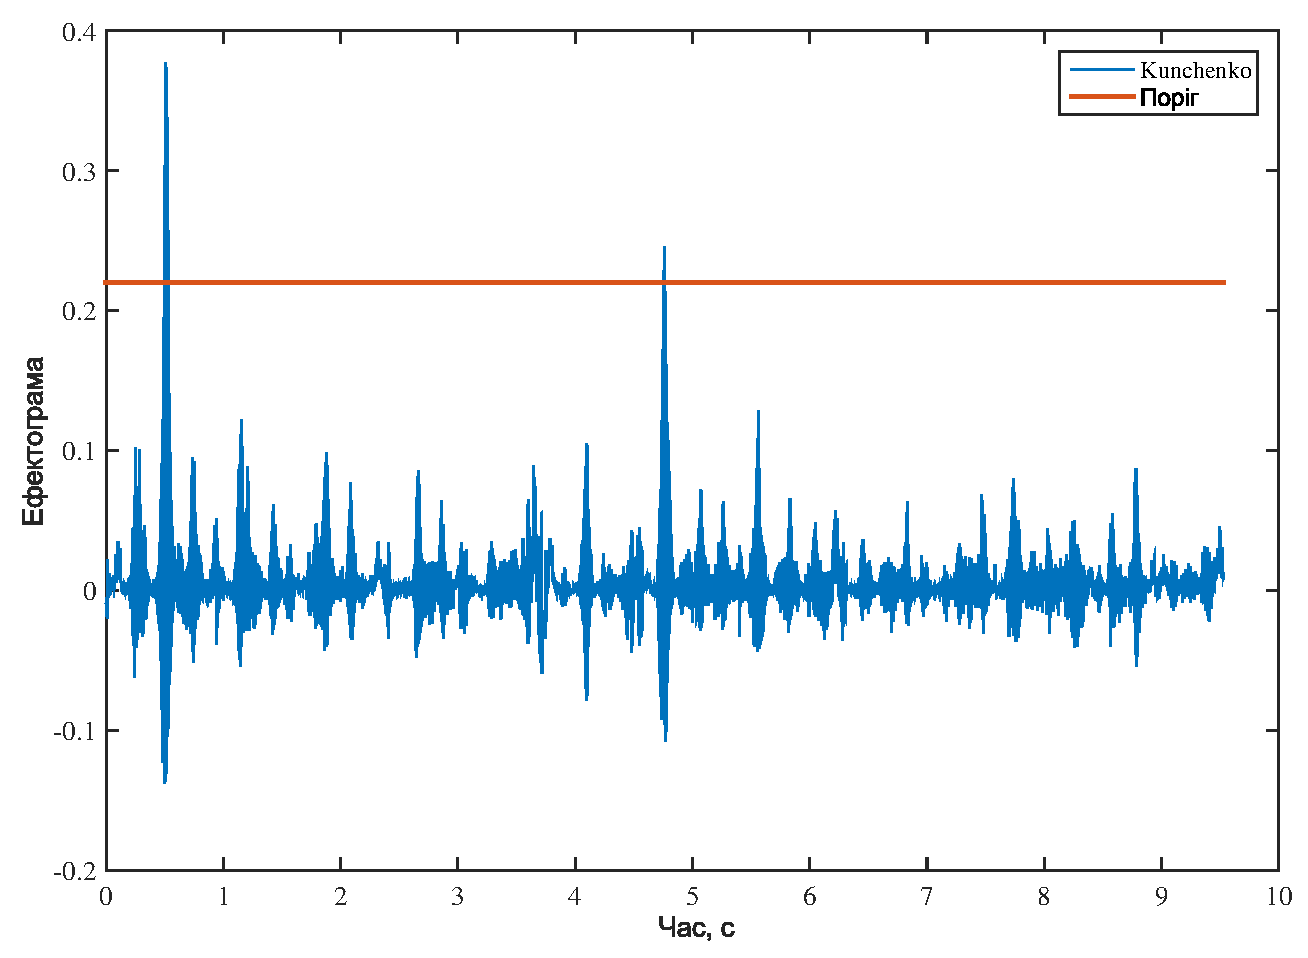
\includegraphics[height=0.28\textheight]{audio-plain-kun-rect.eps}
            }
            % 99.84
            \caption{Результати пошуку шаблону використовуючи прямокутне вікно}
            \label{fig:audio-plain-rect}
        \end{figure}

        \stepcounter{figurecount}
        \begin{figure}[h]
            \centering
            \subfloat[NCC]{%
                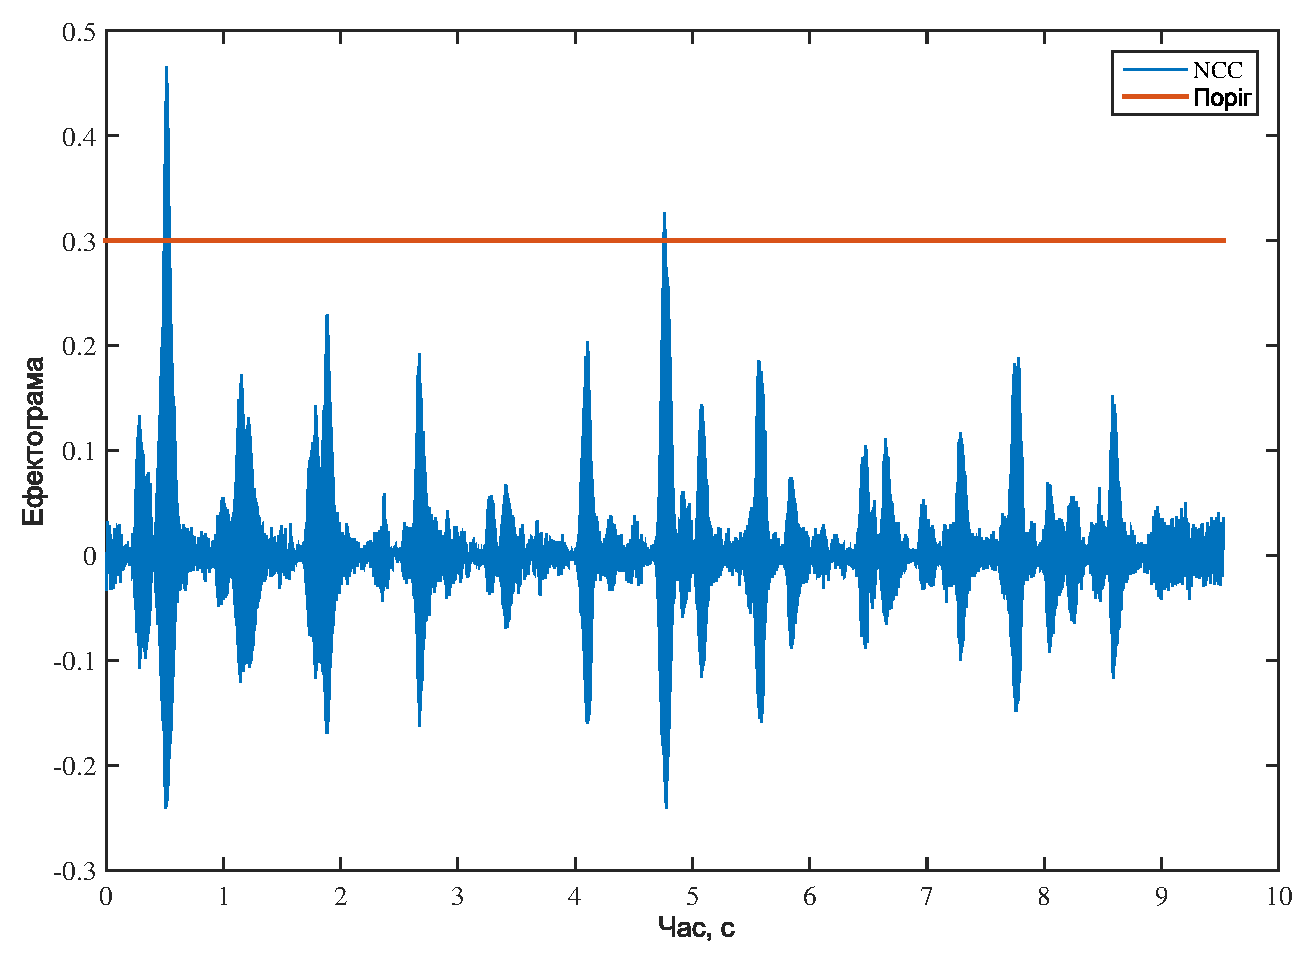
\includegraphics[height=0.28\textheight]{audio-plain-ncc-hamming.eps}
            }
            % Час: 3.67


            \subfloat[NSSD]{%
                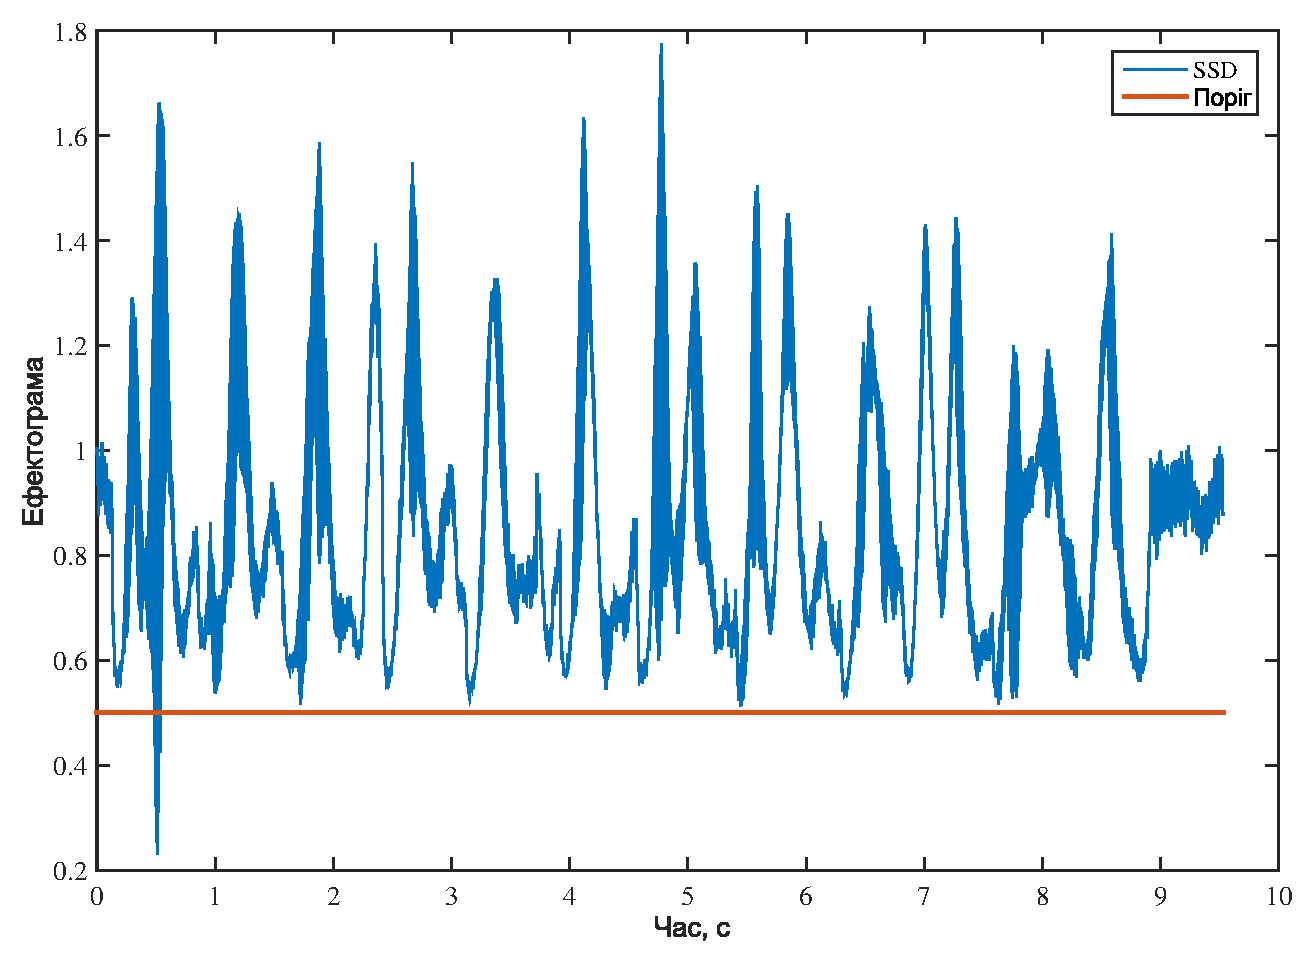
\includegraphics[height=0.28\textheight]{audio-plain-ssd-hamming.eps}
            }
            % Час: 3.45

            \subfloat[Kunchenko]{%
                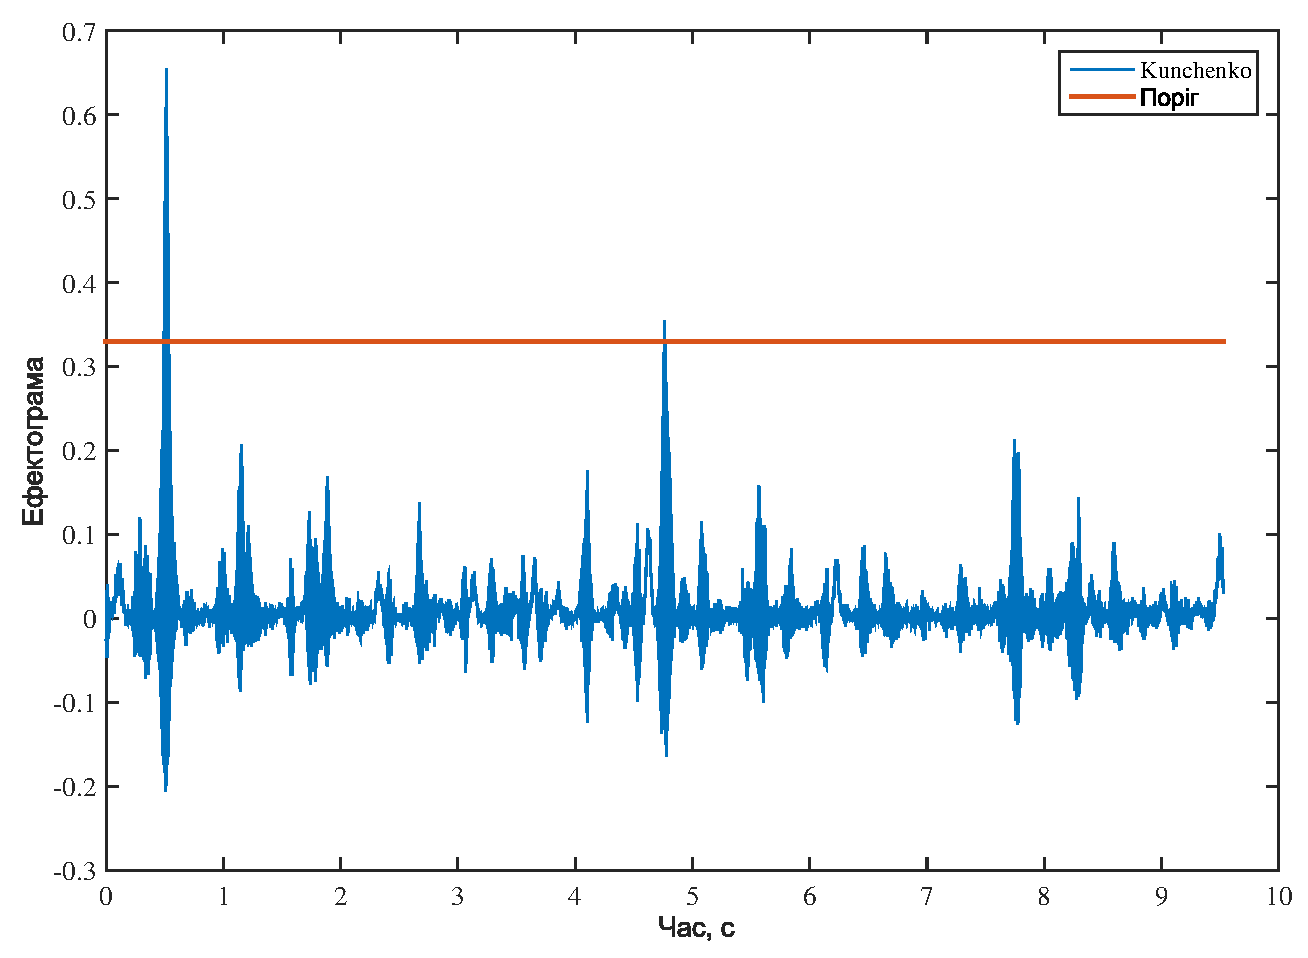
\includegraphics[height=0.28\textheight]{audio-plain-kun-hamming.eps}
            }
            % 133.20
            %
            \caption{Результати пошуку шаблону використовуючи вікно Геммінга}
            \label{fig:audio-plain-hamming}
        \end{figure}

        \stepcounter{figurecount}
        \begin{figure}[h]
            \centering
            \subfloat[NCC]{%
                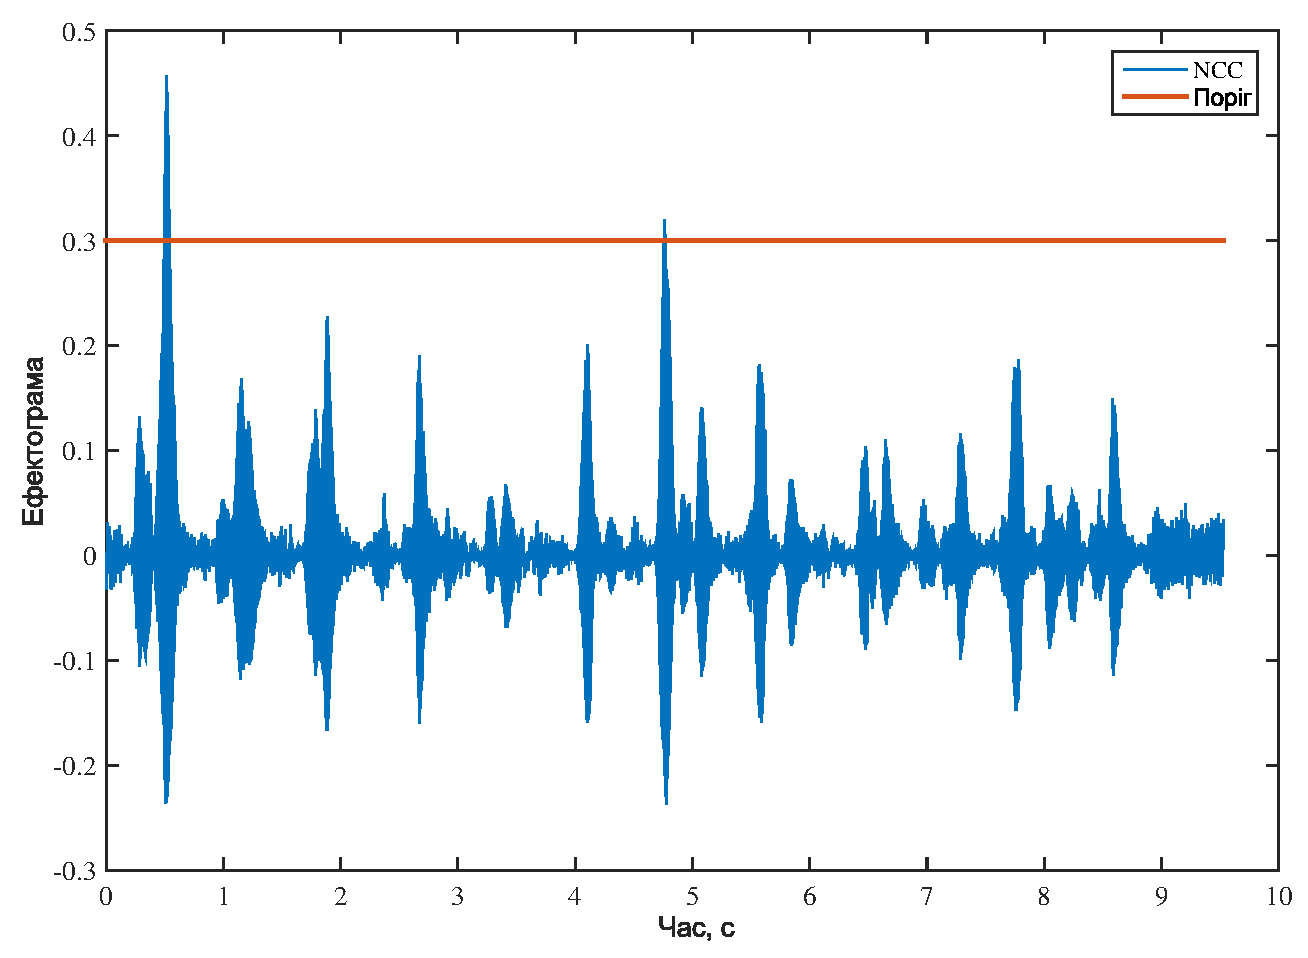
\includegraphics[height=0.28\textheight]{audio-plain-ncc-hann.eps}
            }
            % Час: 3.52

            \subfloat[NSSD]{%
                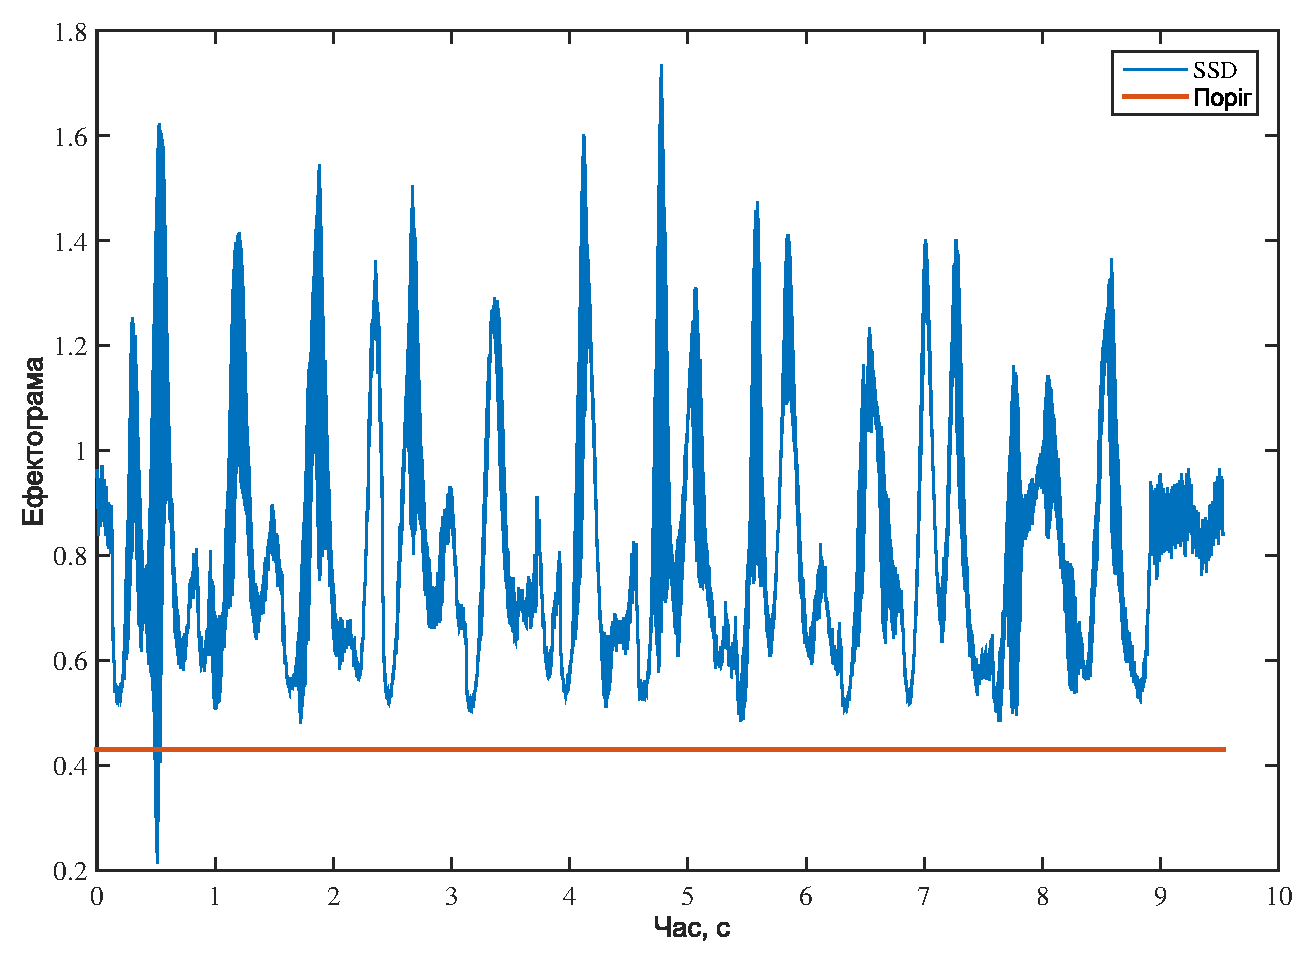
\includegraphics[height=0.28\textheight]{audio-plain-ssd-hann.eps}
            }
            % Час: 3.56

            \subfloat[Kunchenko]{%
                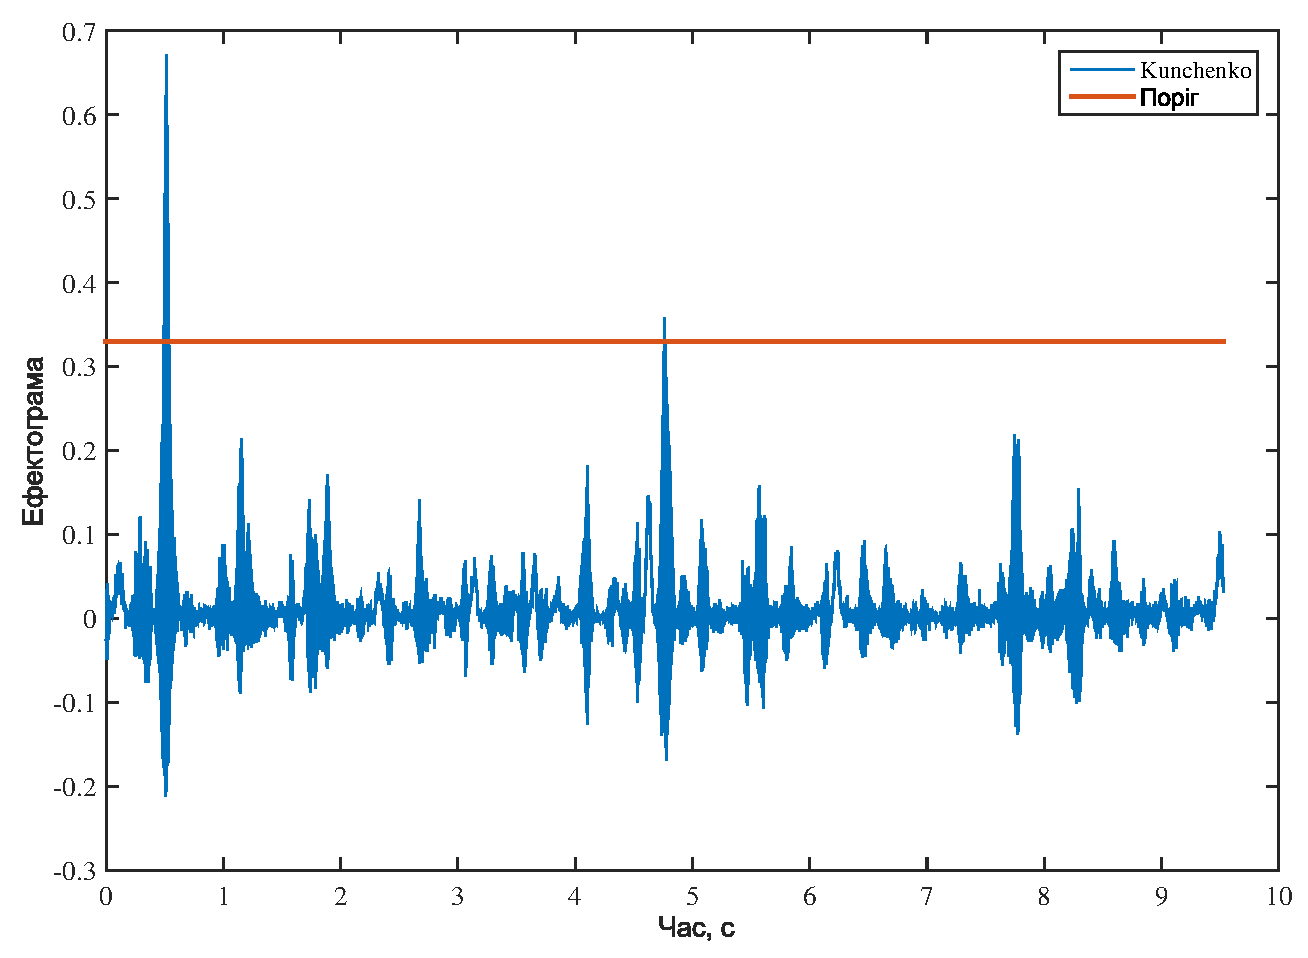
\includegraphics[height=0.28\textheight]{audio-plain-kun-hann.eps}
            }
            % 136.05
            \caption{Результати пошуку шаблону використовуючи вікно Гана}
            \label{fig:audio-plain-hanning}
        \end{figure}
        \clearpage
    \subsection{Пошук шаблону в коротко"=часовій енергії}
        Розглянемо поведінку розглянутих алгоритмів для пошуку шаблонів в коротко"=часовій енергії сигналу, що
        була отримана з використанням найпростішого й найшвидшого методу виділення вікон --- прямокутні вікна.
        Такі вікна бралися з мінімально можливим кроком --- кроком дискретизації.

        На рисунку~\ref{fig:audio-energy-rect-min} на сторінці~\pageref{fig:audio-energy-rect-min} наведений
        вигляд коротко"=часової енергії шаблону та сигналу, що були отримані вказаним способом.

        На рисунках~\ref{fig:matched-energy-rect-min-rect},~\ref{fig:matched-energy-rect-min-hann}
        та~\ref{fig:matched-energy-rect-min-hamming} на
        сторінках~\pageref{fig:matched-energy-rect-min-rect},~\pageref{fig:matched-energy-rect-min-hann}
        та~\pageref{fig:matched-energy-rect-min-hamming} відповідно, зображено результати пошуку шаблону в
        аудіосигналі.

        З цих результатів видно, що усі з розглянутих методів мали дуже багато хибних спрацювань,
        а отже використання прямокутного вікна з мінімальним кроком не є доцільним при підрахунку коротко"=часової
        енергії.

        \stepcounter{figurecount}
        \begin{figure}[h]
            \centering
            \subfloat[Сигнал]{%
                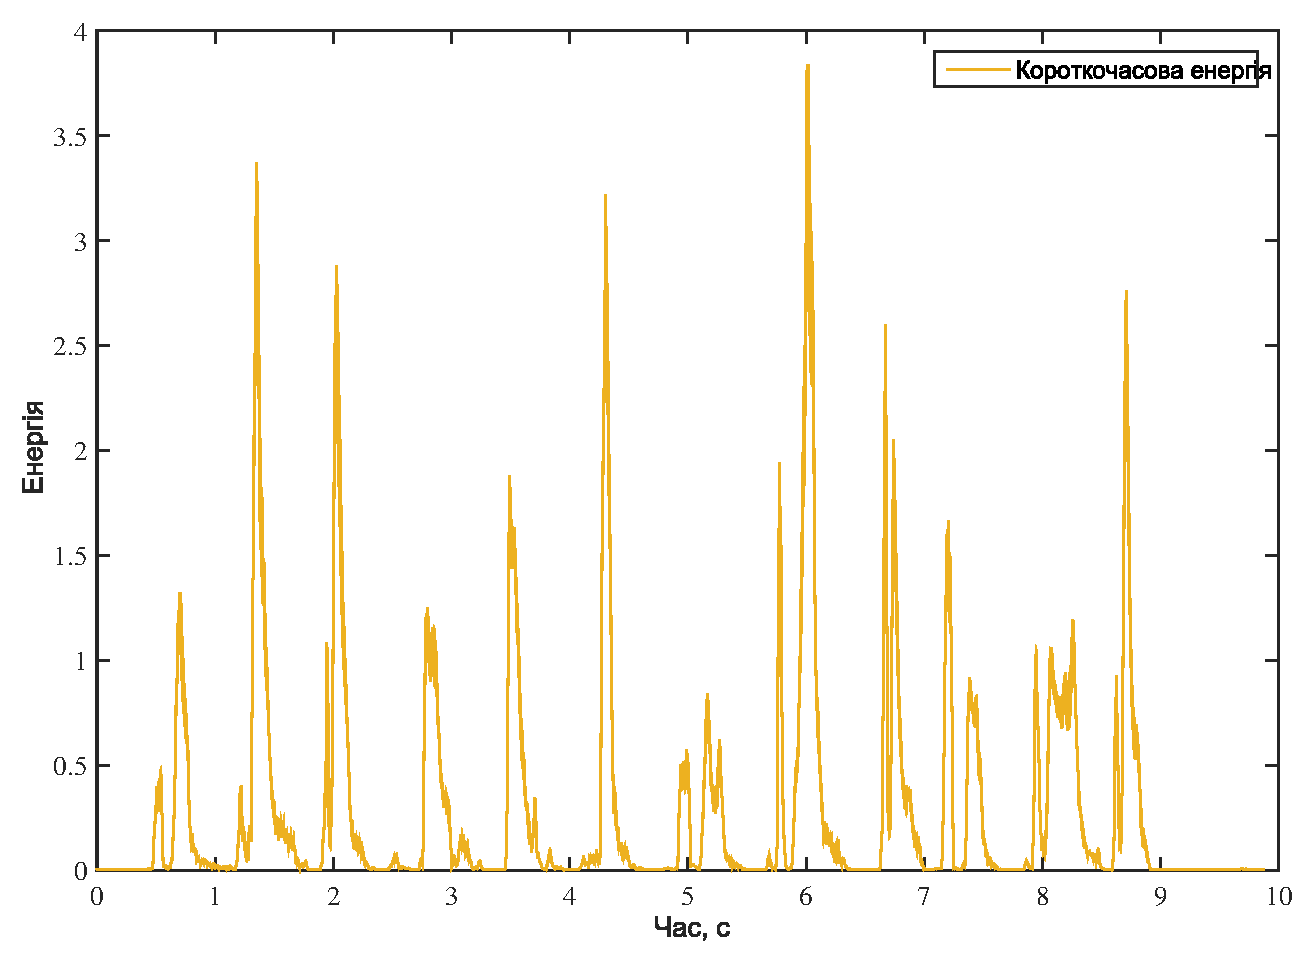
\includegraphics[width=0.8\textwidth]{audio_energy_rect_min.eps}
            }

            \subfloat[Зразок]{%
                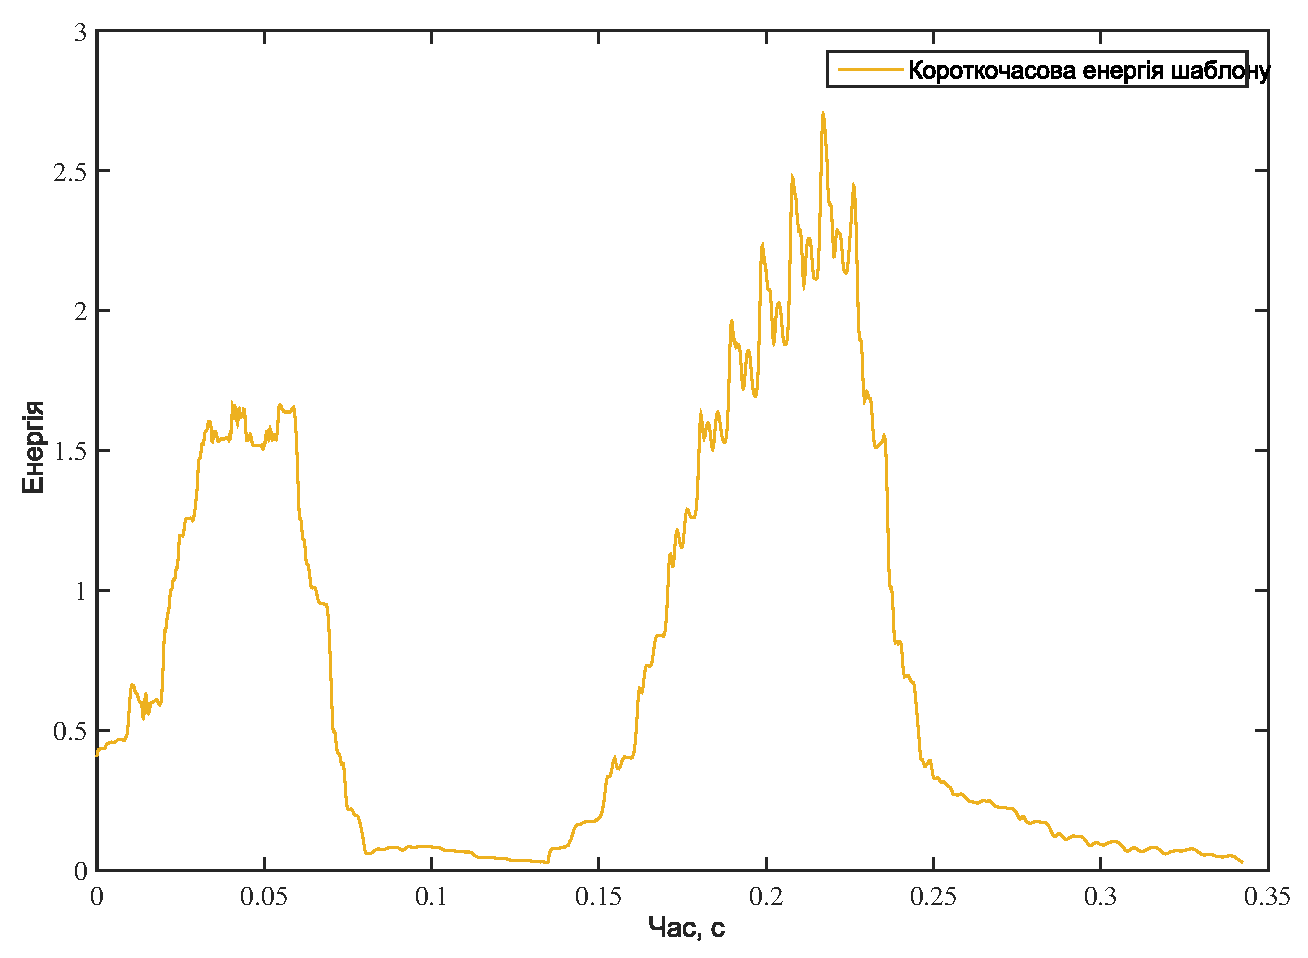
\includegraphics[width=0.8\textwidth]{audio_t_energy_rect_min.eps}
            }
            \caption{Короткочасна енергія запису мовлення й шаблону для пошуку використовуючи прямокутне вікно та
                мінімальний крок}
            \label{fig:audio-energy-rect-min}
        \end{figure}

        \stepcounter{figurecount}
        \begin{figure}[h]
            \centering
            \subfloat[NCC]{%
                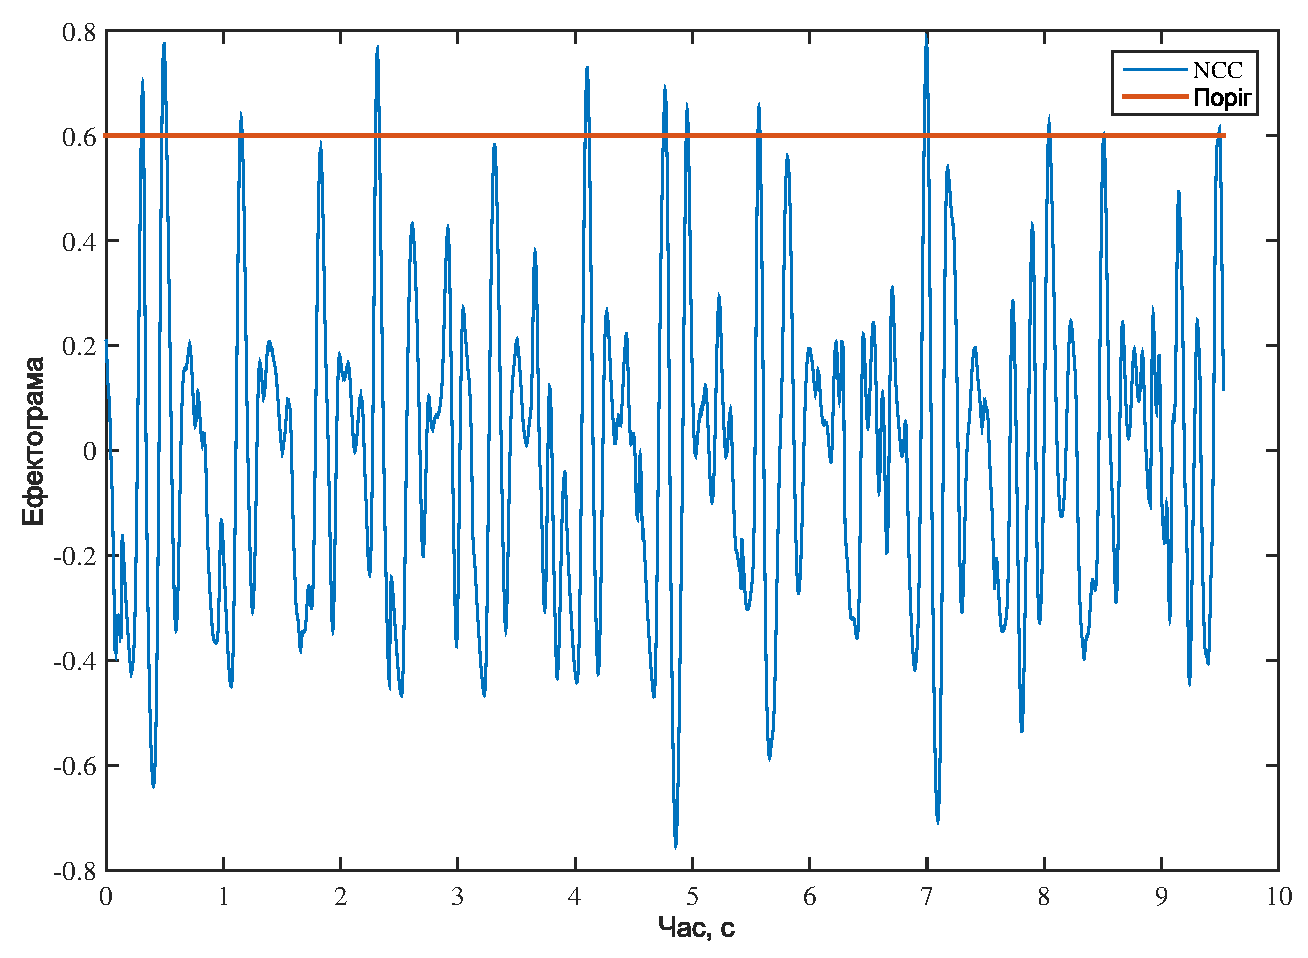
\includegraphics[height=0.28\textheight]{audio-energy-rect-min-ncc-rect.eps}
            }
            % 2.55

            \subfloat[NSSD]{%
                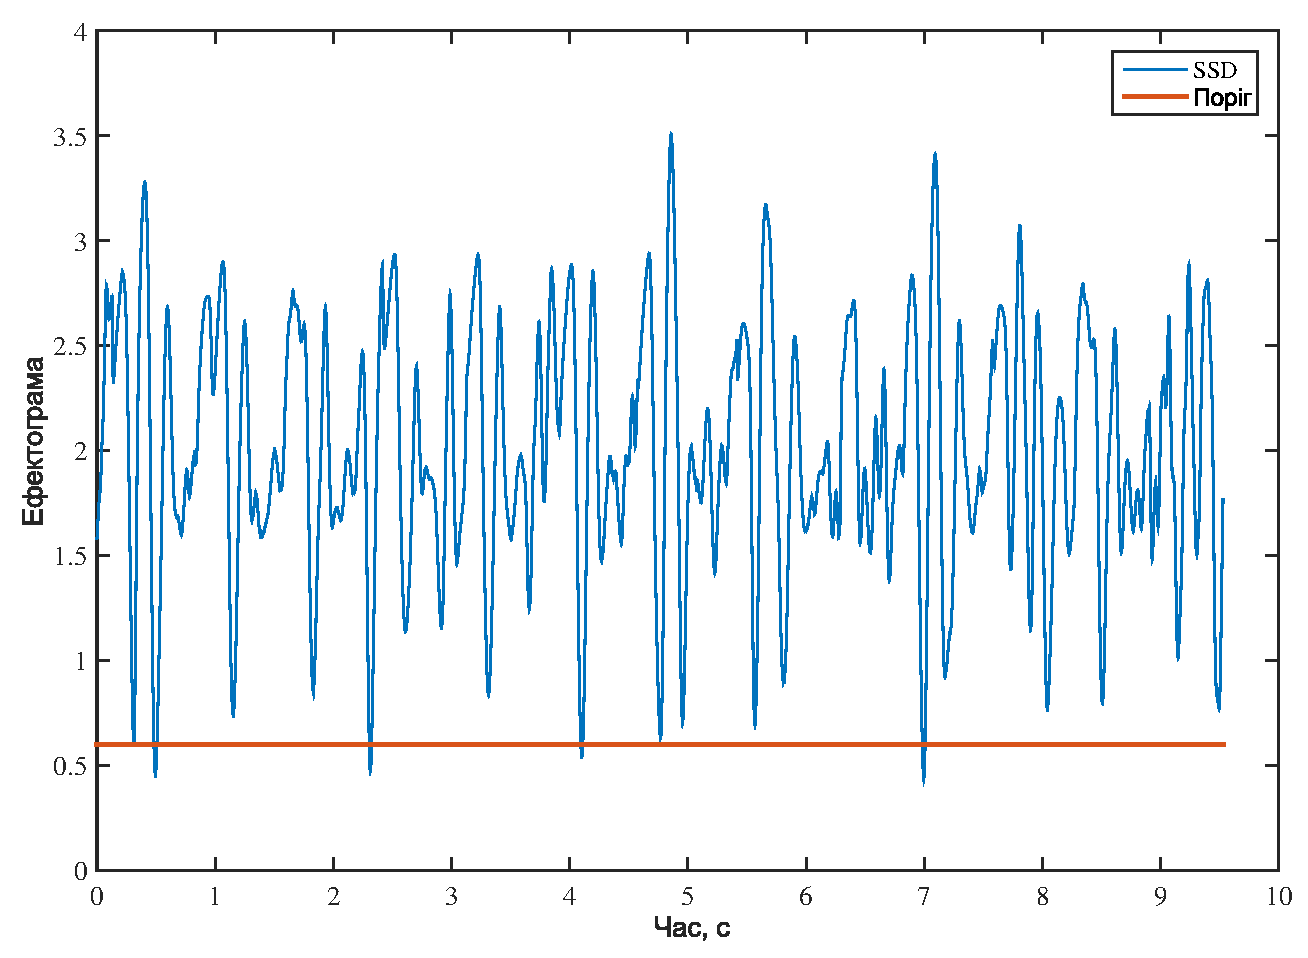
\includegraphics[height=0.28\textheight]{audio-energy-rect-min-ssd-rect.eps}
            }
            % 2.61

            \subfloat[Kunchenko]{%
                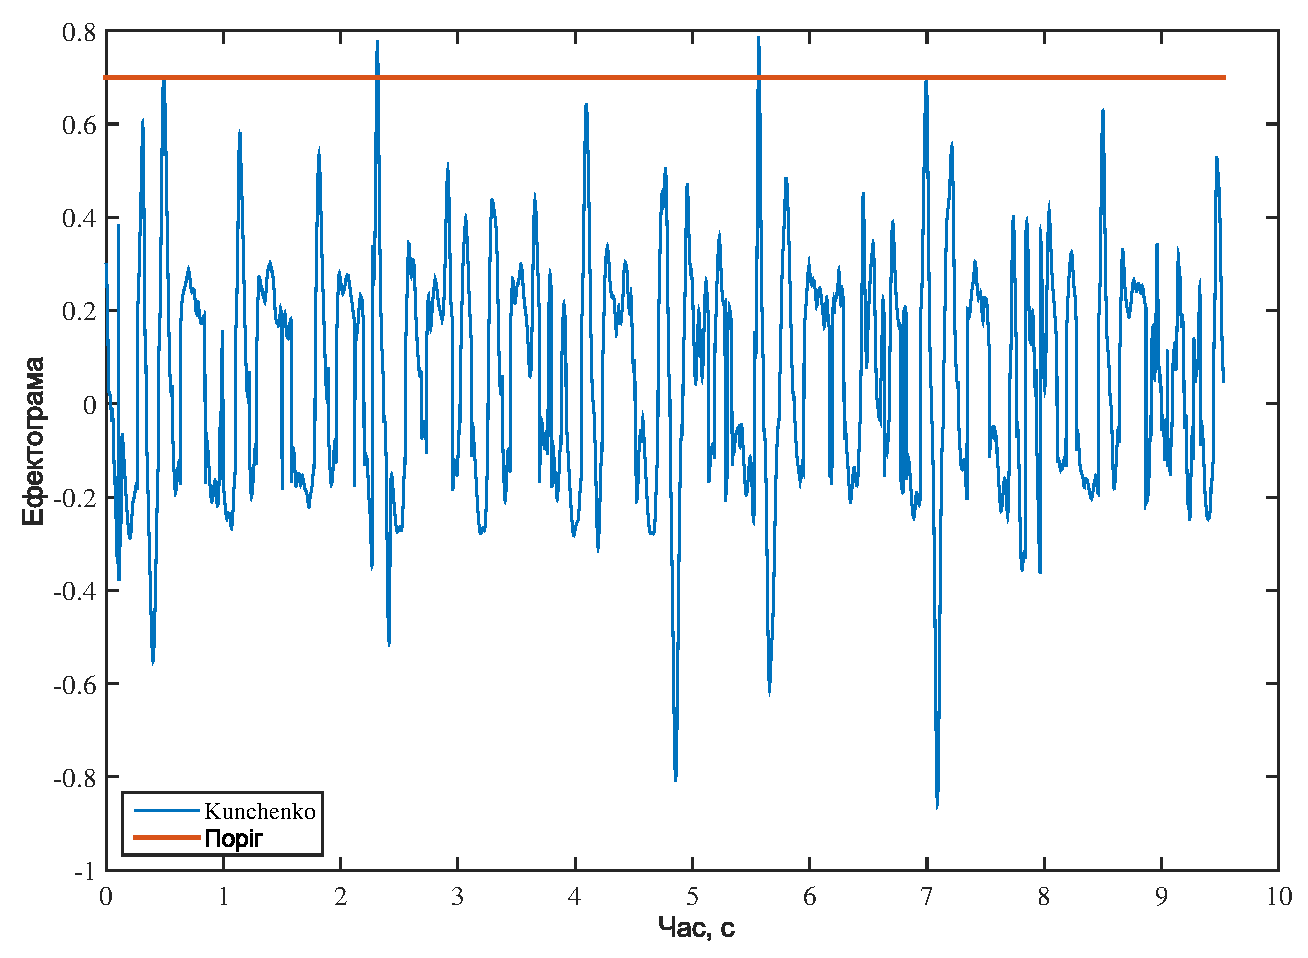
\includegraphics[height=0.28\textheight]{audio-energy-rect-min-kun-rect.eps}
            }
            % 94.68

            \caption{Знайдений шаблон в енергії, наведеної на рисунку~\ref{fig:audio-energy-rect-min},
                використовуючи прямокутні вікна}
            \label{fig:matched-energy-rect-min-rect}
        \end{figure}

        \stepcounter{figurecount}
        \begin{figure}[h]
            \centering
            \subfloat[NCC]{%
                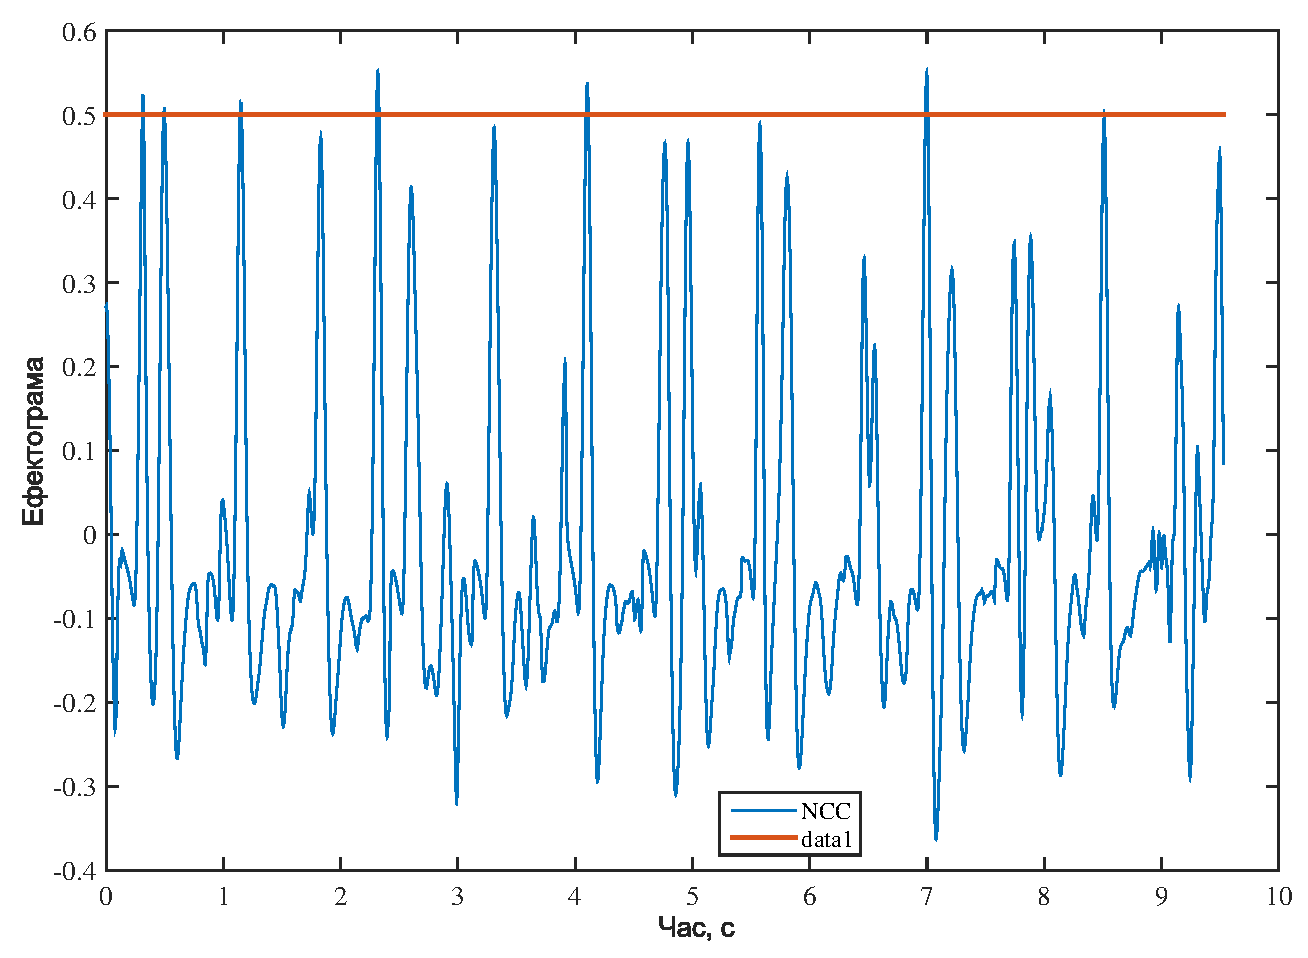
\includegraphics[height=0.28\textheight]{audio-energy-rect-min-ncc-han.eps}
            }
            % 3.25

            \subfloat[NSSD]{%
                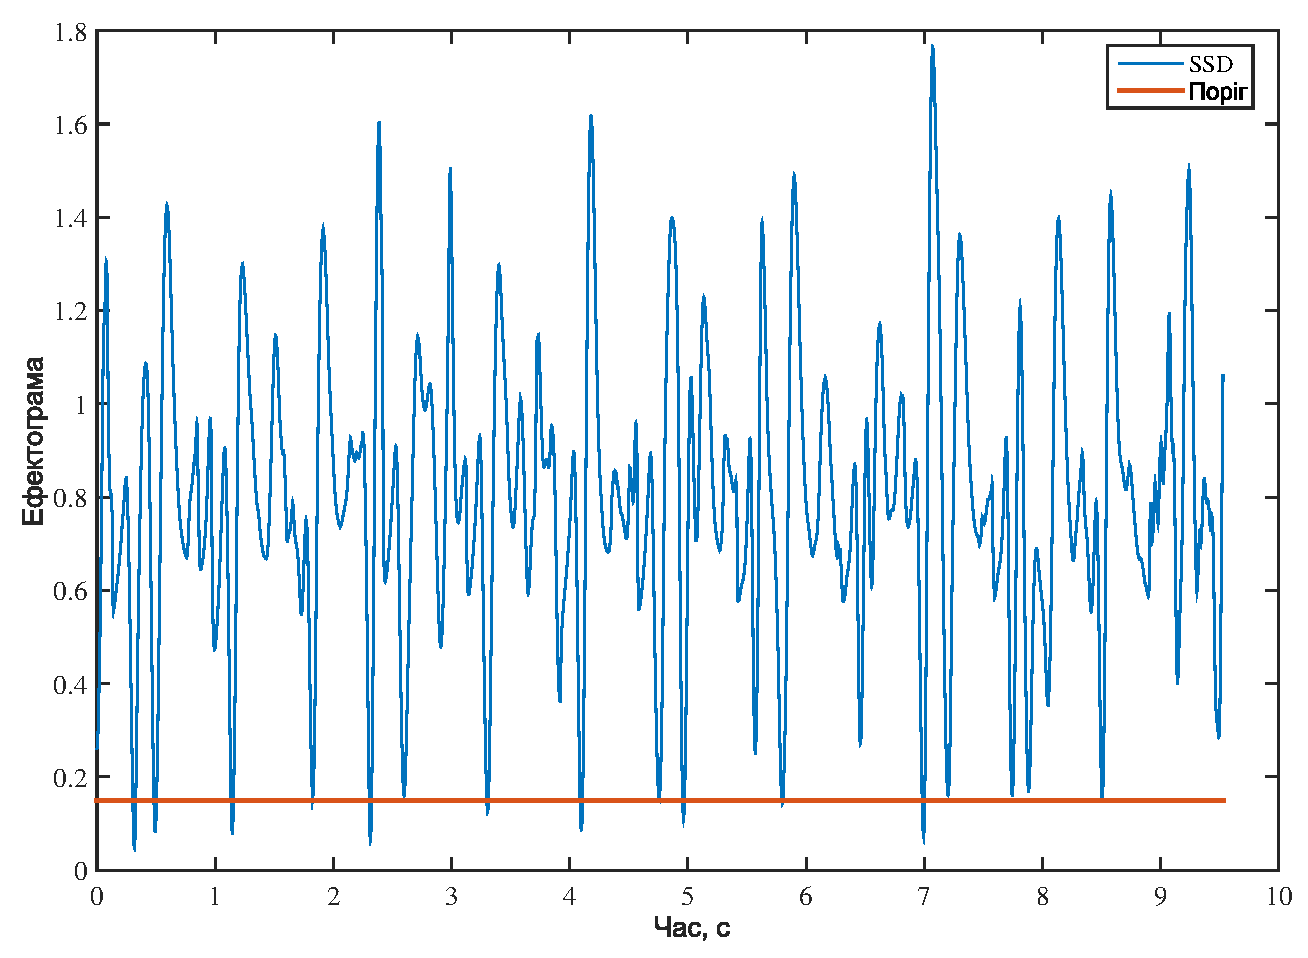
\includegraphics[height=0.28\textheight]{audio-energy-rect-min-ssd-han.eps}
            }
            % 3.24

            \subfloat[Kunchenko]{%
                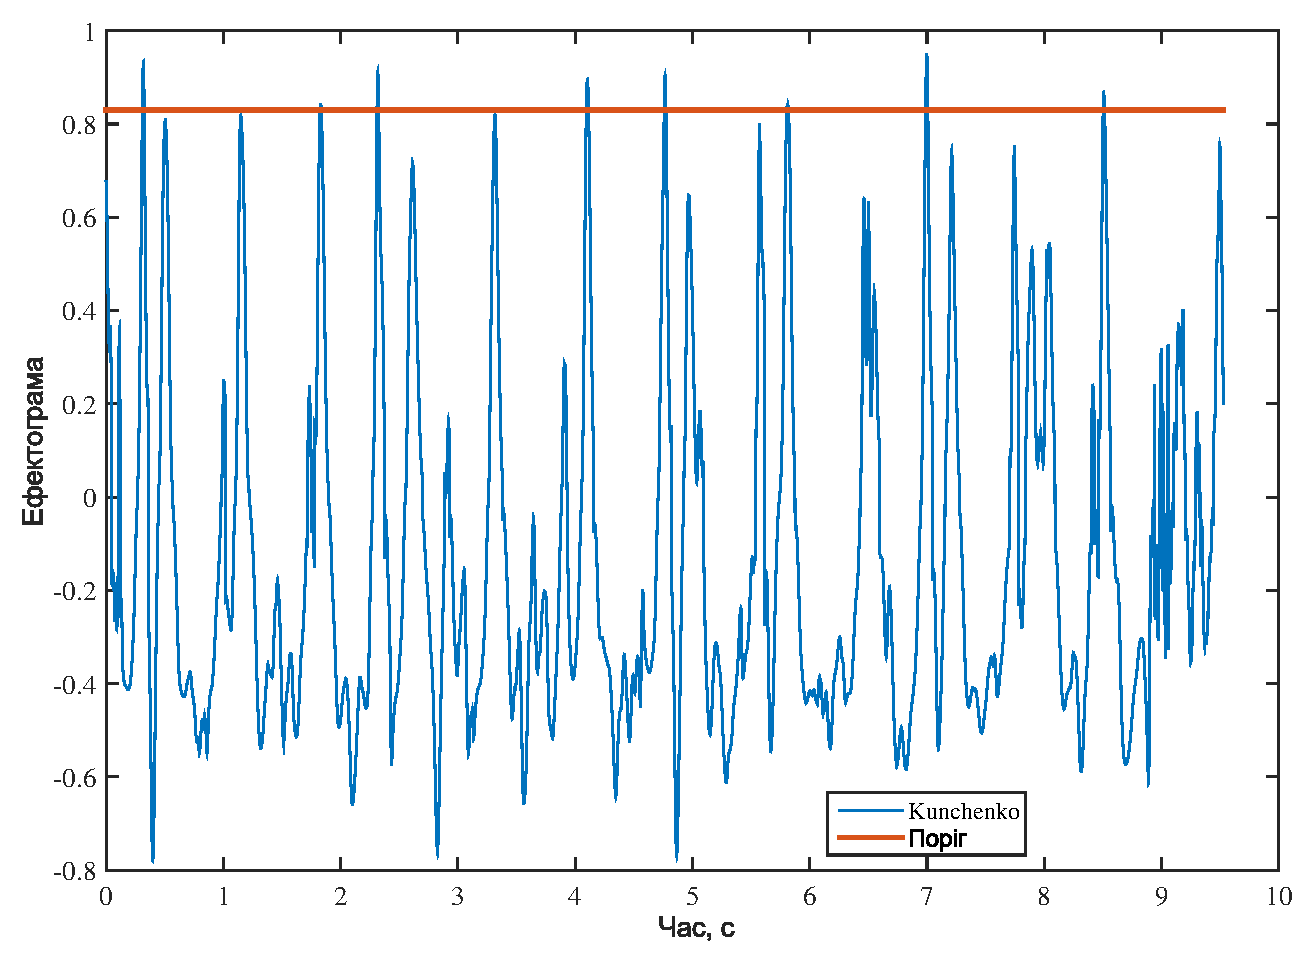
\includegraphics[height=0.28\textheight]{audio-energy-rect-min-kun-han.eps}
            }
            % 118.38

            \caption{Знайдений шаблон в енергії, наведеної на рисунку~\ref{fig:audio-energy-rect-min},
                використовуючи вікна Гана}
            \label{fig:matched-energy-rect-min-hann}
        \end{figure}

        \stepcounter{figurecount}
        \begin{figure}[h]
            \centering
            \subfloat[NCC]{%
                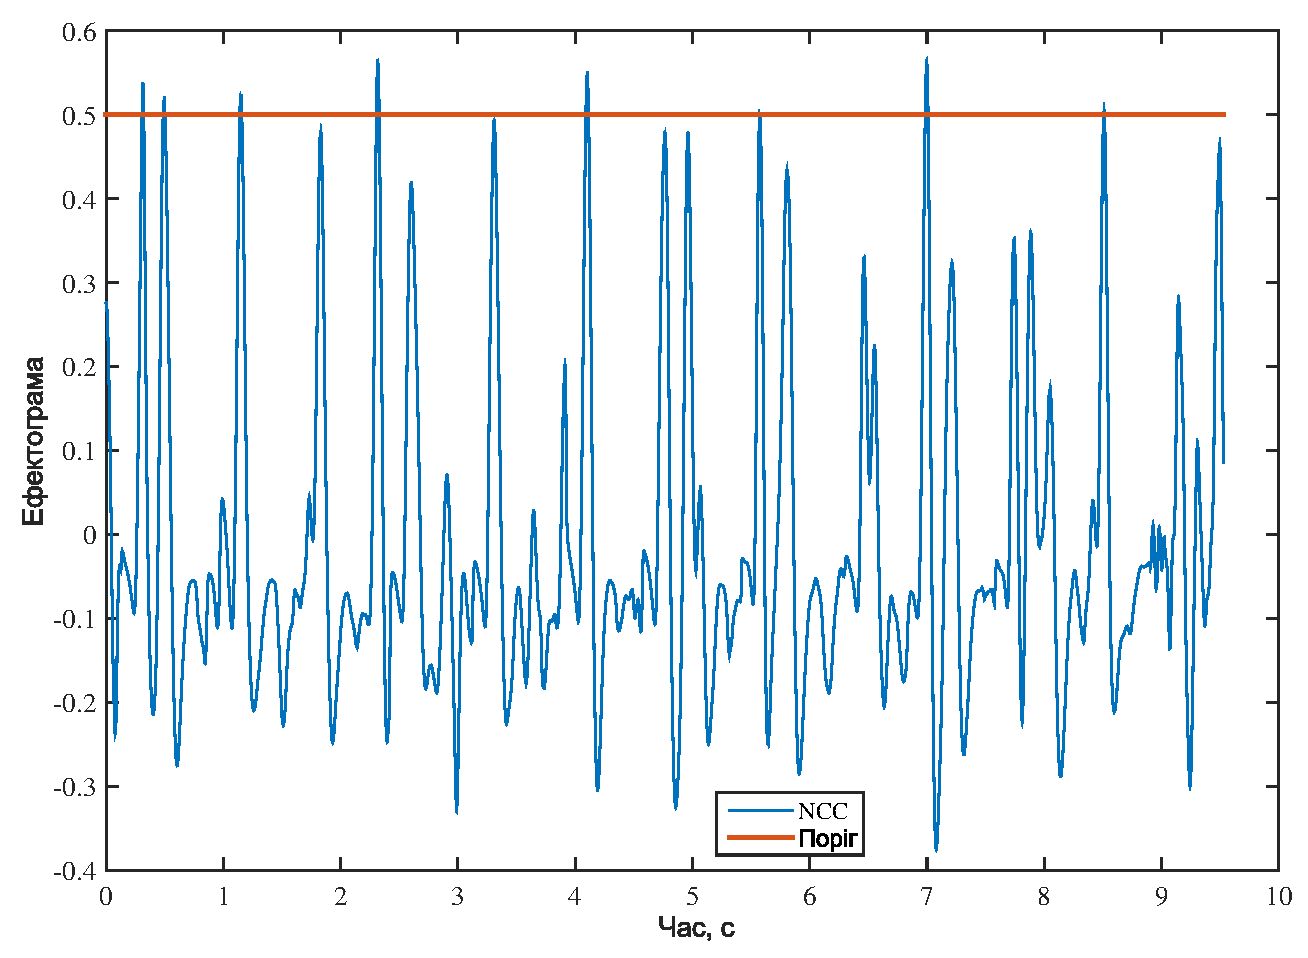
\includegraphics[height=0.28\textheight]{audio-energy-rect-min-ncc-hamming.eps}
            }
            % 3.17

            \subfloat[NSSD]{%
                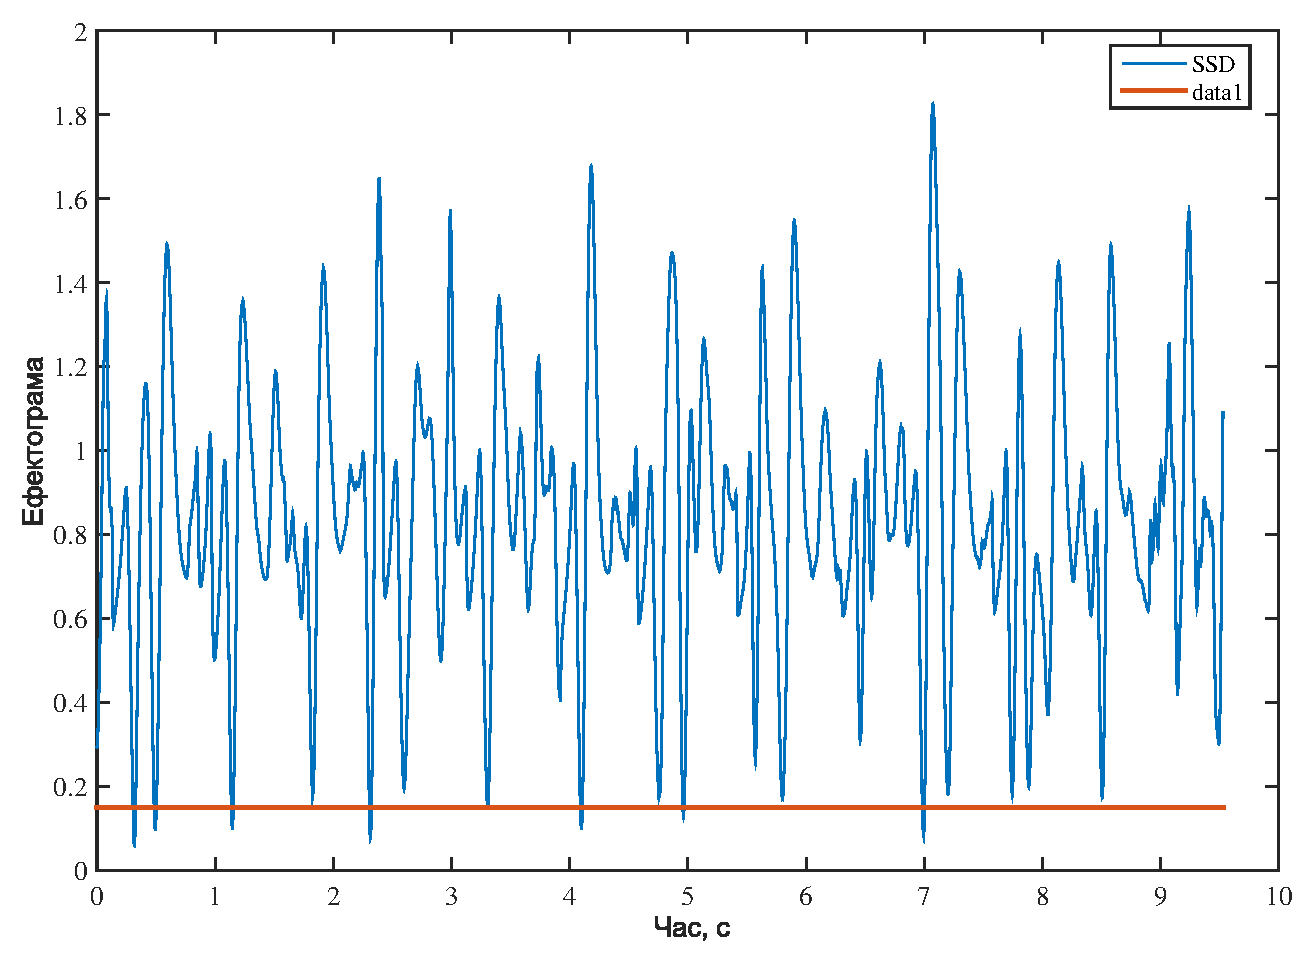
\includegraphics[height=0.28\textheight]{audio-energy-rect-min-ssd-hamming.eps}
            }
            % 3.35

            \subfloat[Kunchenko]{%
                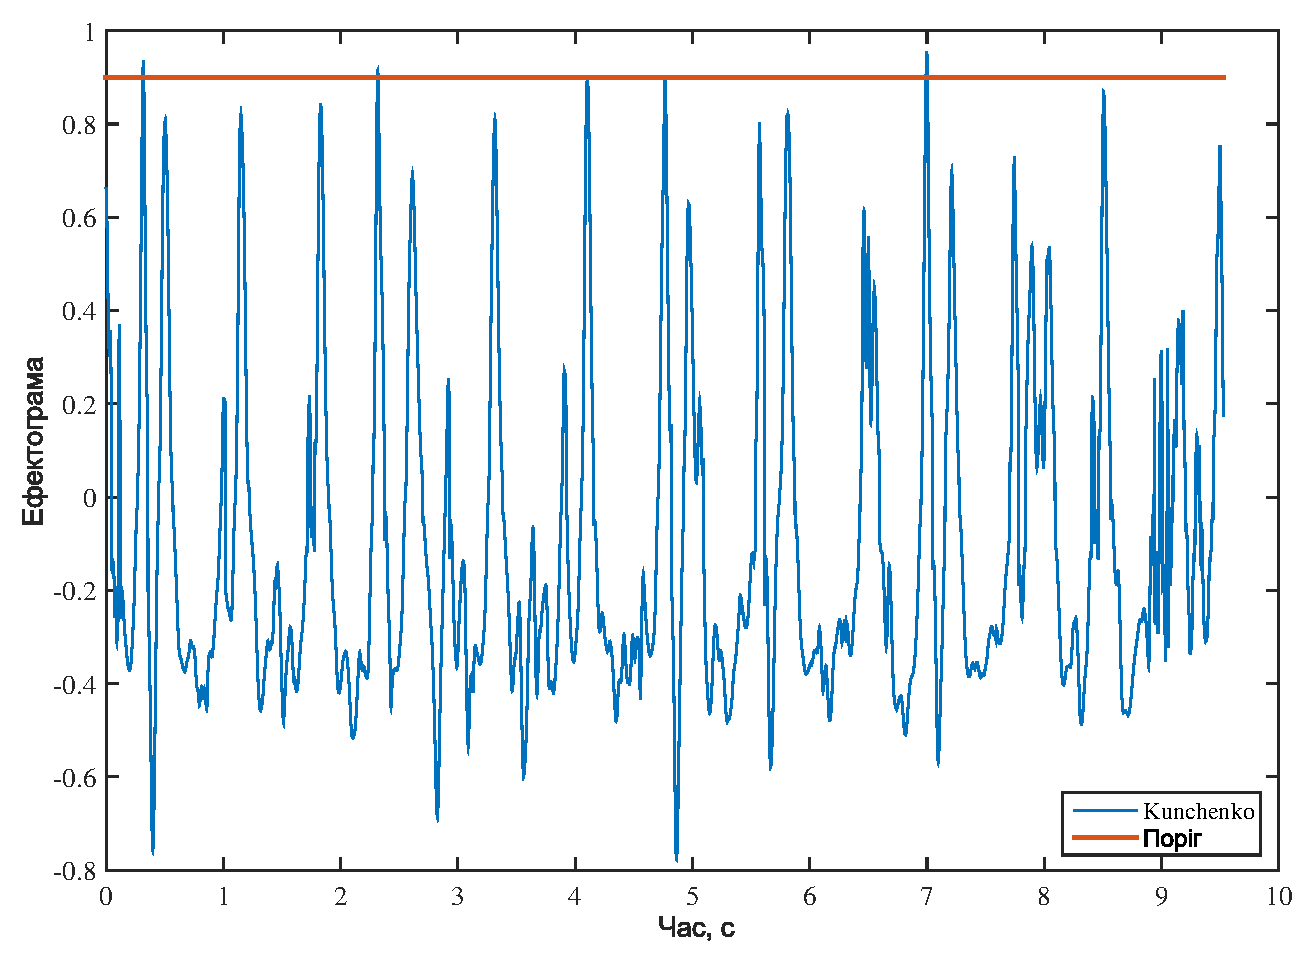
\includegraphics[height=0.28\textheight]{audio-energy-rect-min-kun-hamming.eps}
            }
            % 98.26

            \caption{Знайдений шаблон в енергії, наведеної на рисунку~\ref{fig:audio-energy-rect-min},
                використовуючи вікна Геммінга}
            \label{fig:matched-energy-rect-min-hamming}
        \end{figure}

        \clearpage

        Розглянемо поведінку розглянутих алгоритмів для пошуку шаблонів в коротко"=часовій енергії сигналу, що була
        отримана з використанням найпростішого й найшвидшого методу виділення вікон --- прямокутні вікна.
        Такі вікна бралися з кроком, що дорівнює половині вікна

        На рисунку~\ref{fig:audio-energy-rect-half} на сторінці~\pageref{fig:audio-energy-rect-half} наведений
        вигляд коротко"=часової енергії шаблону та сигналу, що були отримані вказаним способом.
        Як видно з цього рисунку, отримані коротко"=часові енергії мають значно менше значень, а тому мають менш
        деталізований вигляд.

        На рисунках~\ref{fig:matched-energy-rect-half-rect} та~\ref{fig:matched-energy-rect-half-hamming} на
        сторінках~\pageref{fig:matched-energy-rect-half-rect} та~\pageref{fig:matched-energy-rect-half-hamming}
        відповідно, зображено результати пошуку шаблону в аудіосигналі.

        З цих результатів видно, що використання великого інтервалу між вікнами дозволяє отримувати дуже схожі
        результати, що й при використанні менших проміжків, але значно швидше (адже сигнал та шаблон складається зі
        значно меншої кількості значень).
        Проте, так само, як і в попередньому випадку, результати пошуку шаблонів в коротко"=часовій енергії, що була
        отримана з використанням прямокутних вікон мають невисоку точність.

        \stepcounter{figurecount}
        \begin{figure}[h]
            \centering
            \subfloat[Сигнал]{%
                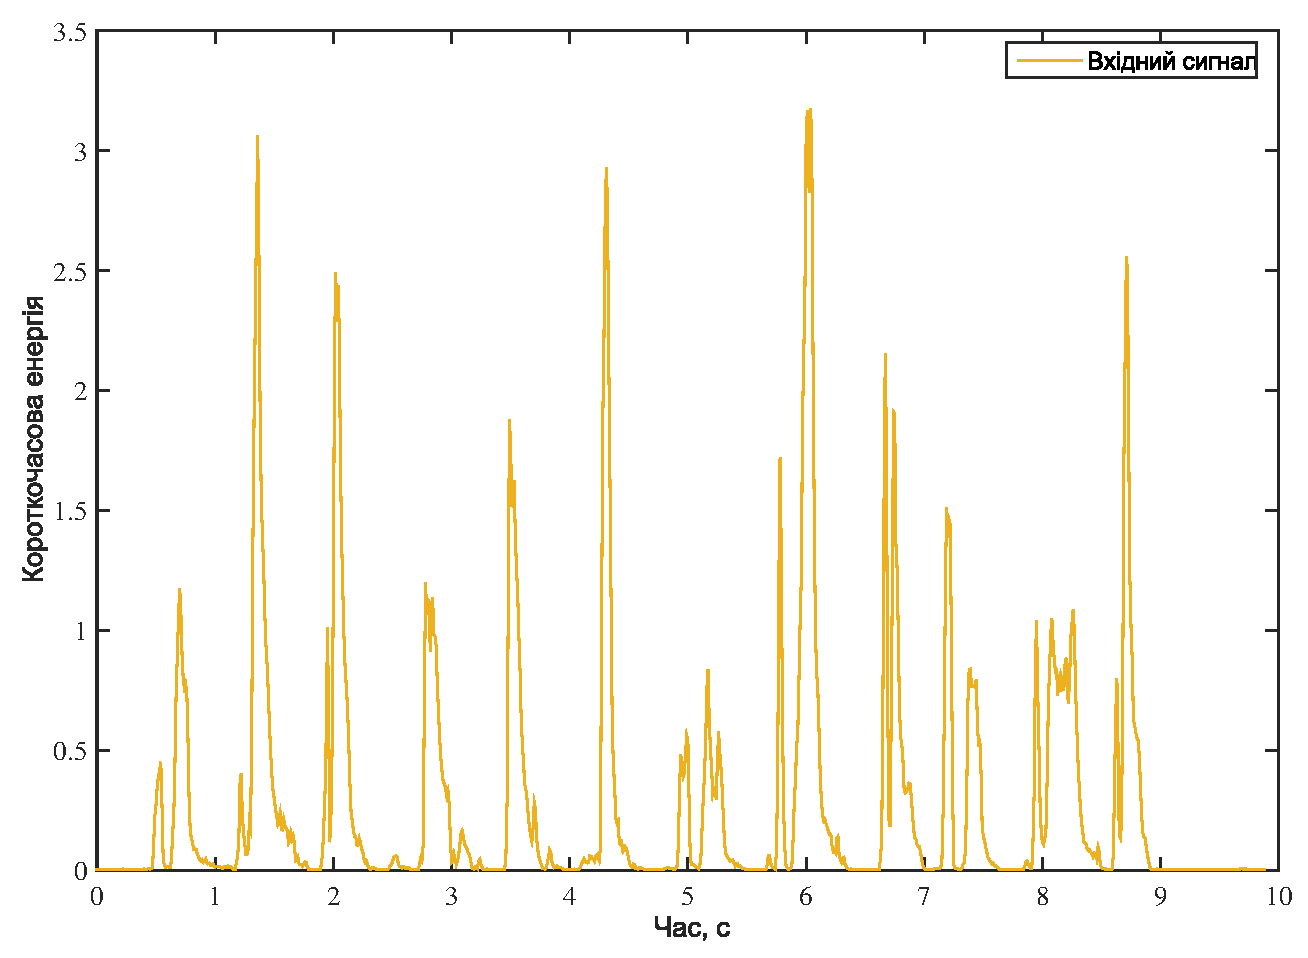
\includegraphics[width=0.8\textwidth]{audio_energy_rect_half.eps}
            }

            \subfloat[Зразок]{%
                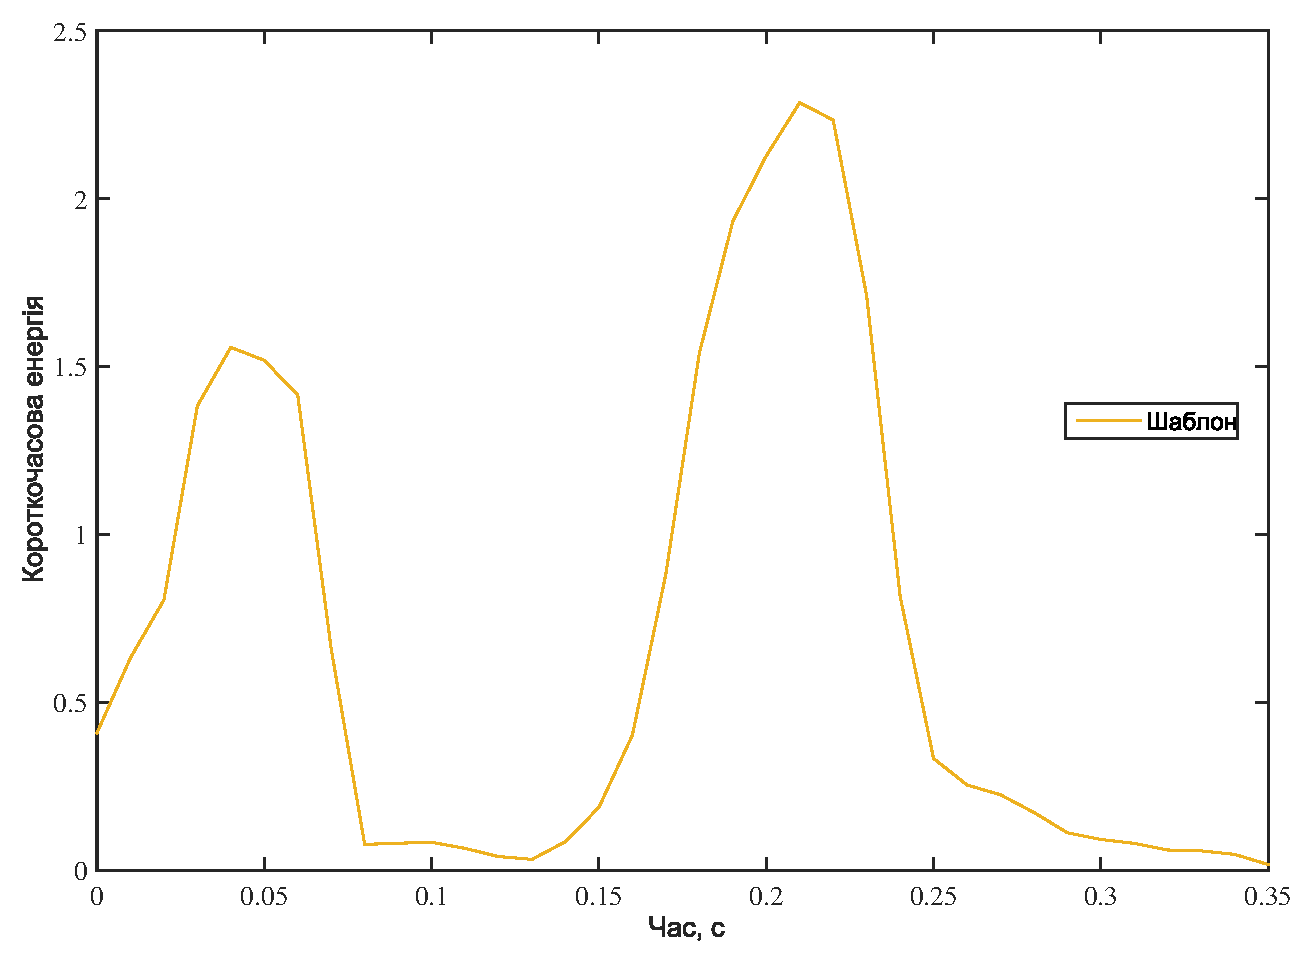
\includegraphics[width=0.8\textwidth]{audio_t_energy_rect_half.eps}
            }
            \caption{Короткочасна енергія запису мовлення й шаблону для пошуку використовуючи прямокутне вікно та крок
                середнього розміру}
            \label{fig:audio-energy-rect-half}
        \end{figure}

        \stepcounter{figurecount}
        \begin{figure}[h]
            \centering
            \subfloat[NCC]{%
                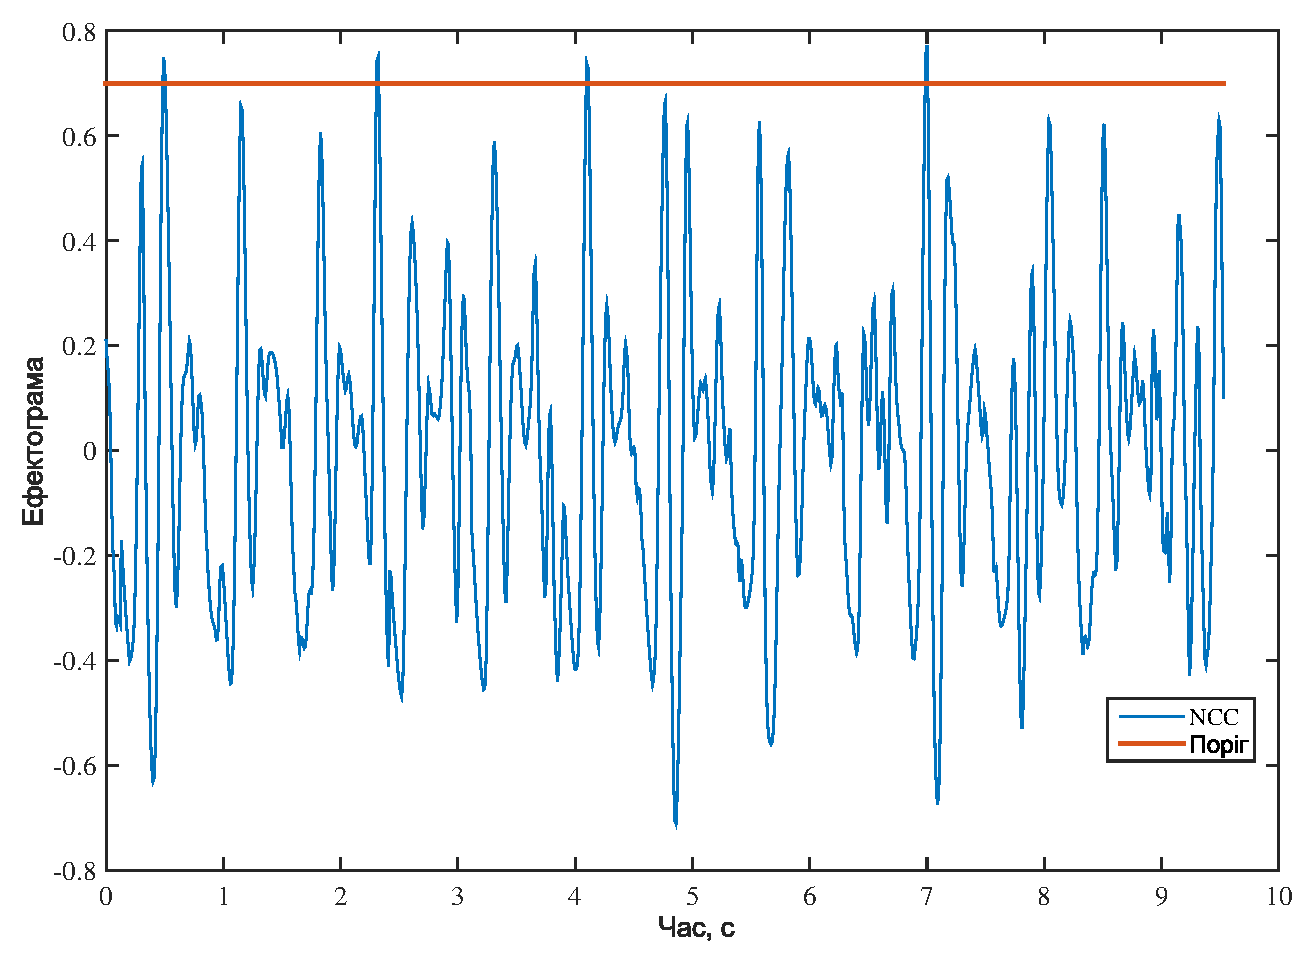
\includegraphics[height=0.28\textheight]{audio-energy-rect-half-ncc-rect.eps}
            }
            % 0

            \subfloat[NSSD]{%
                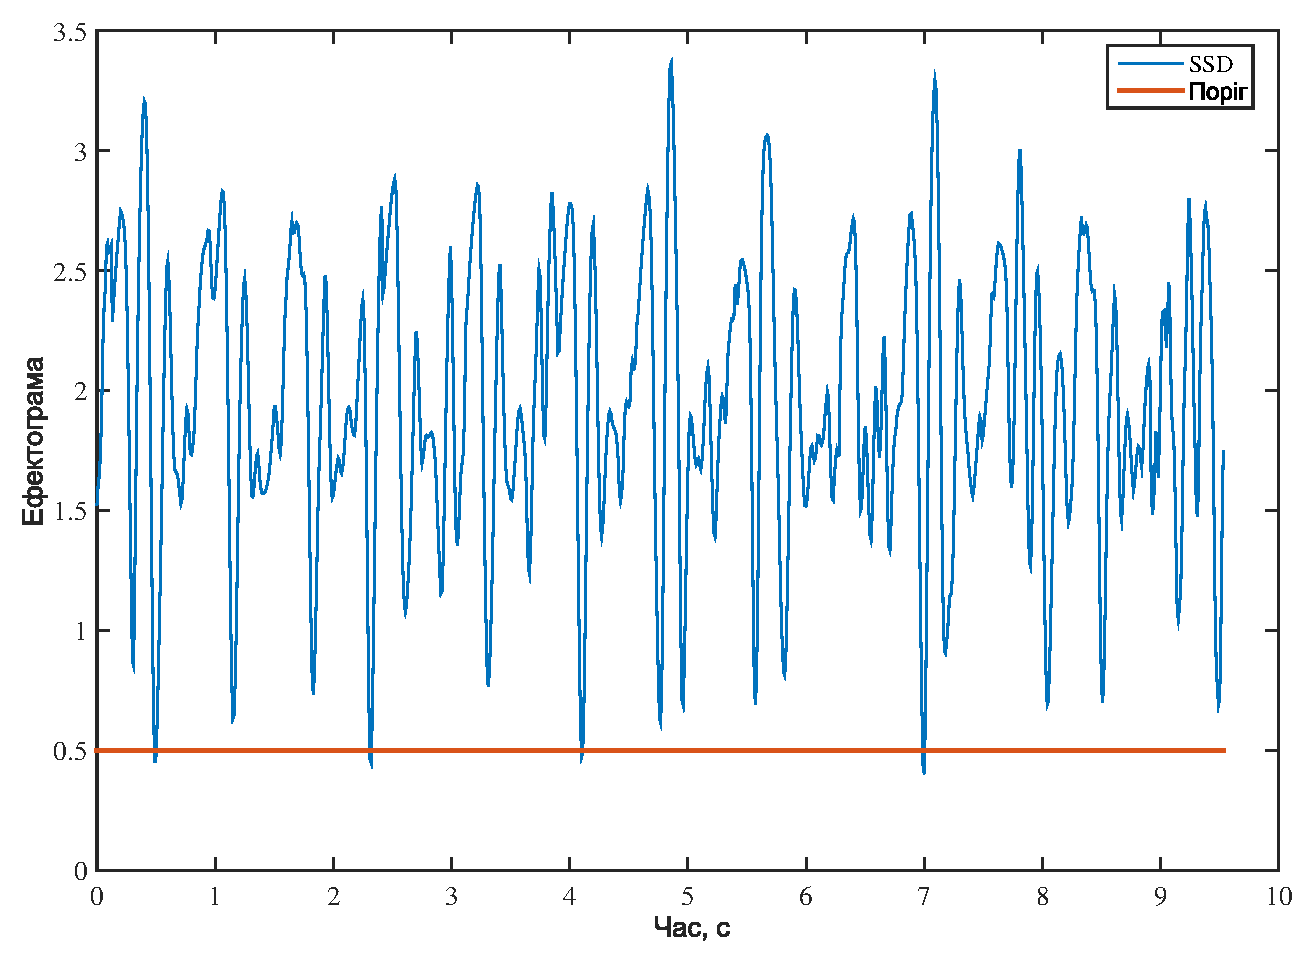
\includegraphics[height=0.28\textheight]{audio-energy-rect-half-ssd-rect.eps}
            }
            % 0

            \subfloat[Kunchenko]{%
                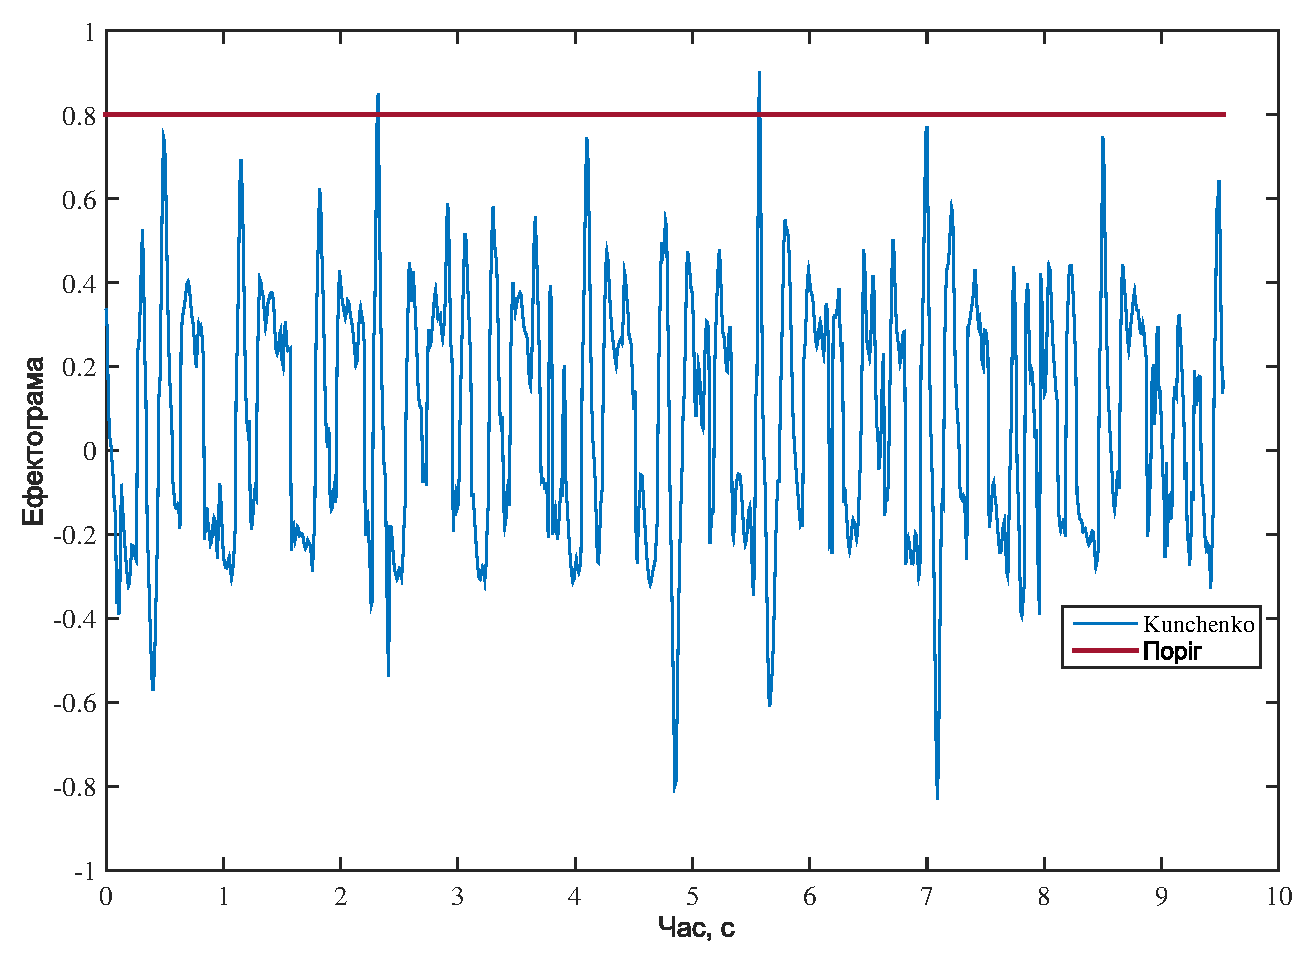
\includegraphics[height=0.28\textheight]{audio-energy-rect-half-kun-rect.eps}
            }
            % 0.8

            \caption{Знайдений шаблон в енергії, наведеної на рисунку~\ref{fig:audio-energy-rect-half}, використовуючи
                прямокутні вікна}
            \label{fig:matched-energy-rect-half-rect}
        \end{figure}

        \stepcounter{figurecount}
        \begin{figure}[h]
            \centering
            \subfloat[NCC]{%
                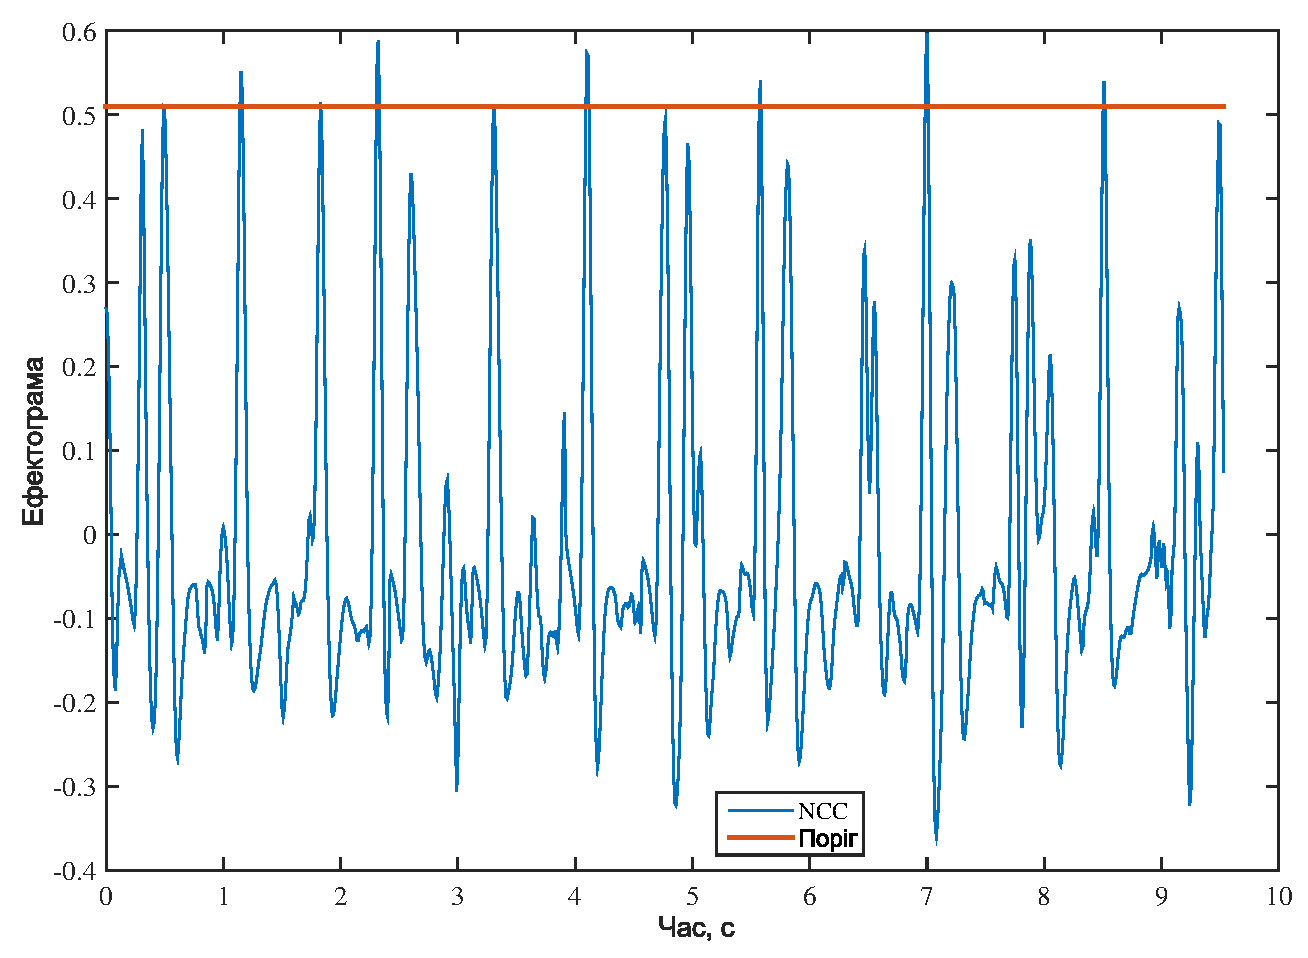
\includegraphics[height=0.28\textheight]{audio-energy-rect-half-ncc-hamming.eps}
            }
            % 0.01

            \subfloat[NSSD]{%
                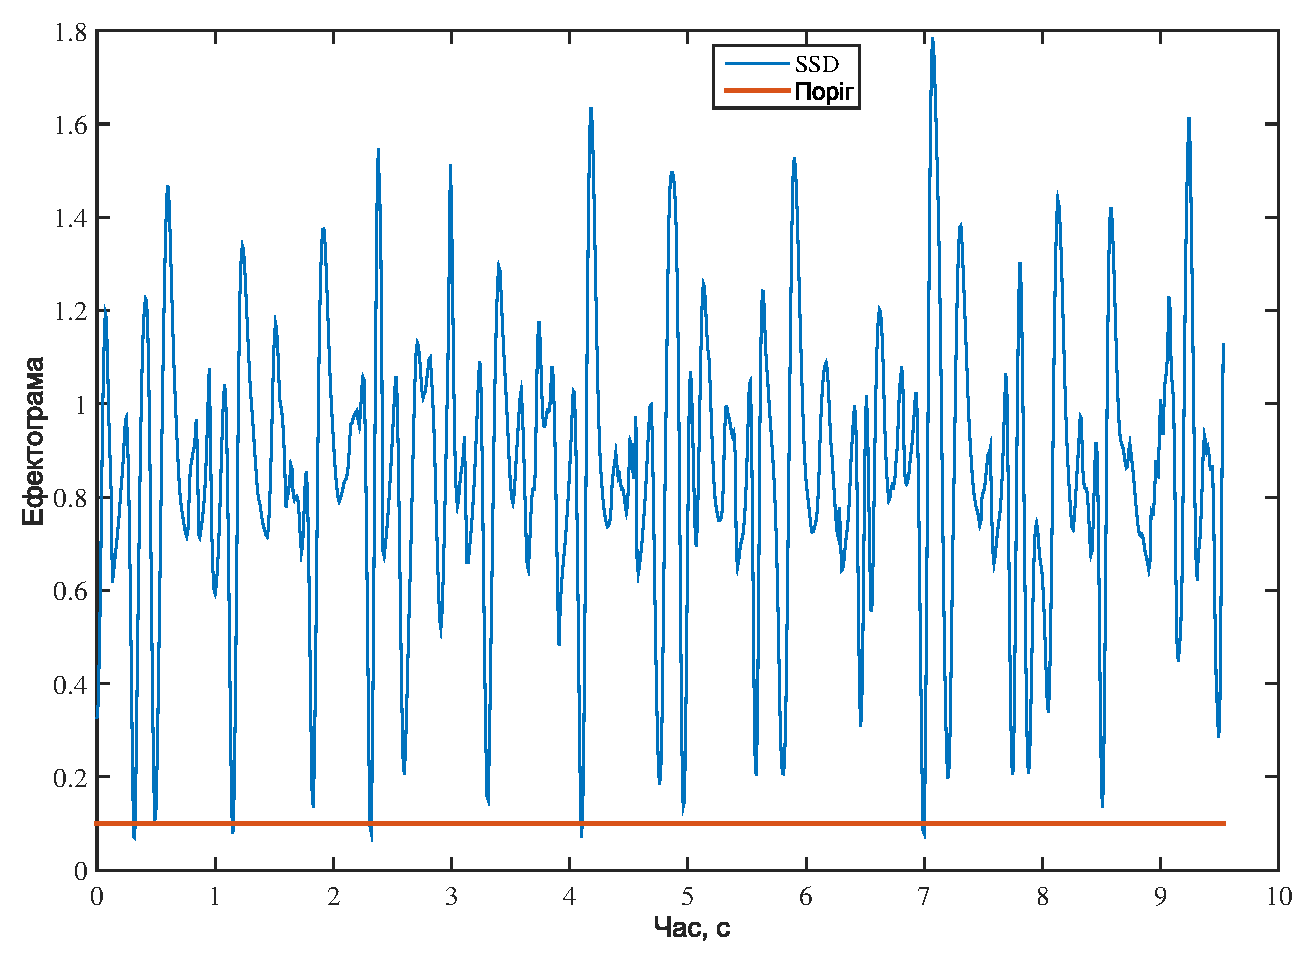
\includegraphics[height=0.28\textheight]{audio-energy-rect-half-ssd-hamming.eps}
            }
            % 0

            \subfloat[Kunchenko]{%
                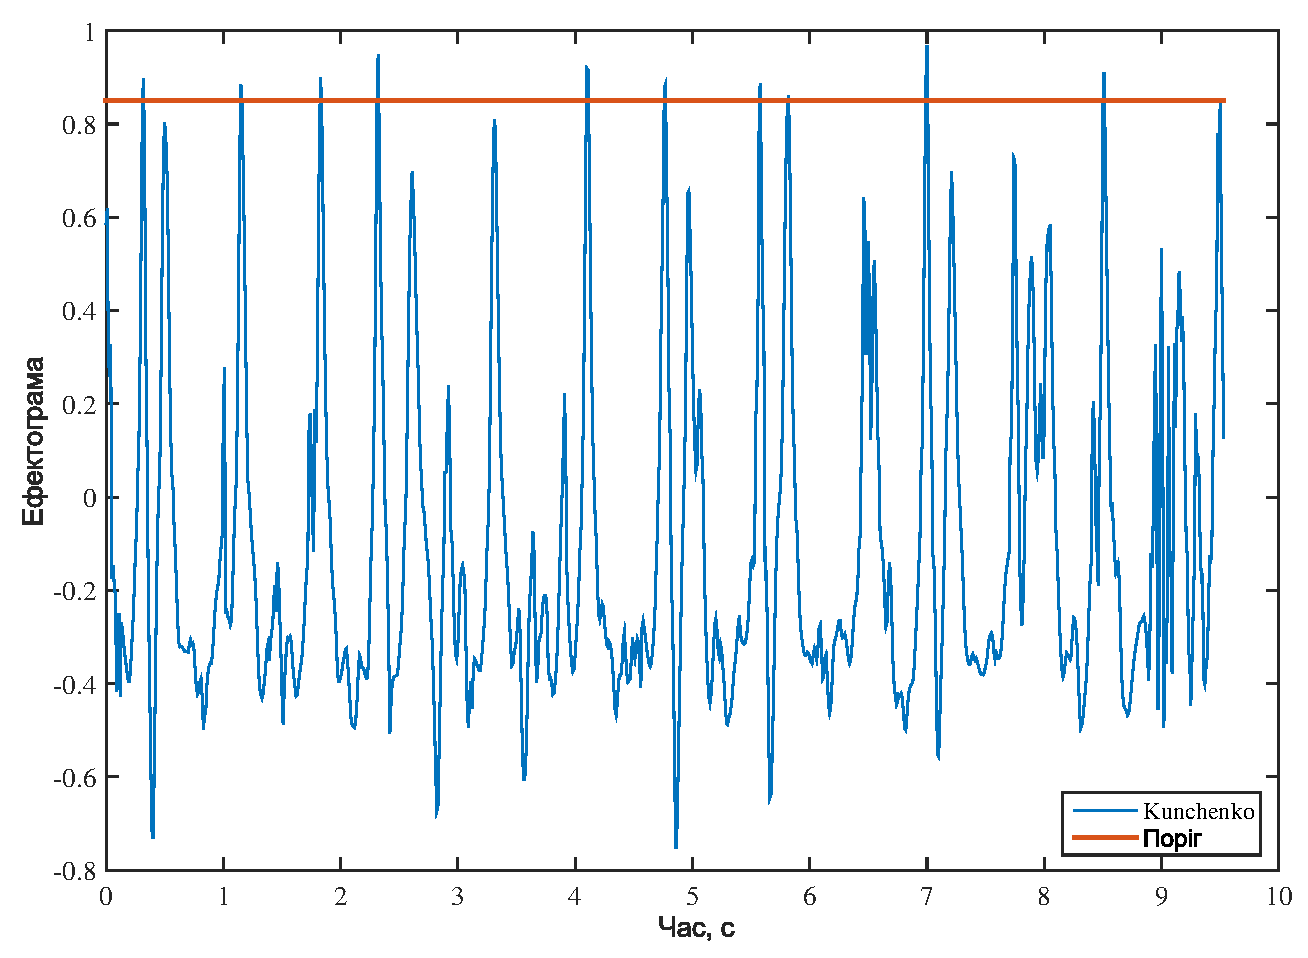
\includegraphics[height=0.28\textheight]{audio-energy-rect-half-kun-hamming.eps}
            }
            % 1.03

            \caption{Знайдений шаблон в енергії, наведеної на рисунку~\ref{fig:audio-energy-rect-half}, використовуючи
                вікна Геммінга}
            \label{fig:matched-energy-rect-half-hamming}
        \end{figure}

        \clearpage

        % HAN
        Розглянемо поведінку розглянутих алгоритмів для пошуку шаблонів в коротко"=часовій енергії сигналу, що була
        отримана з використанням віконної функції Гана.
        Такі вікна бралися з кроком, що дорівнює кроку дискретизації, тобто з мінімально"=можливим кроком.

        На рисунку~\ref{fig:audio-energy-han-min} на сторінці~\pageref{fig:audio-energy-han-min} наведений
        вигляд коротко"=часової енергії шаблону та сигналу, що були отримані вказаним способом.
        Як видно з цього рисунку, отримані коротко"=часові енергії мають більш гладку форму, ніж коротко"=часова
        енергія, що була отримана з використанням прямокутного вікна.

        На рисунках~\ref{fig:matched-energy-han-min-rect} та~\ref{fig:matched-energy-han-min-hamming} на
        сторінках~\pageref{fig:matched-energy-han-min-rect} та~\pageref{fig:matched-energy-han-min-hamming}
        відповідно, зображено результати пошуку шаблону в аудіосигналі.

        З цих результатів видно, що використання вікна Гана для обчислення коротко"=часової енергії призвело до того,
        що кількість хибних спрацювань алгоритмів значно зменшилась, але все рівно алгоритми мають невелику точність.

        \stepcounter{figurecount}
        \begin{figure}[h]
            \centering
            \subfloat[Сигнал]{%
                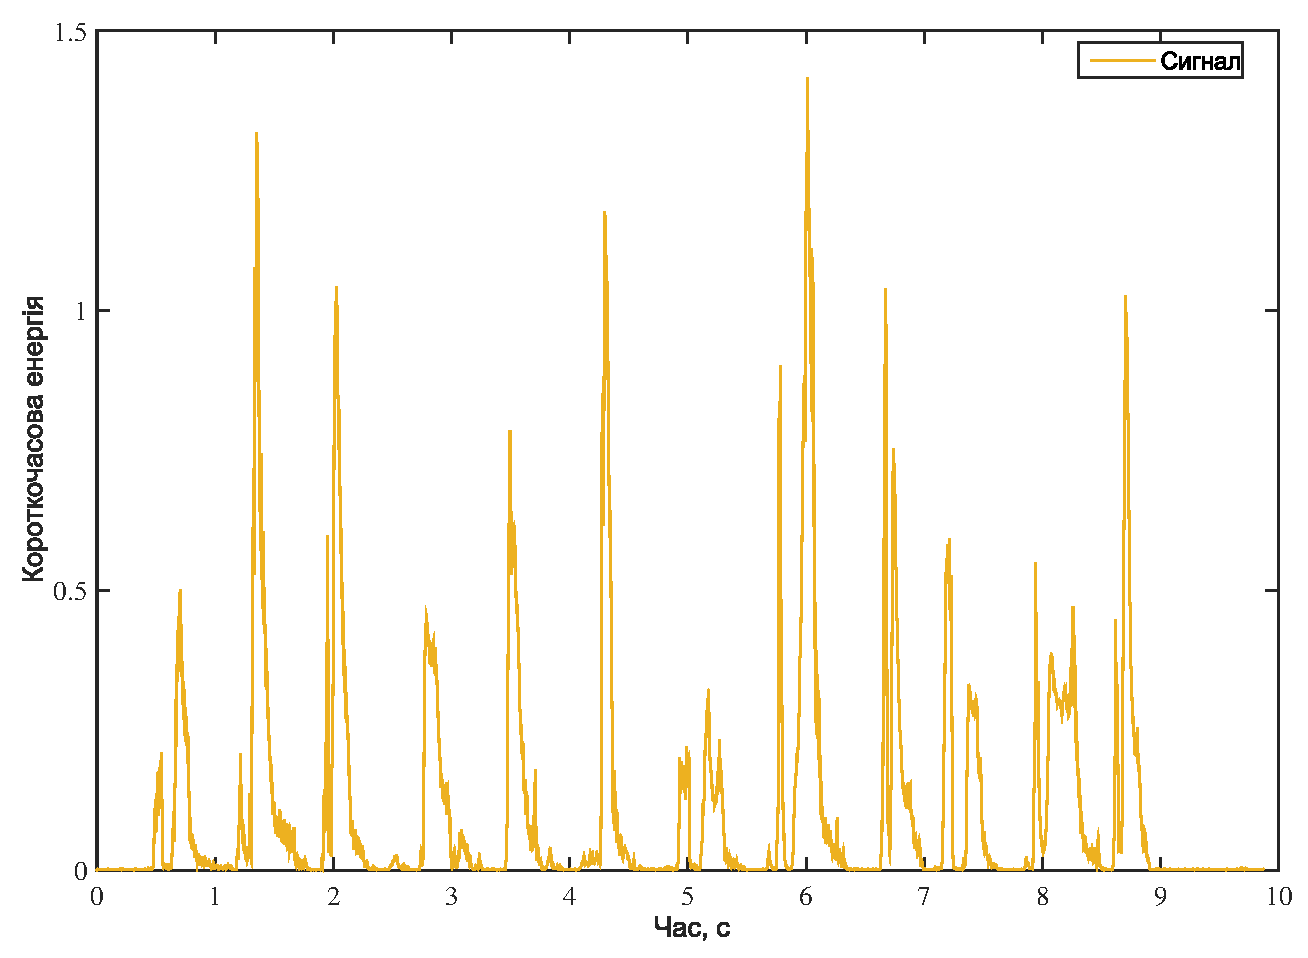
\includegraphics[width=0.8\textwidth]{audio_energy_han_min.eps}
            }

            \subfloat[Зразок]{%
                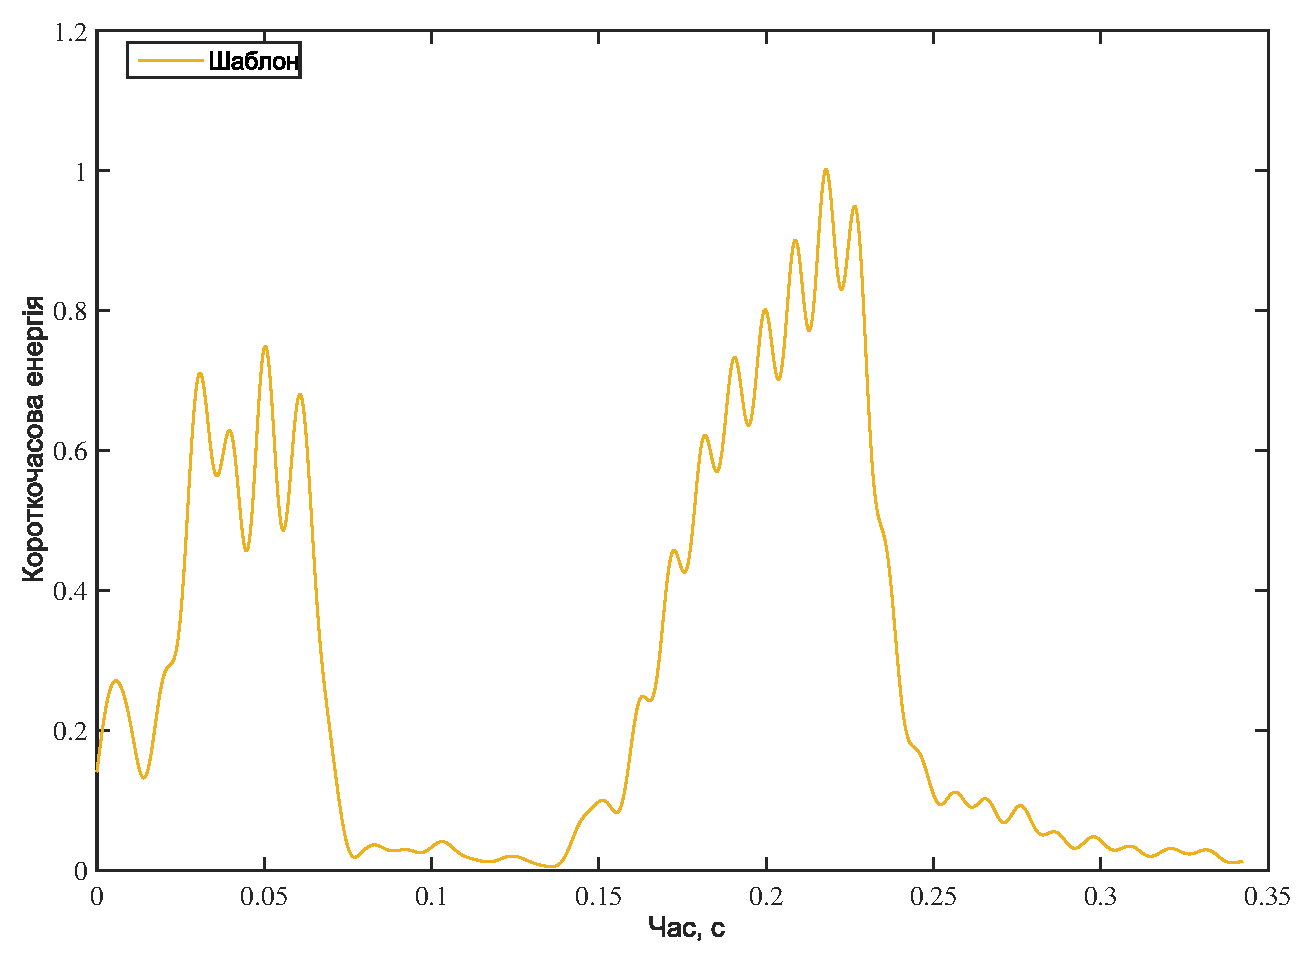
\includegraphics[width=0.8\textwidth]{audio_t_energy_han_min.eps}
            }
            \caption{Короткочасна енергія запису мовлення й шаблону для пошуку використовуючи вікно Гана та крок
                мінімального розміру}
            \label{fig:audio-energy-han-min}
        \end{figure}

        \stepcounter{figurecount}
        \begin{figure}[h]
            \centering
            \subfloat[NCC]{%
                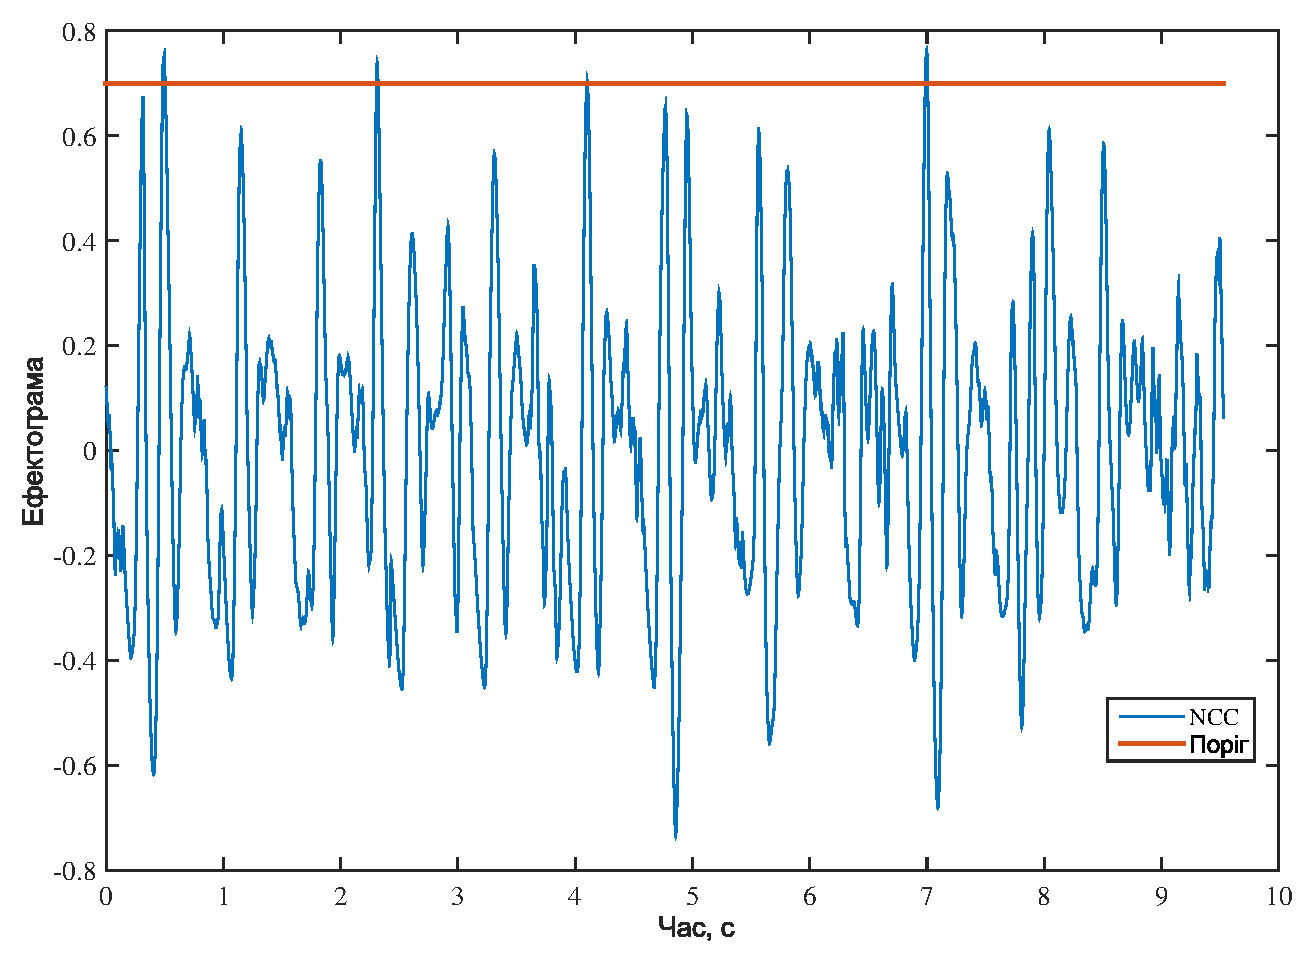
\includegraphics[height=0.28\textheight]{audio-energy-han-min-ncc-rect.eps}
            }
            % 2.52

            \subfloat[NSSD]{%
                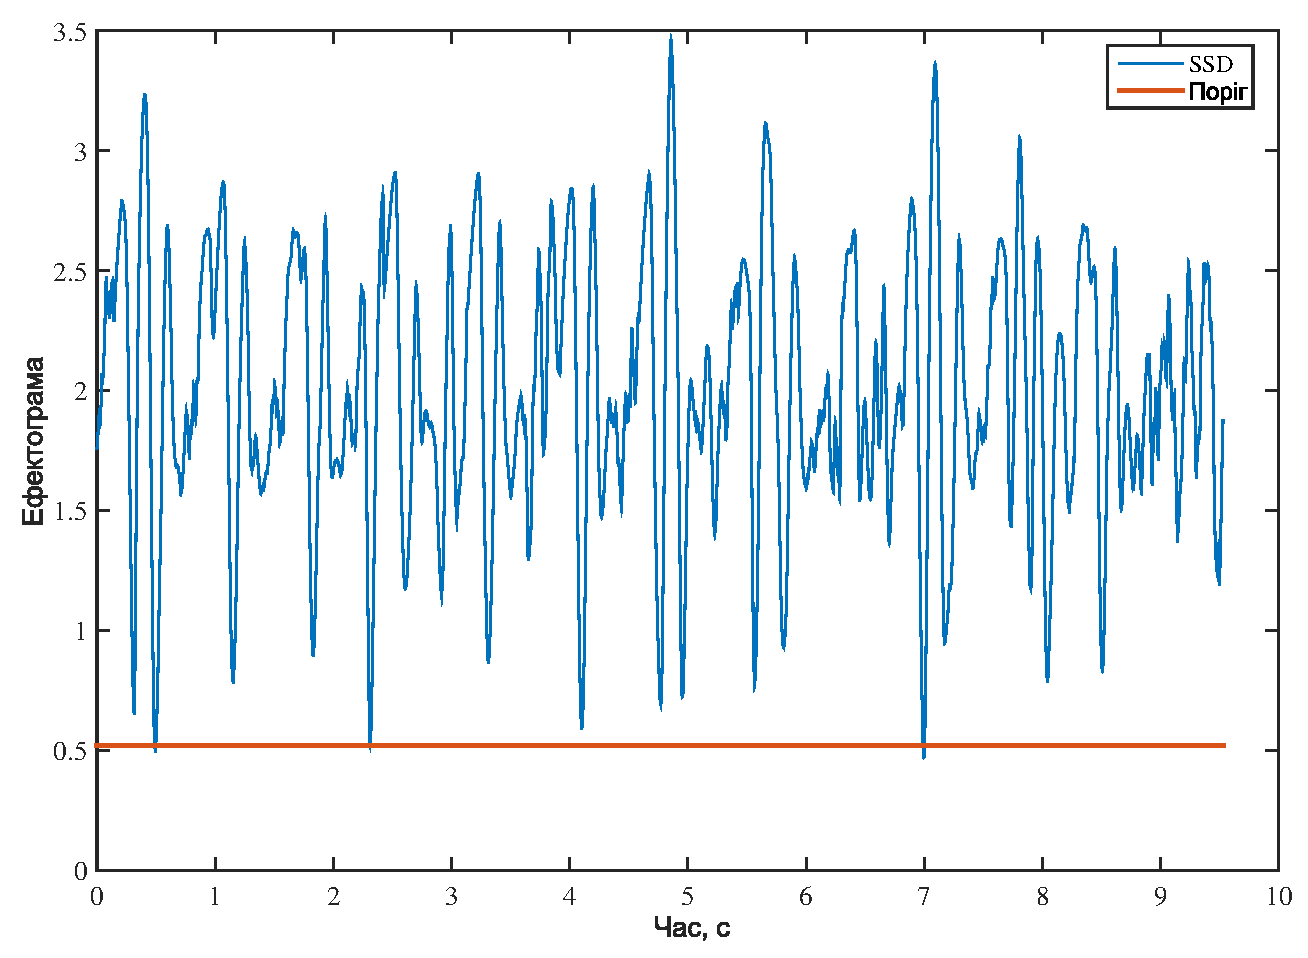
\includegraphics[height=0.28\textheight]{audio-energy-han-min-ssd-rect.eps}
            }
            % 2.70

            \subfloat[Kunchenko]{%
                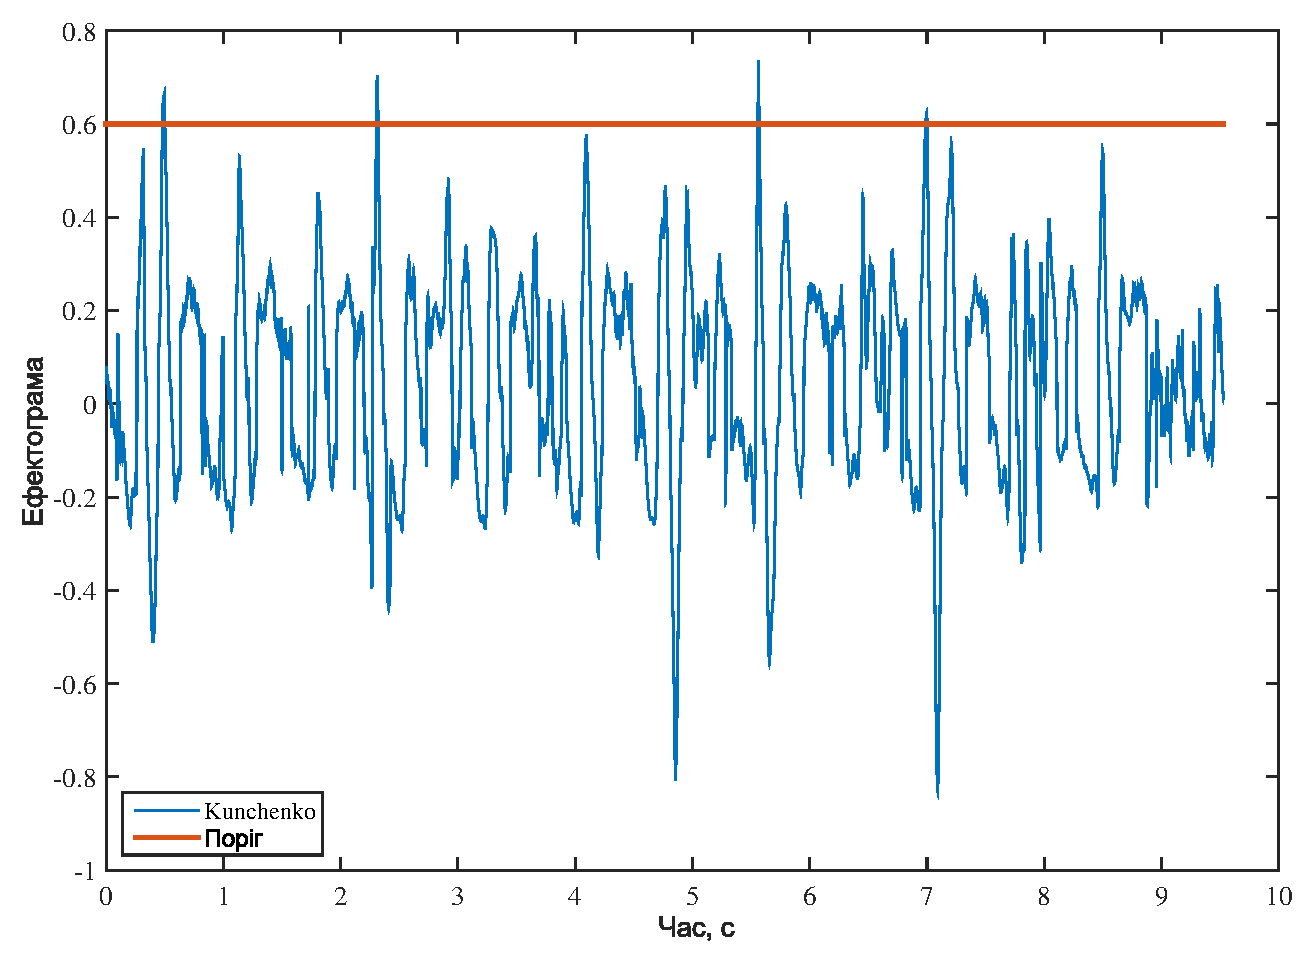
\includegraphics[height=0.28\textheight]{audio-energy-han-min-kun-rect.eps}
            }
            % 0.8
            \caption{Знайдений шаблон в енергії, наведеної на рисунку~\ref{fig:audio-energy-han-min}, використовуючи
                прямокутні вікна}
            \label{fig:matched-energy-han-min-rect}
        \end{figure}

        \stepcounter{figurecount}
        \begin{figure}[h]
            \centering
            \subfloat[NCC]{%
                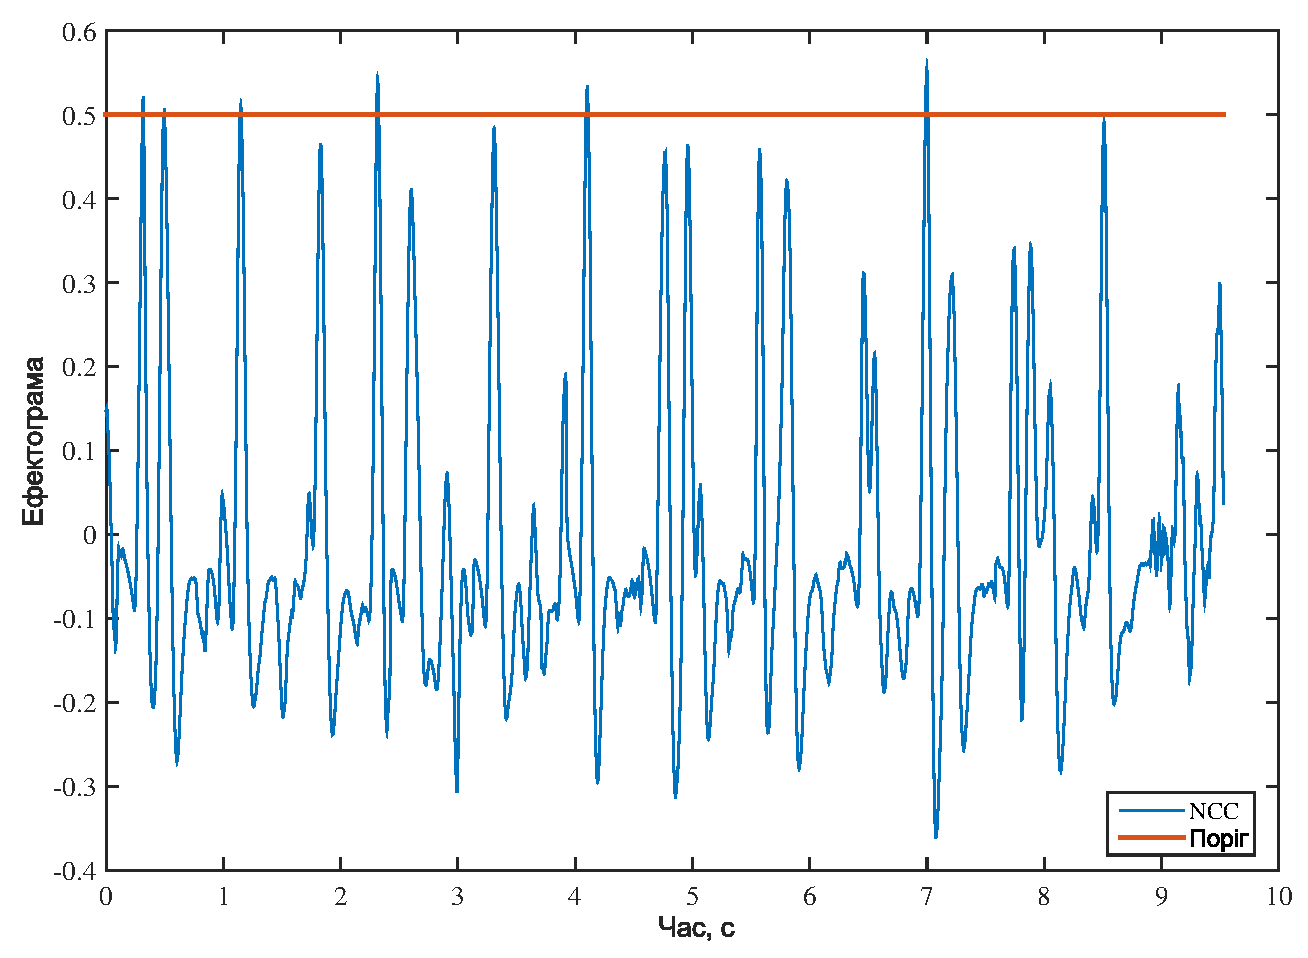
\includegraphics[height=0.28\textheight]{audio-energy-han-min-ncc-hamming.eps}
            }
            % 3.30

            \subfloat[NSSD]{%
                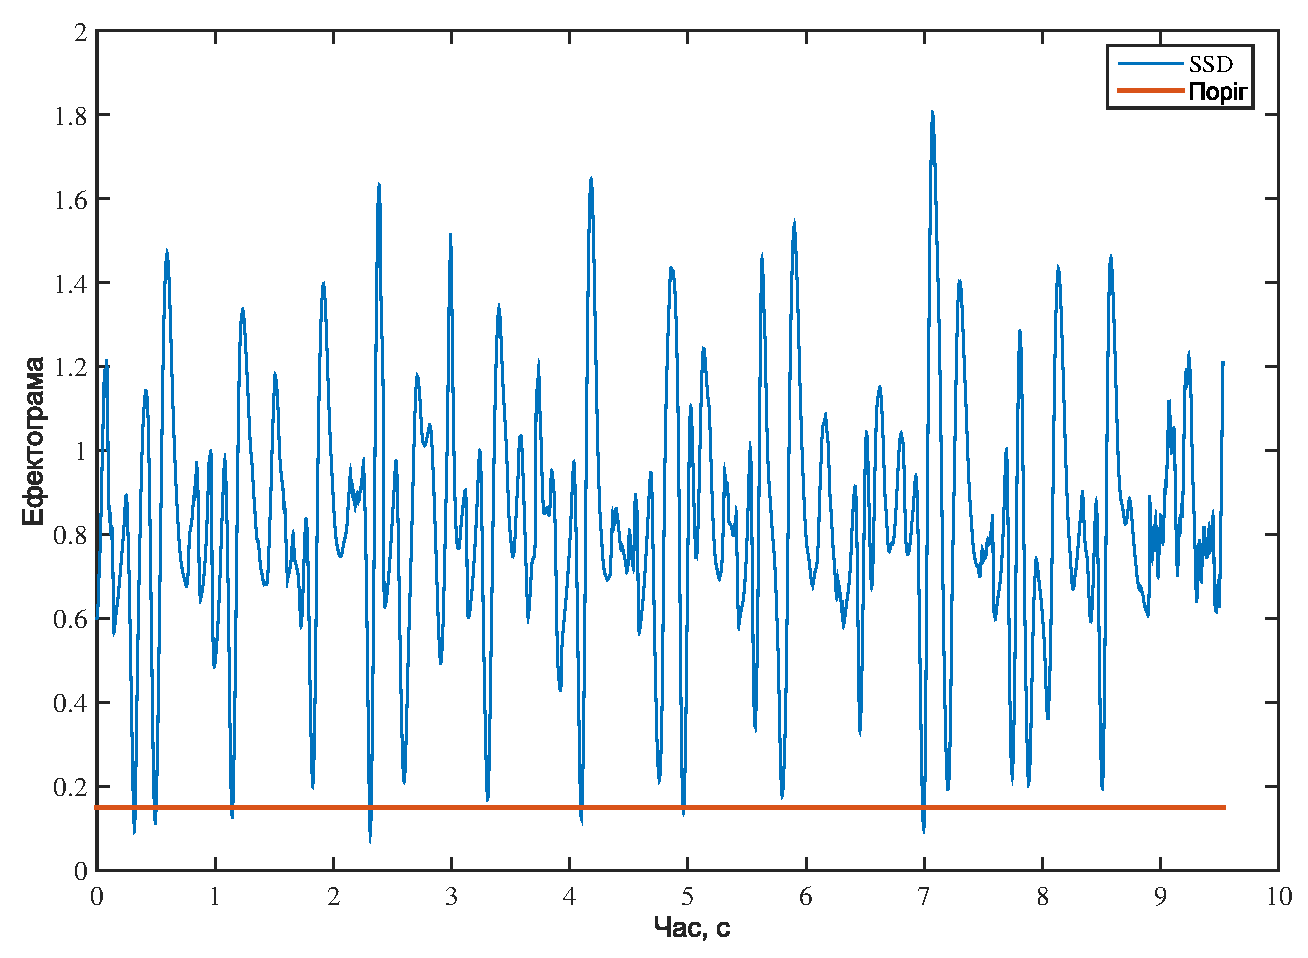
\includegraphics[height=0.28\textheight]{audio-energy-han-min-ssd-hamming.eps}
            }
            % 3.47

            \subfloat[Kunchenko]{%
                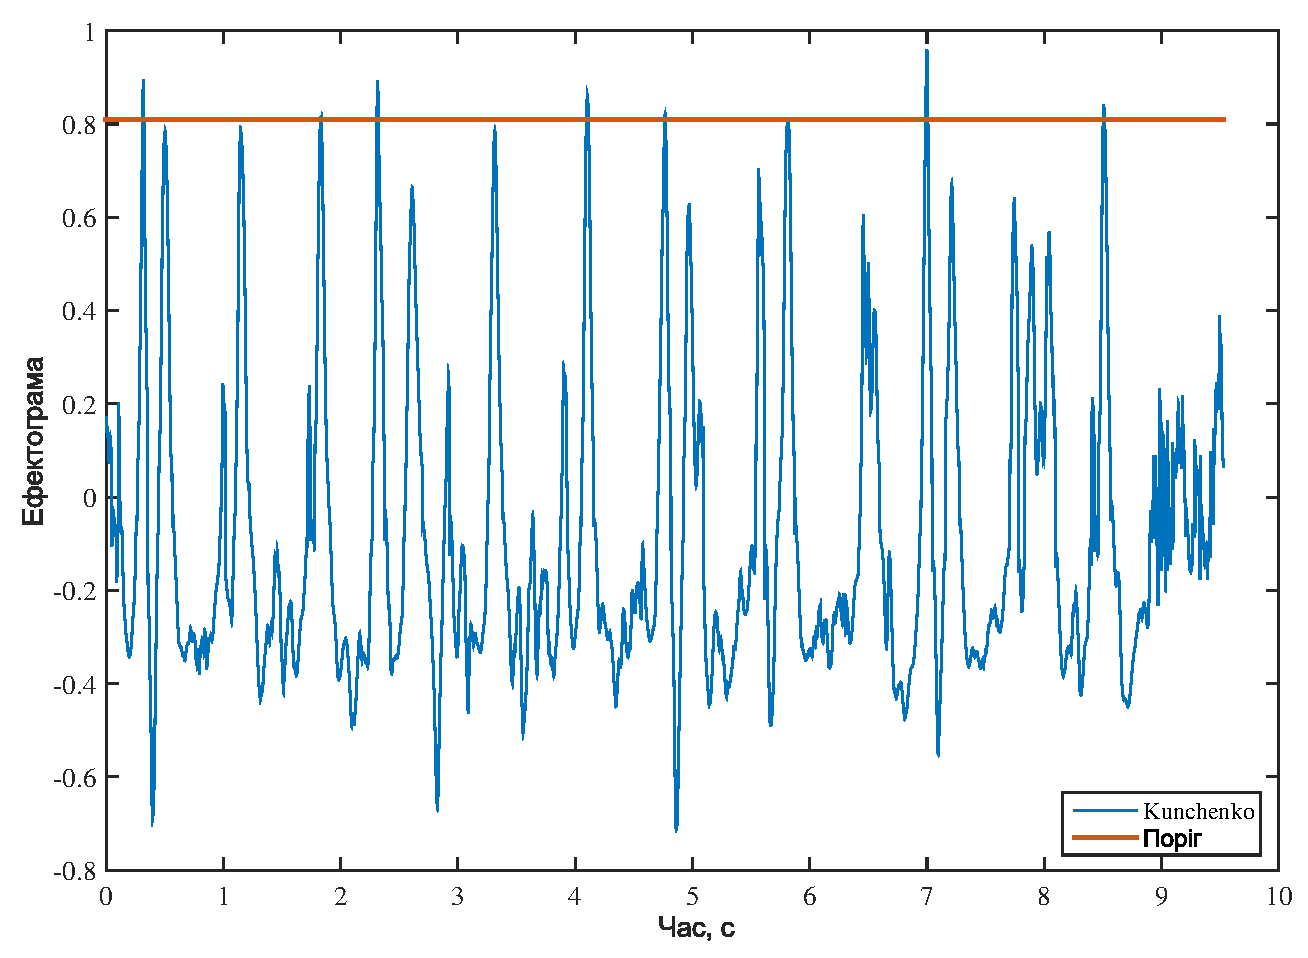
\includegraphics[height=0.28\textheight]{audio-energy-han-min-kun-hamming.eps}
            }
            % 138.36

            \caption{Знайдений шаблон в енергії, наведеної на рисунку~\ref{fig:audio-energy-han-min}, використовуючи
                вікна Геммінга}
            \label{fig:matched-energy-han-min-hamming}
        \end{figure}

        \clearpage

        % HAMMING
        Розглянемо поведінку розглянутих алгоритмів для пошуку шаблонів в коротко"=часовій енергії сигналу, що була
        отримана з використанням віконної функції Геммінга.
        Такі вікна бралися з кроком, що дорівнює кроку дискретизації, тобто з мінімально"=можливим кроком.

        На рисунку~\ref{fig:audio-energy-hamming-min} на сторінці~\pageref{fig:audio-energy-han-min} наведений
        вигляд коротко"=часової енергії шаблону та сигналу, що були отримані вказаним способом.
        По відношенню до коротко"=часової енергії, що була сгенерована з використанням вікна Гана, отримана енергія
        має менш різкі перепади на графіку.

        На рисунках~\ref{fig:matched-energy-hamming-min-rect} та~\ref{fig:matched-energy-han-min-hamming} на
        сторінках~\pageref{fig:matched-energy-hamming-min-rect} та~\pageref{fig:matched-energy-han-min-hamming}
        відповідно, зображено результати пошуку шаблону в аудіосигналі.

        З наведених графіків ефектограм видно, що для коротко"=часової енергії, що була згенерована саме таким чином,
        метод поліномів Кунченка знайшов усі входження шаблону до сигналу.
        Також необхідно зазначити той факт, що використання в методі ковзного вікна вікон, відмінних від прямокутного,
        на відміну від попередніх ситуацій, не призводило до зменшення амплітуди ефектограми для хибних спрацювань.

        \stepcounter{figurecount}
        \begin{figure}[h]
            \centering
            \subfloat[Сигнал]{%
                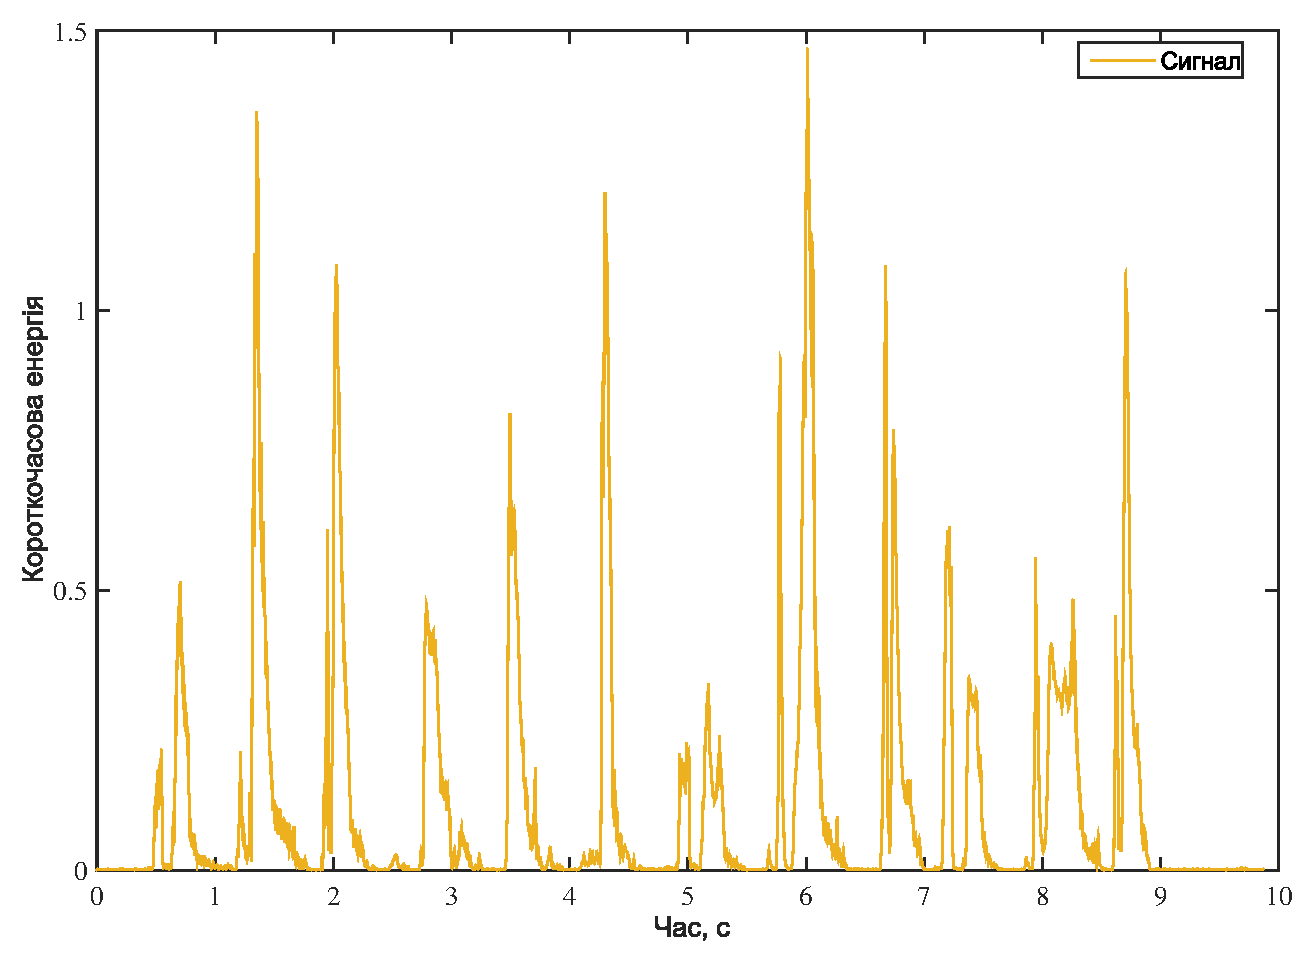
\includegraphics[width=0.8\textwidth]{audio_energy_hamming_min.eps}
            }

            \subfloat[Зразок]{%
                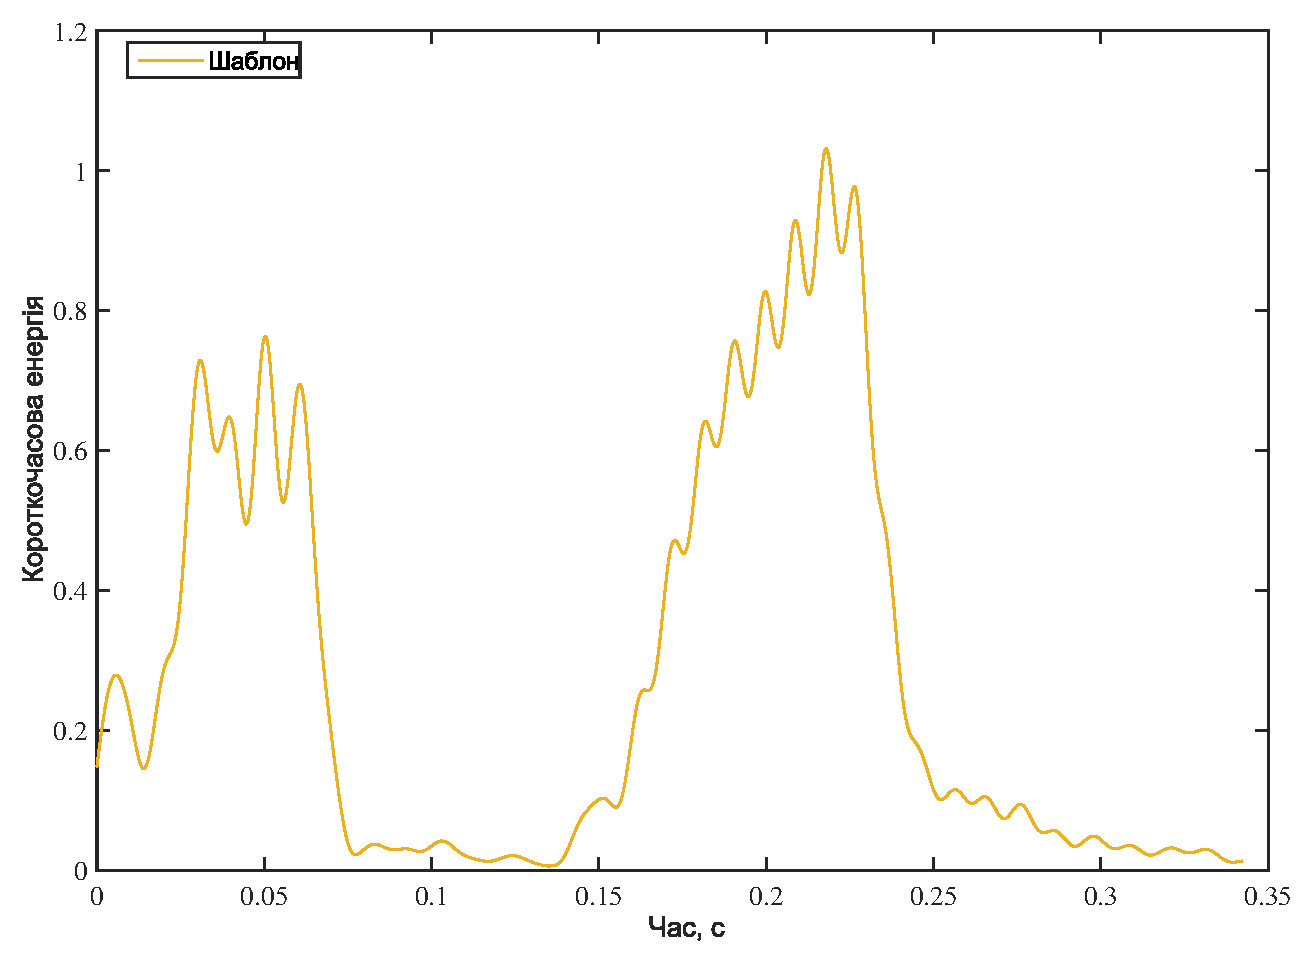
\includegraphics[width=0.8\textwidth]{audio_t_energy_hamming_min.eps}
            }
            \caption{Короткочасна енергія запису мовлення й шаблону для пошуку використовуючи вікно Геммінга та крок
                мінімального розміру}
            \label{fig:audio-energy-hamming-min}
        \end{figure}

        \stepcounter{figurecount}
        \begin{figure}[h]
            \centering
            \subfloat[NCC]{%
                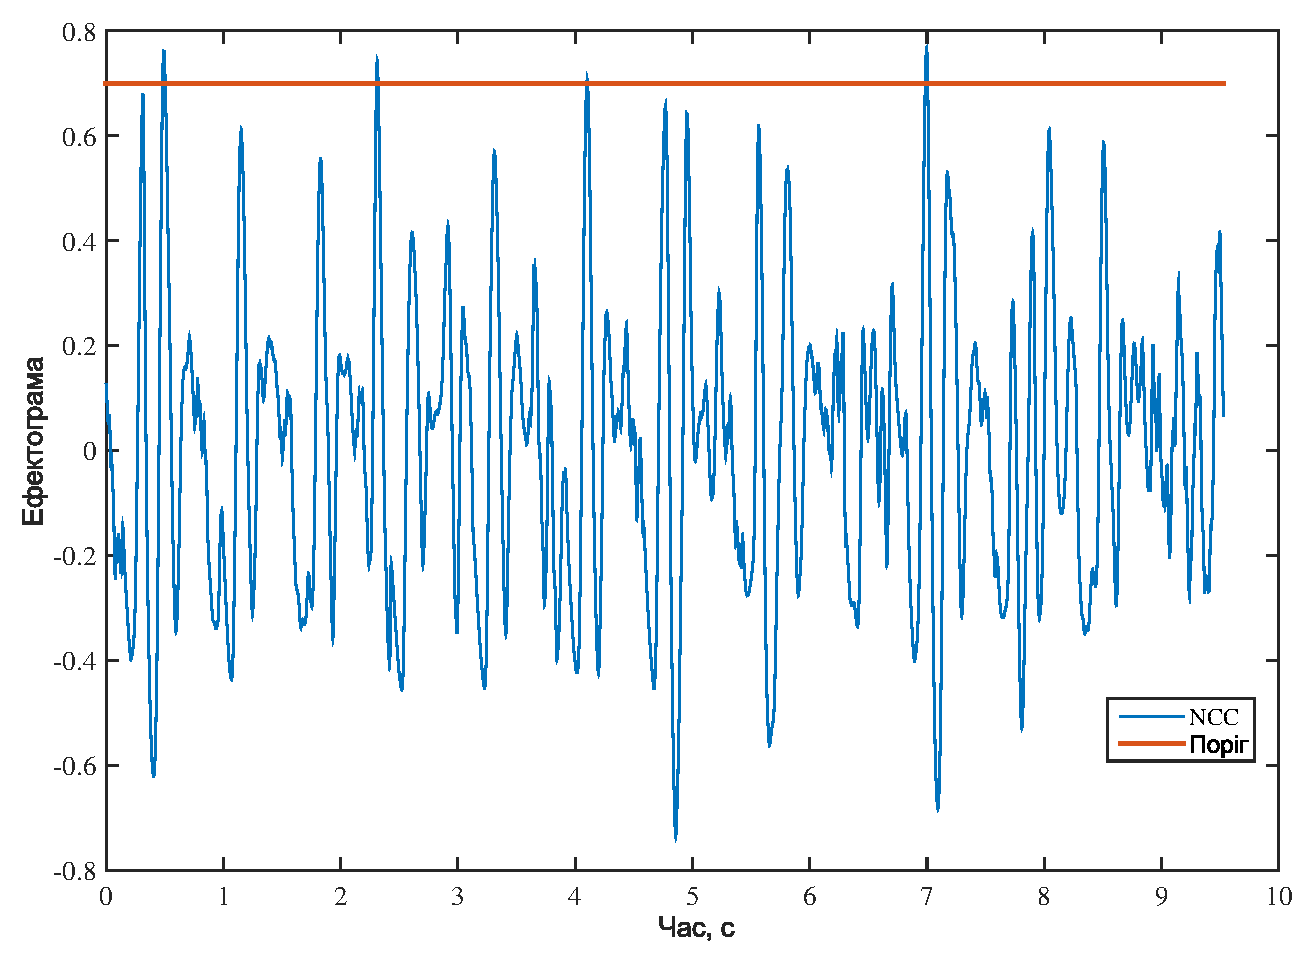
\includegraphics[height=0.28\textheight]{audio-energy-hamming-min-ncc-rect.eps}
            }
            % 2.80

            \subfloat[NSSD]{%
                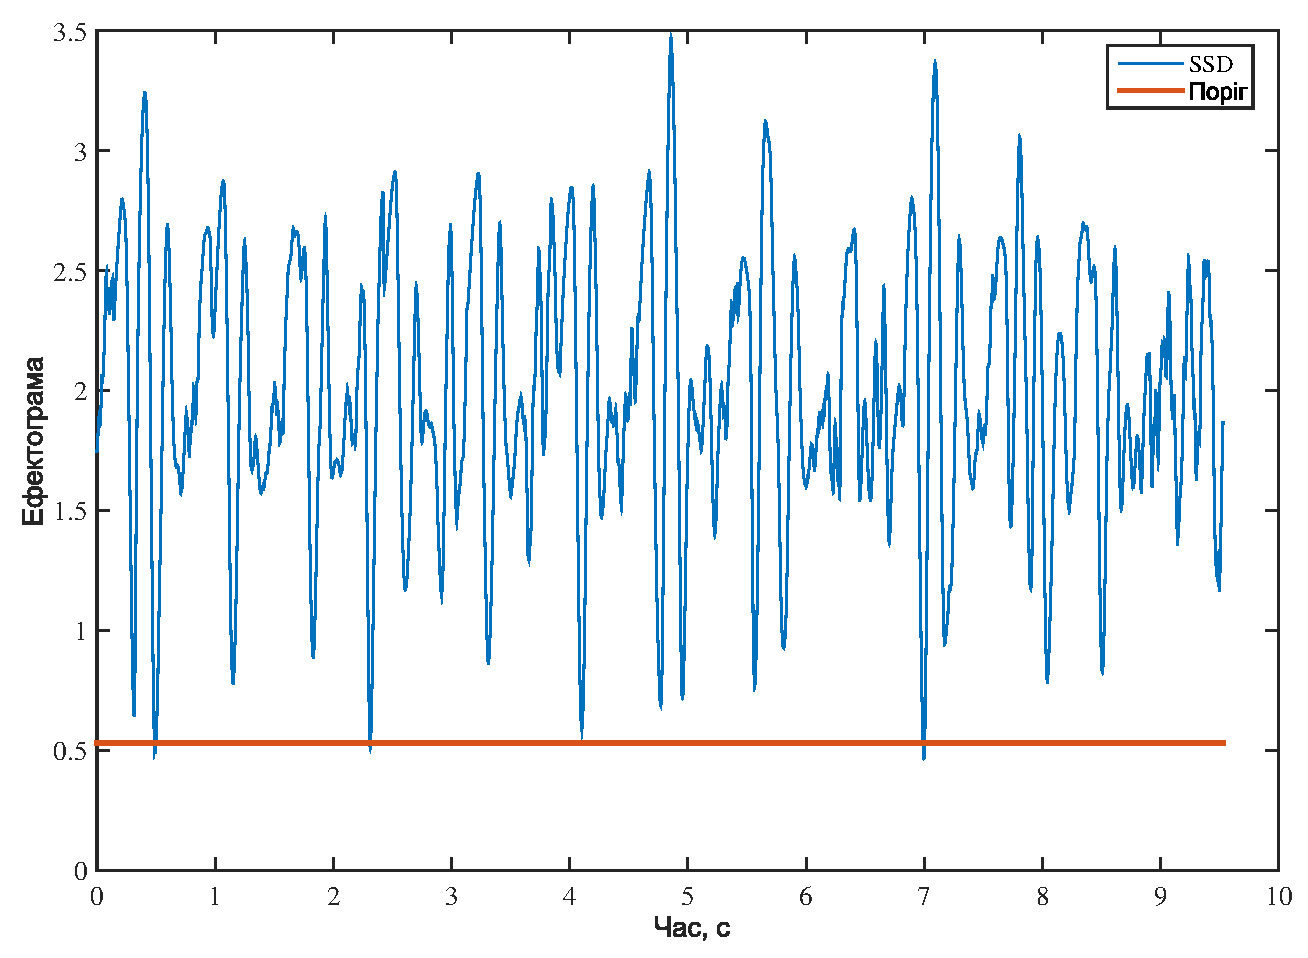
\includegraphics[height=0.28\textheight]{audio-energy-hamming-min-ssd-rect.eps}
            }
            % 2.65

            \subfloat[Kunchenko]{%
                \includegraphics[height=0.28\textheight]{audio-energy-hamming-min-kun-rect.eps}
            }
            % 108.87

            \caption{Знайдений шаблон в енергії, наведеної на рисунку~\ref{fig:audio-energy-hamming-min},
                використовуючи прямокутні вікна}
            \label{fig:matched-energy-hamming-min-rect}
        \end{figure}

        \stepcounter{figurecount}
        \begin{figure}[h]
            \centering
            \subfloat[NCC]{%
                \includegraphics[height=0.28\textheight]{audio-energy-hamming-min-ncc-hamming.eps}
            }
            % 3.26

            \subfloat[NSSD]{%
                \includegraphics[height=0.28\textheight]{audio-energy-hamming-min-ssd-hamming.eps}
            }
            % 3.39

            \subfloat[Kunchenko]{%
                \includegraphics[height=0.28\textheight]{audio-energy-hamming-min-kun-hamming.eps}
            }
            % 130.13

            \caption{Знайдений шаблон в енергії, наведеної на рисунку~\ref{fig:audio-energy-hamming-min},
                використовуючи вікна Геммінга}
            \label{fig:matched-energy-hamming-min-hamming}
        \end{figure}

        \clearpage

\section{Висновки}
    В цьому розділі були успішно проведений статистичний експеримент для дослідження поведінки методів пошуку
    шаблонів, розглянутих в попередніх розділах, як на штучному сигналу, який був згенерований аналітично, так і на
    аудіозаписах мовлення.

    В результаті тестування було виявлено, що:
    \begin{itemize}
        \item Метод поліномів Кунченко дозволяє отримати з точністю, не гіршою за розглянути найпоширеніші методи,
            місцезнаходження шаблону в сигналі, навіть якщо шаблон зазнав змін.
        \item В залежності від типу сигналу, можливо збільшити точність пошуку завдяки використанню віконних функцій у
            методі ковзного вікна.
        \item Завдяки використання коротко"=часової енергії метод поліномів Кунченка дозволяє з високою точністю
            знаходить шаблон в аудіосигналі, що містить у собі запис мовлення.
    \end{itemize}

% vim: spelllang=uk,en spell filetype=tex
